\chapter{剪切自锁问题}
本章讨论另一个自锁问题,中厚板的剪切自锁问题。首先,基于中厚板的本构特性,分析了传统有限元分析过程中产生剪切自锁现象的原因。针对剪切自锁问题,有限元无网格混合离散方案同样适用。随后,根据前文介绍的方法,确定剪切自锁问题的最优约束比,并通过典型弹性力学算例验证其正确性。
\section{中厚板问题}    
考虑如图\ref{ch_5:fig:mindlin_picture}所示中厚板,板厚为$h$,$\Omega$为板中面。在Mindlin假设下,中厚板考虑横向剪切变形,相应的控制方程由下式给出:
\begin{equation}\label{ch_5:eq:strong_mindlin}
    \begin{cases}
        M_{\alpha\beta,\beta} - Q_\alpha = 0 & \textrm{in}\; \Omega \\
        Q_{\alpha,\alpha} + \bar q = 0 & \textrm{in}\; \Omega \\    Q_\alpha n_\alpha = \bar Q & \textrm{on}\; \Gamma_Q \\
        M_{\alpha\beta} n_\beta = \bar M_\alpha & \textrm{on}\; \Gamma_M \\
        \varphi_\alpha = \bar \varphi_\alpha & \textrm{on}\; \Gamma_\varphi \\
        w = \bar w & \textrm{on}\; \Gamma_w \\
    \end{cases}
\end{equation}
\begin{figure}[!h]
    \centering 
        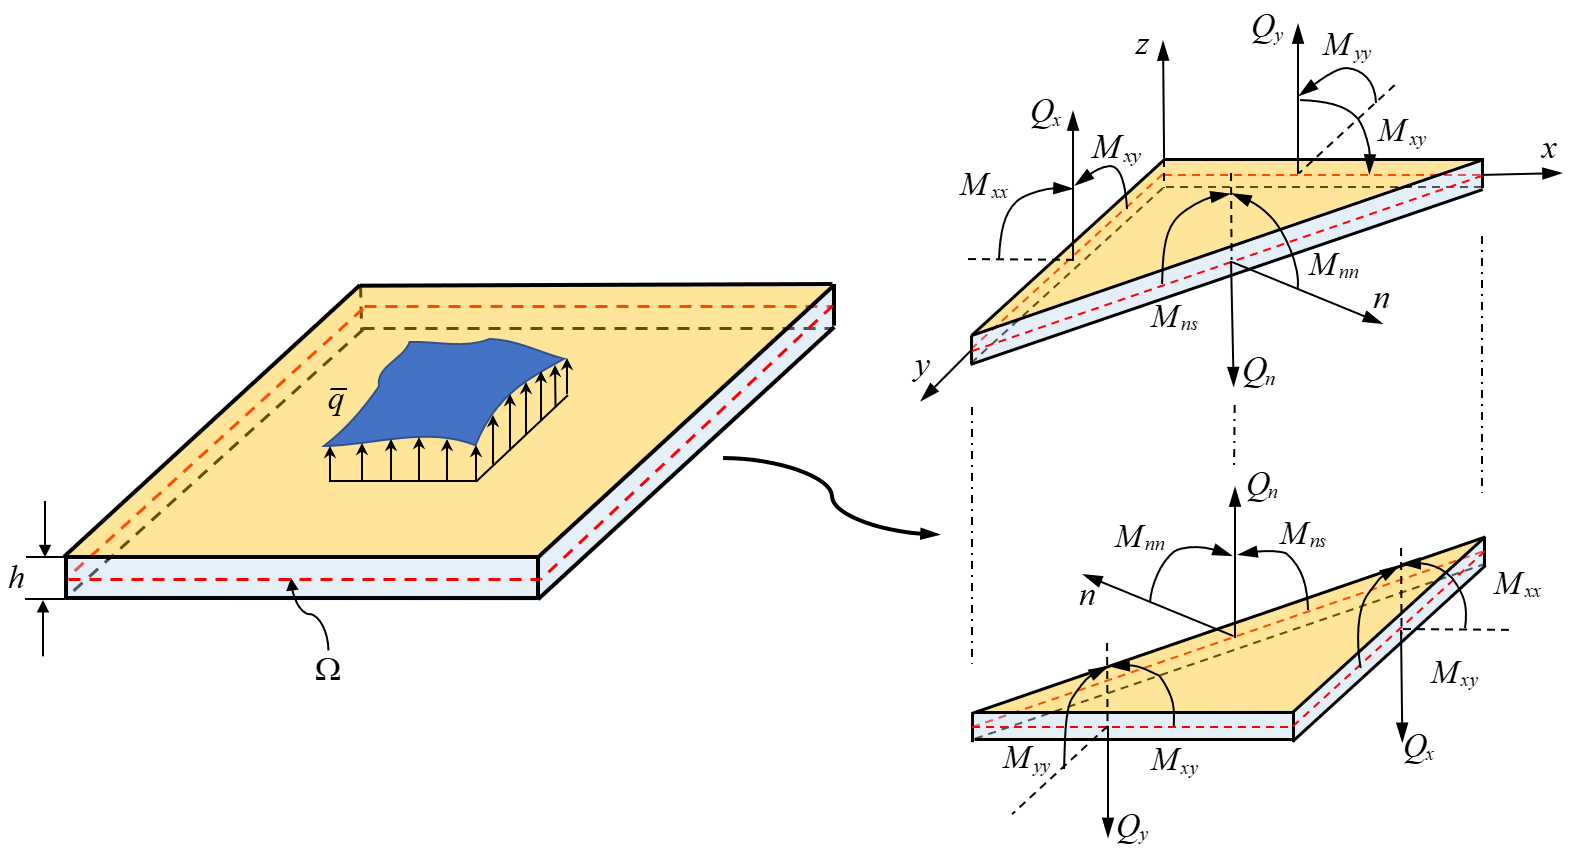
\includegraphics[scale=0.5]{figures/shearlocking/Mindlinplate.png}
        \caption{中厚板运动学及边界条件}\label{ch_5:fig:mindlin_picture}
\end{figure}
式中,$M_{\alpha \beta}$ 可表示弯矩张量$ \boldsymbol{M}$ 的弯曲或扭转部分的分量,$Q_\alpha$为剪力张量$\boldsymbol{Q}$的分量,$\bar{q}$ 为垂直于板中面的分布荷载;
$\Gamma_w$和$\Gamma_\varphi$为本质边界条件,$\bar{w}$和$\bar{\varphi}_\alpha$分别为本质边界条件上给定的挠度和转角;
$\Gamma_Q$ 和$\Gamma_M$ 为自然边界条件,$\bar Q$和$\bar{M}_{\alpha}$ 为自然边界上的等效剪力和法向弯矩;
$n_\alpha$为边界上外法线方向$\pmb{n}$的分量。

在平面应力假设下,对于各同向性线弹性材料,其本构关系表示为:
\begin{equation}\label{ch_5:eq:mindlin_M}
    M_{\alpha \beta}=-\frac{h^3}{12}D_{\alpha \beta \gamma\eta}\kappa_{\gamma\eta}=\frac{h^3}{12}D_{\alpha \beta \gamma\eta}\varphi_{\gamma,\eta}
\end{equation}
\begin{equation}\label{ch_5:eq:mindlin_Q}
    Q_{\alpha}=k\frac{Eh}{2(1+\nu)}\gamma_\beta=kGh(-\varphi_\beta+w_{,\beta})
\end{equation}
其中,$k$为剪切修正系数,$\kappa_{\alpha\beta}$为曲率张量$\pmb\kappa$的分量,$\gamma_\alpha$为剪切应变矢量$\pmb\gamma$的分量,表达式为:
\begin{equation} \label{ch_5:eq:kappa}
    \kappa_{\alpha\beta}=-\varphi_{\alpha,\beta},\quad\gamma_\alpha=-\varphi_\alpha+w_{,\alpha}
\end{equation}
式中$D_{\alpha \beta \gamma\eta}$为在平面应力假设下四阶弹性张量的分量,表达式为:
\begin{equation} 
    D_{\alpha \beta \gamma\eta}=\frac{E}{1-\nu^2}(\nu\delta_{\alpha\beta}\delta_{\gamma\eta}+\frac{1}{2}(1-\nu)(\delta_{\alpha\gamma}\delta_{\beta\eta}+\delta_{\alpha\eta}\delta_{\beta\gamma}))
\end{equation}

根据最小势能原理,强形式\eqref{ch_5:eq:strong_mindlin}所对应的势能泛函表达式为: 
\begin{equation}\label{ch_5:eq:potential_energy}
    \begin{split} 
        \Pi(w,\boldsymbol{\varphi})&=\frac{1}{2}\int_{\Omega}\kappa_{\alpha\beta}M_{\alpha\beta}d\Omega+\frac{1}{2}\int_{\Omega}\gamma_{\alpha}Q_{\alpha}d\Omega\\
        &+\int_{\Gamma_{M}}\varphi_{\alpha}{\bar{M}_{\alpha}}d\Gamma-\int_{\Gamma_{Q}}{w}\bar {Q}d\Gamma-\int_{\Omega} w\bar{q}d\Omega
    \end{split}
\end{equation}
对式\eqref{ch_5:eq:potential_energy}进行变分可得伽辽金弱形式:
\begin{equation}\label{ch_5:eq:weak_penalty_mindlin}
    \begin{split} 
        \text{Find}\,&(w,\varphi_{\alpha})\in V\\
        &\int_{\Omega}\delta\kappa_{\alpha\beta}M_{\alpha\beta}d\Omega+\int_{\Omega}\delta\gamma_{\alpha}Q_{\alpha}d\Omega=\\
        &-\int_{\Gamma_{M}}\delta\varphi_{\alpha}{\bar{M}_{\alpha}}d\Gamma+\int_{\Gamma_{Q}}{\delta{w}}\bar {Q}d\Gamma+\int_{\Omega} \delta{w}\bar{q}d\Omega,\quad \forall(\delta w,\delta\varphi_{\alpha}) \in V
    \end{split}
\end{equation}

对于考虑横向剪切变形的中厚板,根据中厚板的本构关系\eqref{ch_5:eq:mindlin_M},\eqref{ch_5:eq:mindlin_Q},当其厚度减小$h\rightarrow 0$,$h \gg h^3$将导致弯矩$M_{\alpha \beta}$减小的速度远大于剪力$Q_{\alpha}$,使得$Q_{\alpha}\gg M_{\alpha \beta}$。从式\eqref{ch_5:eq:weak_penalty_mindlin}中可以看出当$Q_{\alpha}\gg M_{\alpha \beta}$,剪切应变$\boldsymbol{\gamma}$被约束,导致板的剪切位移为$0$。

在传统有限元法中,整个板中面$\Omega$由一组具有节点$\{\boldsymbol x_I\}_{I=1}^{n_u}$的构造网格离散,其中$n_u$是节点的数量。
挠度$w$及其变分$\delta w $,转角$\varphi_\alpha$及其变分$\delta \varphi_\alpha $可通过$x_I$处的节点系数和形函数进行近似:
\begin{equation}\label{ch_5:eq:w_h}
    w^h(\boldsymbol x) = \sum_{I=1}^{n_u} N_I(\boldsymbol x) w_I, \quad \delta w^h(\boldsymbol x) = \sum_{I=1}^{n_u} N_I(\boldsymbol x) \delta w_I
\end{equation}
\begin{equation}\label{ch_5:eq:varphi_h}
    \varphi^h_{\alpha}(\boldsymbol x) = \sum_{I=1}^{n_u} N_I(\boldsymbol x) \varphi_{\alpha I}, \quad \delta \varphi^h_{\alpha}(\boldsymbol x) = \sum_{I=1}^{n_u} N_I(\boldsymbol x) \delta \varphi_{\alpha I}
\end{equation}
其中,$N_I$为节点$x_I$处的形函数,$w_I$和$\varphi_{\alpha I}$节点系数张量。

结合式\eqref{ch_5:eq:kappa},\eqref{ch_5:eq:w_h}和\eqref{ch_5:eq:varphi_h},相应的近似曲率$\boldsymbol\kappa^h$和近似剪切应变$\boldsymbol\gamma^h$及其变分可表示为:
\begin{equation}
    \boldsymbol\kappa^h = 
    \begin{Bmatrix}
        \kappa^h_{11} \\ \kappa^h_{22} \\ 2\kappa^h_{12} 
    \end{Bmatrix} = -\sum_{I=1}^{n_u}
    \begin{bmatrix}
        0 & N_{I,1} & 0 \\ 0 & 0 & N_{I,2} \\ 0 & N_{I,2} & N_{I,1}
    \end{bmatrix}
    \begin{Bmatrix}
        w_I \\ \varphi_{1I} \\ \varphi_{2I}
    \end{Bmatrix} = - \sum_{I=1}^{n_u} \boldsymbol B^b_I \boldsymbol d_I
\end{equation}
\begin{equation}
    \boldsymbol\gamma^h = 
    \begin{Bmatrix}
        \gamma^h_1 \\ \gamma^h_2
    \end{Bmatrix} = \sum_{I=1}^{n_u}
    \begin{bmatrix}
        N_{I,1} & N_I & 0 \\
        N_{I,2} & 0 & N_I
    \end{bmatrix}
    \begin{Bmatrix}
        w_I \\ \varphi_{1I} \\ \varphi_{2I}
    \end{Bmatrix} = \sum_{I=1}^{n_u} \boldsymbol B^s_I \boldsymbol d_I
\end{equation}
\begin{equation}\label{ch_5:eq:kappa_h}
    \delta\boldsymbol\kappa^h = - \sum_{I=1}^{n_u} \boldsymbol B^b_I \delta\boldsymbol d_I ,\quad \delta\boldsymbol\gamma^h = \sum_{I=1}^{n_u} \boldsymbol B^s_I \delta\boldsymbol d_I
\end{equation}

将式\eqref{ch_5:eq:kappa_h}代入到弱形式\eqref{ch_5:eq:weak_penalty_mindlin}可得下列里兹--伽辽金问题:
\begin{equation}\label{ch_5:eq:ritz_penalty_mindlin}
    \begin{split} 
        \text{Find}\,&(w^h,\boldsymbol{\varphi}^h_{\alpha})\in V_h\\
        &\int_{\Omega}\delta\kappa^h_{\alpha\beta}M_{\alpha\beta}d\Omega+\int_{\Omega}\delta\gamma^h_{\alpha}Q_{\alpha}d\Omega=\\
        &-\int_{\Gamma_{M}}\delta\varphi^h_{\alpha}{\bar{M}_{\alpha}}d\Gamma+\int_{\Gamma_{Q}}{\delta{w^h}}\bar {Q}d\Gamma+\int_{\Omega} \delta{w^h}\bar{q}d\Omega,\quad \forall(\delta w^h,\delta\varphi^h_{\alpha}) \in V_h
    \end{split}
\end{equation}
根据$\delta\boldsymbol\kappa^h$和$\delta\boldsymbol\gamma^h$的任意性,上述方程可简化为如下离散控制方程:
\begin{equation}\label{ch_5:eq:equilibrium_penalty}
    (\boldsymbol K^b + \boldsymbol K^s) \boldsymbol d = \boldsymbol f
\end{equation}
其中,$\boldsymbol K^b$为弯曲刚度矩阵,$\boldsymbol K^s$为剪切刚度矩阵,$\pmb{f}$为力向量,其分量具有以下形式:
\begin{equation}\label{ch_5:eq:stiffness_bending}
    \boldsymbol K^b_{IJ} = \frac{h^3}{12} \int_\Omega \boldsymbol B^{bT}_I \boldsymbol D \boldsymbol B^b_J d\Omega\\
\end{equation}
\begin{equation}\label{ch_5:eq:stiffness_shear}
    \boldsymbol K^s_{IJ} = h \int_\Omega \boldsymbol B^{sT}_I kG \boldsymbol B^s_J d\Omega
\end{equation}
\begin{equation}
    \boldsymbol f_I = \int_{\Gamma_Q} N_I \bar{\boldsymbol Q} d\Gamma - \int_{\Gamma_M} N_I \bar{\boldsymbol M} d\Gamma + \int_\Omega N_I \bar{\boldsymbol q} d\Omega
\end{equation}
式中,$\boldsymbol{D}$为平面应力弹性矩阵,等效剪力$\bar{\boldsymbol Q}$,法向弯矩$\bar{\boldsymbol M}$,分布荷载$\bar{\boldsymbol q}$的分量分别为:
\begin{equation}
    \bar{\boldsymbol Q} =  
    \begin{Bmatrix}
        \bar Q \\ 0 \\ 0
    \end{Bmatrix},
        \bar{\boldsymbol M} =
    \begin{Bmatrix}
        0 \\ \bar M_1 \\ \bar M_2
    \end{Bmatrix},
        \bar{\boldsymbol q} =
    \begin{Bmatrix}
        \bar q \\ 0 \\ 0
    \end{Bmatrix}
\end{equation}

\section{中厚板问题有限元无网格混合离散方案} 
同样,由式\eqref{ch_5:eq:equilibrium_penalty},\eqref{ch_5:eq:stiffness_bending}和\eqref{ch_5:eq:stiffness_shear}可知,对于中厚板,当外力向量具有一定的数值时,厚度$h$减小$h\rightarrow 0$将导致剪切刚度矩阵$\boldsymbol{K^s}$中的所有模态也趋向零。此时,剪切刚度矩阵$\boldsymbol{K^s}$可作为罚函数项将剪切刚度中所有模态约束住,厚度$h$为其中的罚因子。用传统有限元法进行求解时,由于离散的有限元近似阶次较低,导致过多的位移自由度受到剪切约束的限制,位移解将远小于实际情况,即出现剪切自锁现象。  

前文提到的缓解体积自锁问题的方法同样适用于缓解剪切自锁问题。对于剪切自锁问题,同样可以采用有限元无网格混合离散方案,引入剪切应力$\boldsymbol{Q}$作为拉格朗日乘子独立变量,可以得到拉格朗日乘子型剪切约束施加方案。此时能量泛函具有挠度$w$、转角$\boldsymbol{\varphi}$和剪切应力$\boldsymbol{Q}$三个变量,势能泛函的表达式可更改为:
\begin{equation}\label{ch_5:eq:potential_energy_mixed}
    \begin{split} 
        \Pi(w,\boldsymbol{\varphi},\boldsymbol{Q})&=\int_{\bar\Omega}\frac{1}{2}\varepsilon_{ij}\sigma_{ij} d\Omega+\frac{1}{2}\int_{\Omega}Q_{\alpha}(\gamma_{\alpha}-\frac{Q_{\alpha}}{kGh})d\Omega-\int_{\Gamma^{t}} u_{i}t_{i}d\Gamma-\int_{\Omega} u_{i}b_{i}d\Omega\\
        &=\frac{1}{2}\int_{\Omega}(\kappa_{\alpha \beta}M_{\alpha \beta}+\gamma_{\alpha}Q_{\alpha})d\Omega+\frac{1}{2}\int_{\Omega}Q_{\alpha}(\gamma_{\alpha}-\frac{Q_{\alpha}}{kGh})d\Omega\\
        &+\int_{\Gamma_{M}}\varphi_{\alpha}{\bar{M}_{\alpha}}d\Gamma-\int_{\Gamma_{Q}}{w}\bar {Q}d\Gamma-\int_{\Omega} w\bar{q}d\Omega
    \end{split}
\end{equation}

对式\eqref{ch_5:eq:potential_energy_mixed}进行变分可得伽辽金弱形式:
\begin{equation} 
    \begin{split}
    &\delta\Pi(w,\boldsymbol\varphi,\boldsymbol{Q})\\
    &=\int_{\Omega}\delta\kappa_{\alpha \beta}M_{\alpha \beta}d\Omega+\frac{1}{2}\int_{\Omega}\delta\gamma_{\alpha}Q_{\alpha}d\Omega+\frac{1}{2}\int_{\Omega}\gamma_{\alpha}\delta{Q}_{\alpha}d\Omega+\frac{1}{2}\int_{\Omega}\delta\gamma_{\alpha}Q_{\alpha}d\Omega\\
    &+\frac{1}{2}\int_{\Omega}\gamma_{\alpha}\delta{Q}_{\alpha}d\Omega-\int_{\Omega}\frac{\delta{Q}_{\alpha}{Q}_{\alpha}}{kGh}d\Omega+\int_{\Gamma_{M}}\delta\varphi_{\alpha}{{\bar M}_{\alpha}}d\Gamma-\int_{\Gamma_{Q}}\delta{w}{\bar Q}d\Gamma+\int_{\Omega} \delta{w}\bar{q}d\Omega\\
    &=\int_{\Omega}\delta\kappa_{\alpha \beta}M_{\alpha \beta}d\Omega+\int_{\Omega}\delta\gamma_{\alpha}Q_{\alpha}d\Omega+\int_{\Omega}\gamma_{\alpha}\delta{Q}_{\alpha}d\Omega-\int_{\Omega}\frac{\delta{Q}_{\alpha}{Q}_{\alpha}}{kGh}d\Omega+\int_{\Gamma_{M}}\delta\varphi_{\alpha}{\boldsymbol{\bar M}_{\boldsymbol{\alpha}}}d\Gamma\\
    &-\int_{\Gamma_{Q}}\delta{w}{\bar Q}d\Gamma+\int_{\Omega} \delta{w}\bar{q}d\Omega=0
    \end{split}
\end{equation}
上述伽辽金弱形式可以改写为:
\begin{flalign}
    &\text{Find}\, \boldsymbol u=(w,\boldsymbol{\varphi}) \in V, \boldsymbol p \in Q&\nonumber
\end{flalign}
\begin{equation}\label{ch_5:eq:weak_mix}
    \begin{aligned}
        a(\delta \boldsymbol u, \boldsymbol u) + b(\delta \boldsymbol u,\boldsymbol p) &= f(\delta \boldsymbol u) \quad &\forall \delta \boldsymbol u \in V \\
        b(\boldsymbol u, \delta \boldsymbol p) +  c(\delta \boldsymbol p,\boldsymbol p)&= \boldsymbol 0 \quad &\forall \delta \boldsymbol p \in Q
    \end{aligned}
\end{equation}
具体表达式为:
\begin{equation}\label{ch_5:eq:mindlin_weak1}
    \int_{\Omega}\delta\kappa_{\alpha \beta}M_{\alpha \beta}d\Omega+\int_{\Omega}\delta\gamma_{\alpha}Q_{\alpha}d\Omega=\int_{\Gamma_{Q}}\delta{w}{\bar Q}d\Gamma-\int_{\Omega} \delta{w}\bar{q}d\Omega-\int_{\Gamma_{M}}\delta\varphi_{\alpha}{{\bar M}_{\alpha}}d\Gamma
\end{equation}
\begin{equation}\label{ch_5:eq:mindlin_weak2}
    \int_{\Omega}\gamma_{\alpha}\delta{Q}_{\alpha}d\Omega-\int_{\Omega}\frac{\delta{Q}_{\alpha}{Q}_{\alpha}}{kGh}d\Omega=0
\end{equation}

采用伽辽金法进行求解时,挠度$w$、转角$\boldsymbol{\varphi}$和剪切应力$\boldsymbol{Q}$可以采用不同的离散方式进行近似,形成混合离散框架。挠度$w$和转角$\boldsymbol{\varphi}$采用有限元形函数\eqref{ch_5:eq:w_h},\eqref{ch_5:eq:varphi_h}进行近似,剪切应力$\boldsymbol{Q}$通过再生核无网格形函数\eqref{ch_4:eq:mfshapefunction}进行近似,近似的剪切应力$\boldsymbol{Q}^h$及其变分可表示为:
\begin{equation}\label{ch_5:eq:Q_h}
    Q^h_\alpha(\boldsymbol x) = \sum_{K=1}^{n_q} \psi_K(\boldsymbol x) \boldsymbol{q}_{K},\quad \delta Q^h_\alpha(\boldsymbol x) = \sum_{K=1}^{n_q} \psi_K(\boldsymbol x) \delta \boldsymbol{q}_{ K}
\end{equation}
其中,$\boldsymbol{q}_{ K}$是节点系数,$\psi_K$是对应的形函数。

根据$\delta\boldsymbol\kappa^h$、$\delta\boldsymbol\gamma^h$和$\delta\boldsymbol Q^h$的任意性,式\eqref{ch_5:eq:weak_mix}可简化为如下离散控制方程:
\begin{equation} \label{equilibrium_mindlin_mix}
    \begin{bmatrix}\boldsymbol{K}^{b}&\boldsymbol{K}^{sq}\\{\boldsymbol{K}^{sq}}^T&\boldsymbol{K}^{qq}\end{bmatrix}
    \begin{Bmatrix}\boldsymbol{d}\\\boldsymbol{q}\end{Bmatrix}=
    \begin{Bmatrix}\boldsymbol{f}\\\boldsymbol{0}\end{Bmatrix}
\end{equation}
式中,$\boldsymbol K^{sq}$为刚度矩阵中和位移、剪切应力都有关的部分,$\boldsymbol K^{qq}$为刚度矩阵中只和剪切应力相关的部分,其分量分别为:
\begin{equation} 
    \boldsymbol K^{sq}_{IK} = \int_\Omega \boldsymbol B^{sT}_I \psi_K d\Omega
\end{equation} 
\begin{equation} 
    \boldsymbol K^{qq}_{KL} = -\frac{1}{kGh} \int_\Omega \psi_K \psi_L \boldsymbol 1 d\Omega
\end{equation}


\section{数值算例}
\subsection{固支方板问题}
如图\ref{ch_5:fig:plate}所示,一固支方板求解域为$\Omega=(0,1)\otimes(0,1)$,边长$L=1$,厚度为$h$,材料系数分别为杨氏模量$E=10.92\times10^6$、泊松比$\nu=0.3$板面内分布如图所示纵向非均布荷载:
\begin{equation} 
\begin{split} 
    \bar{q}(x,y) =&\frac{Eh^3}{12(1-\nu^2)}(12y(y-1)(5x^2-5x+1)(2y^2(y-1)^2+x(x-1)(5y^2-5y+\\
    &1))+12x(x-1)(5y^2-5y+1)(2x^2(x-1)^2+y(y-1)(5x^2-5x+1)))
\end{split} 
\end{equation}
该问题的精确解为:
\begin{equation} 
    \begin{split} 
        w(x,y) =&\frac{1}{3}x^3(x-1)^3y^3(y-1)^3-\frac{2h^2}{5(1-\nu)}(y^3(y-1)^3x(x-1)(5x^2-5x+1)+\\
        &x^3(x-1)^3y(y-1)(5y^2-5y+1))\\
        \theta_1(x,y) =& y^3(y-1)^3x^2(x-1)^2(2x-1)\\
        \theta_2(x,y) =& x^3(x-1)^3y^2(y-1)^2(2y-1)
    \end{split} 
\end{equation}
\begin{figure}[!h]
    \centering 
        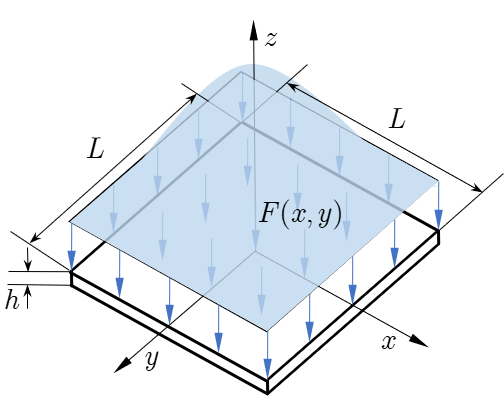
\includegraphics[scale=0.8]{figures/shearlocking/plate.png}
        \caption{固支方板问题模型}\label{ch_5:fig:plate}
\end{figure}

为研究误差收敛性,采用图\ref{ch_5:fig:platemsh}所示的均布的81、289、1089、4225
的四个疏密不同的节点进行离散,并采用线性单元:三角形三节点单元(Tri3)、四边形四节点单元(Quad4),二次单元:
三角形六节点单元(Tri6)、四边形八节点单元(Quad8)。此时对于采用对于线性基函数的固支方板问题其影响域取为1.5倍
的积分域长度,采用二次基函数时其影响域取为2.5倍积分域长度。

如图\ref{ch_5:fig:linear-l2}为固支方板问题线性单元位移误差对比图。从图中可以看出线性单元传统有限元方法在厚度为$0.1$时能达到理论误差收敛率但计算精度低于混合离散法,在厚度为$0.01$,$0.001$时无法到达理论误差收敛率,产生了剪切自锁现象。混合离散法在三个厚度均能达到理论误差收敛率。图\ref{ch_5:eq:quad-l2}为固支方板问题二次单元位移误差对比图。从图中可以看出二次单元传统有限元方法在厚度为$0.1$时能达到理论误差收敛率且计算精度与混合离散方法相当,在厚度为$0.01$时能达到理论误差收敛率但计算精度低于混合离散方法,在厚度为$0.001$时无法到达理论误差收敛率。
\begin{figure}[!h]
    \centering 
    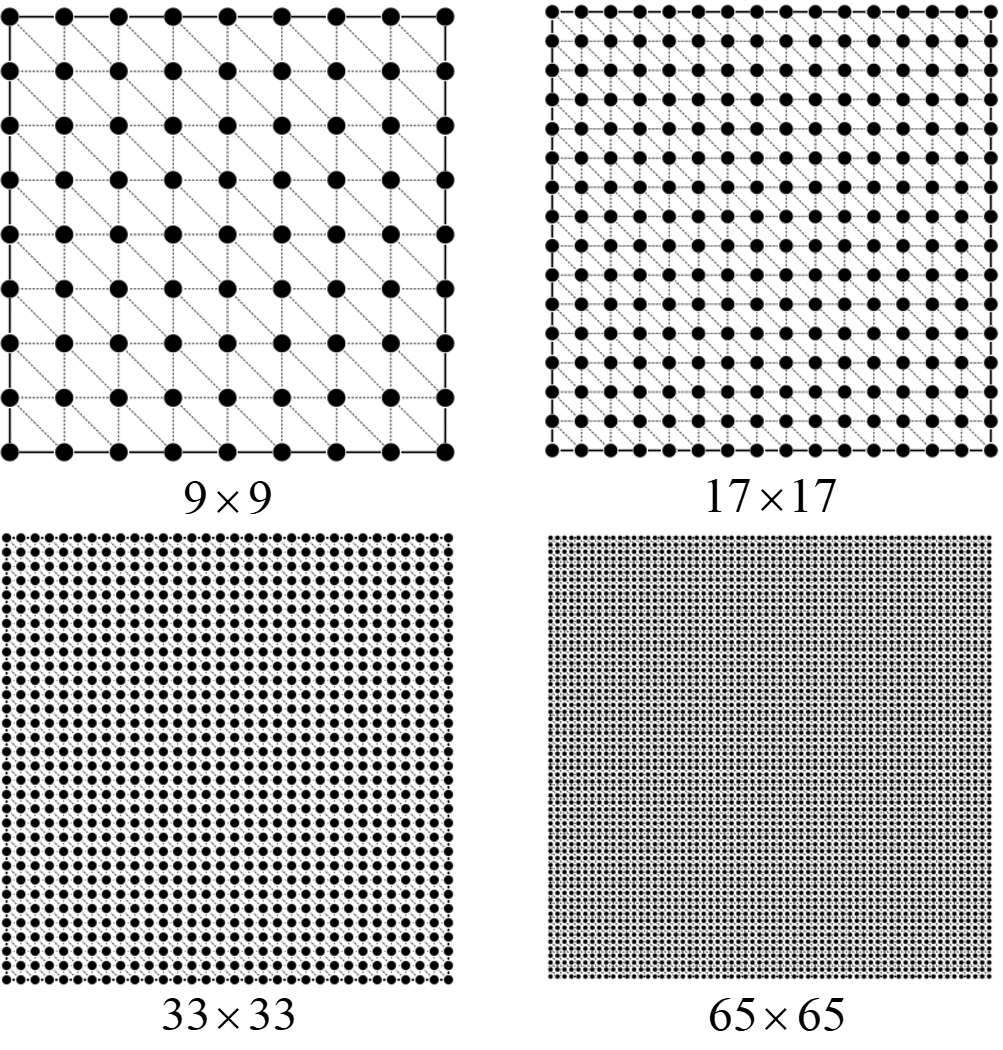
\includegraphics[scale=0.5]{figures/shearlocking/platemsh.png}
    \caption{固支方板问题节点离散}\label{ch_5:fig:platemsh}
\end{figure}
\begin{figure}[!h]
    \centering
    \begin{subcaptiongroup}
    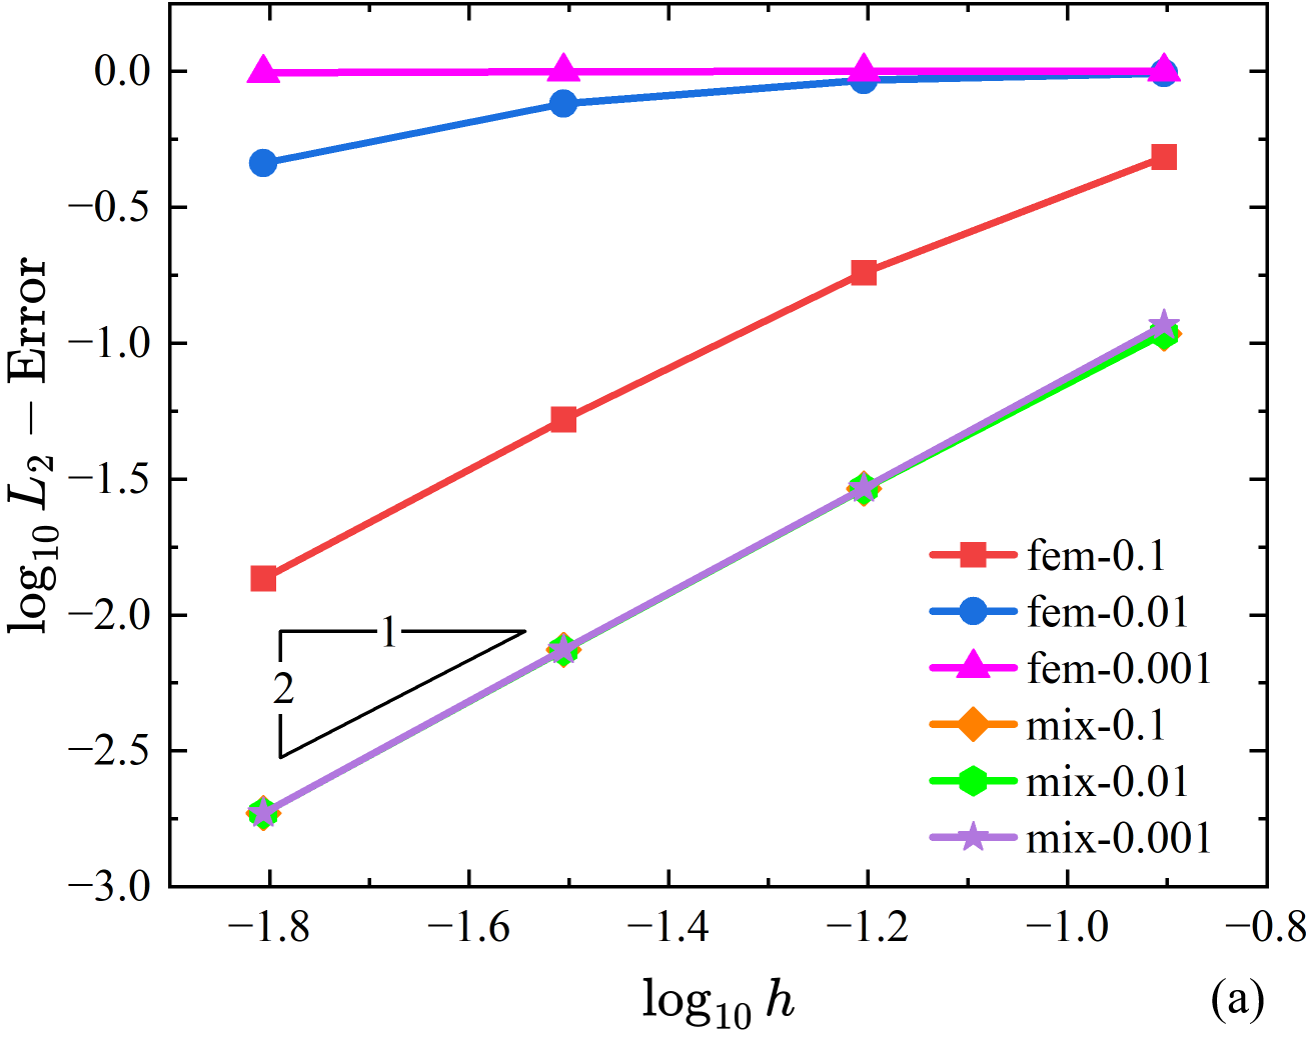
\includegraphics[width=0.49\textwidth]{figures/shearlocking/T3-l2-h.png}
    \phantomcaption\label{T3-l2-h}
    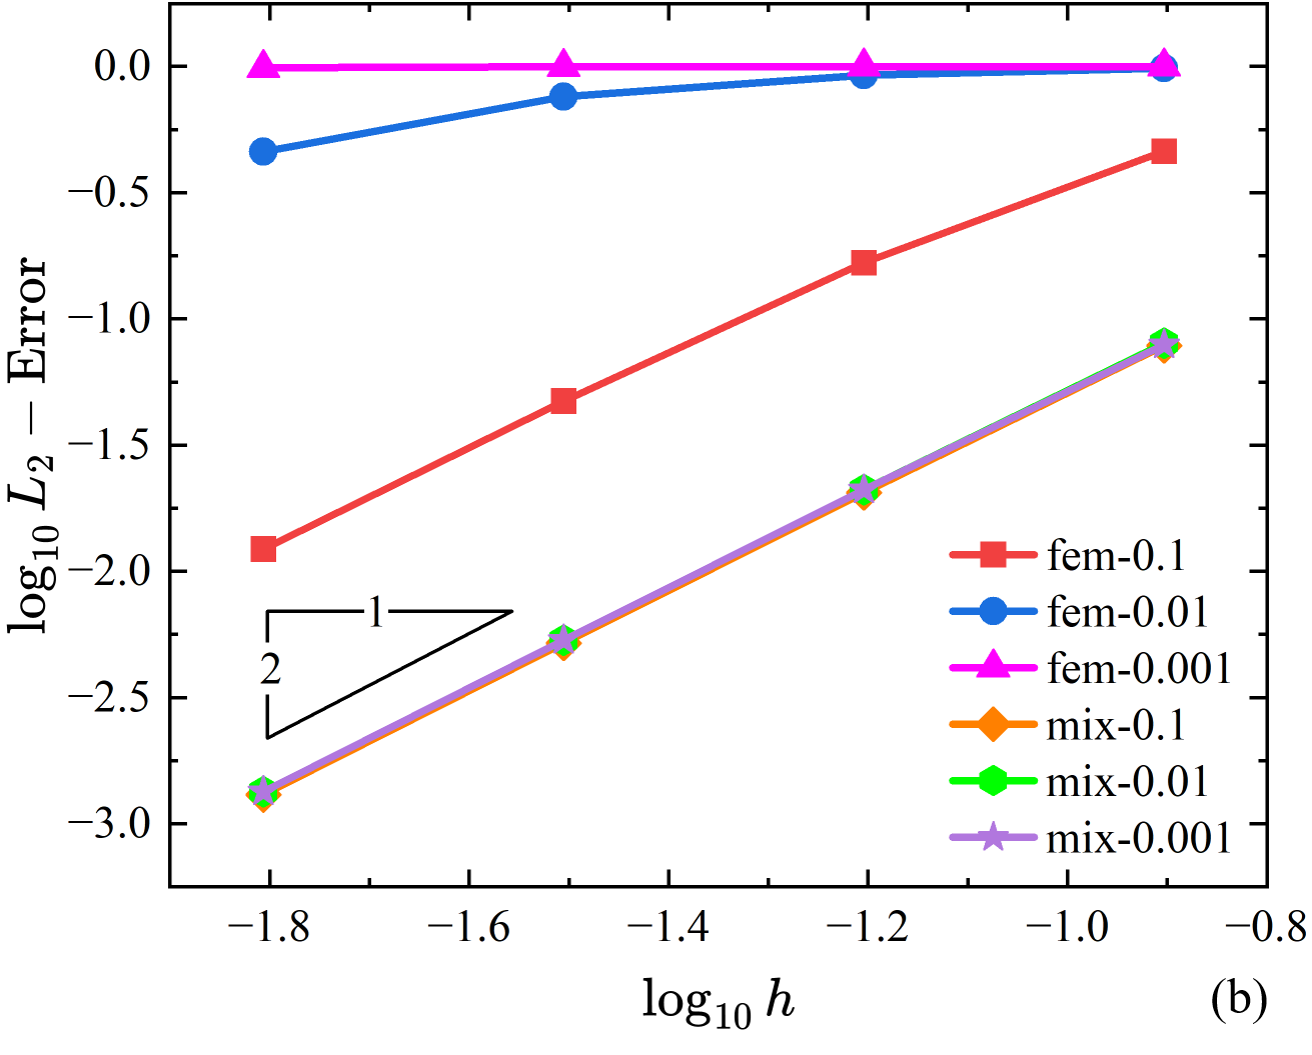
\includegraphics[width=0.49\textwidth]{figures/shearlocking/Q4-l2-h.png}
    \phantomcaption\label{Q4-l2-h}
    \end{subcaptiongroup}
\caption{\centering{固支方板问题线性单元误差对比:\protect\linebreak \subref{T3-l2-h} Tri3单元$L_2$误差;\subref{Q4-l2-h}Quad4单元 $L_2$误差}}
\label{ch_5:fig:linear-l2}
\end{figure}
\begin{figure}[!h]
    \centering
    \begin{subcaptiongroup}
    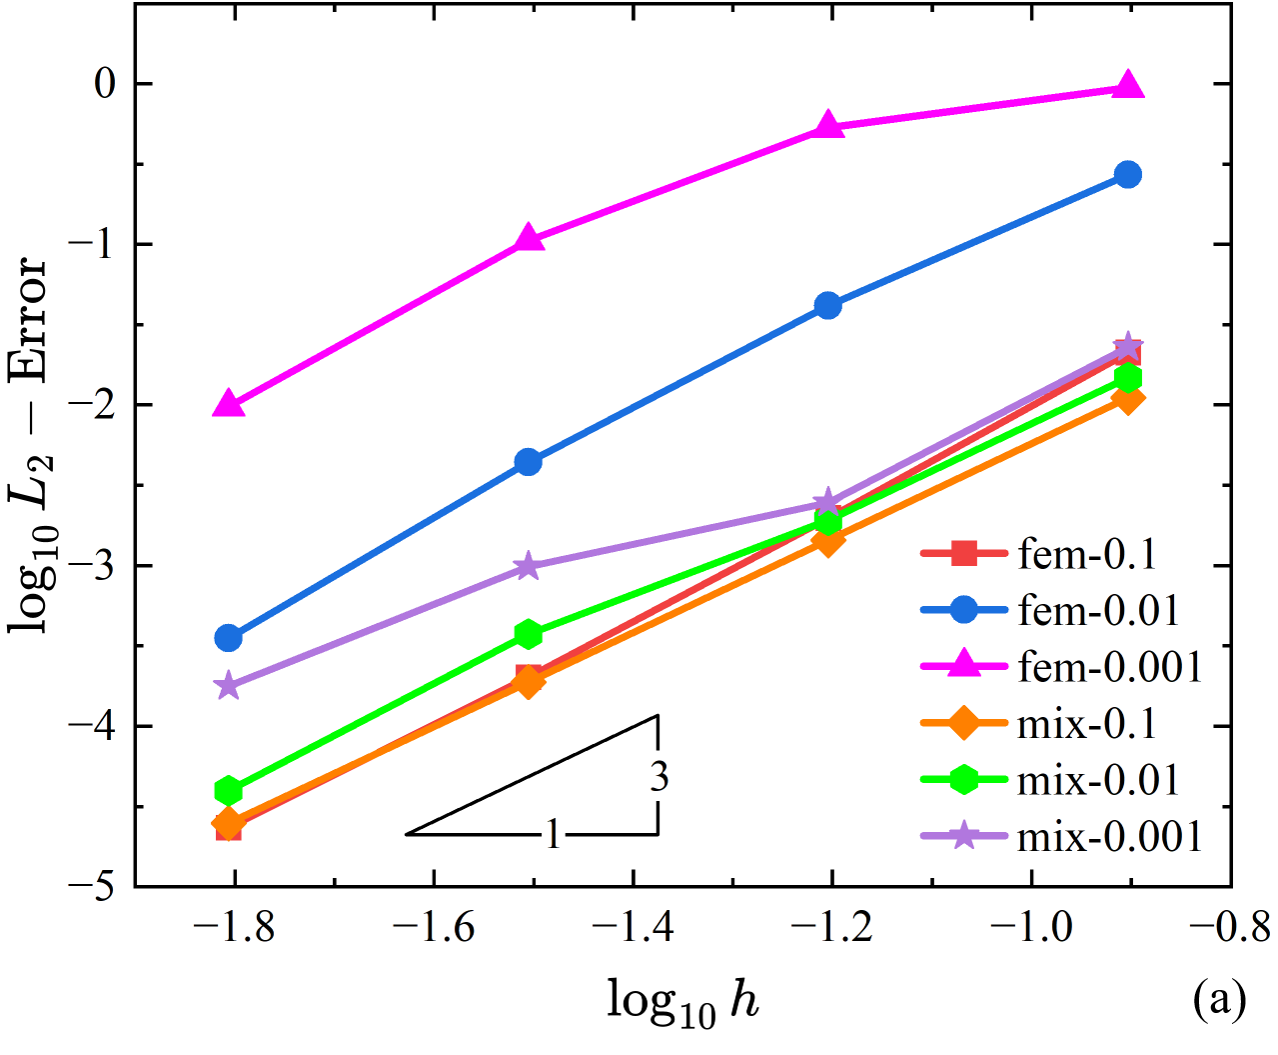
\includegraphics[width=0.49\textwidth]{figures/shearlocking/T6-l2-h.png}
    \phantomcaption\label{T6-l2-h}
    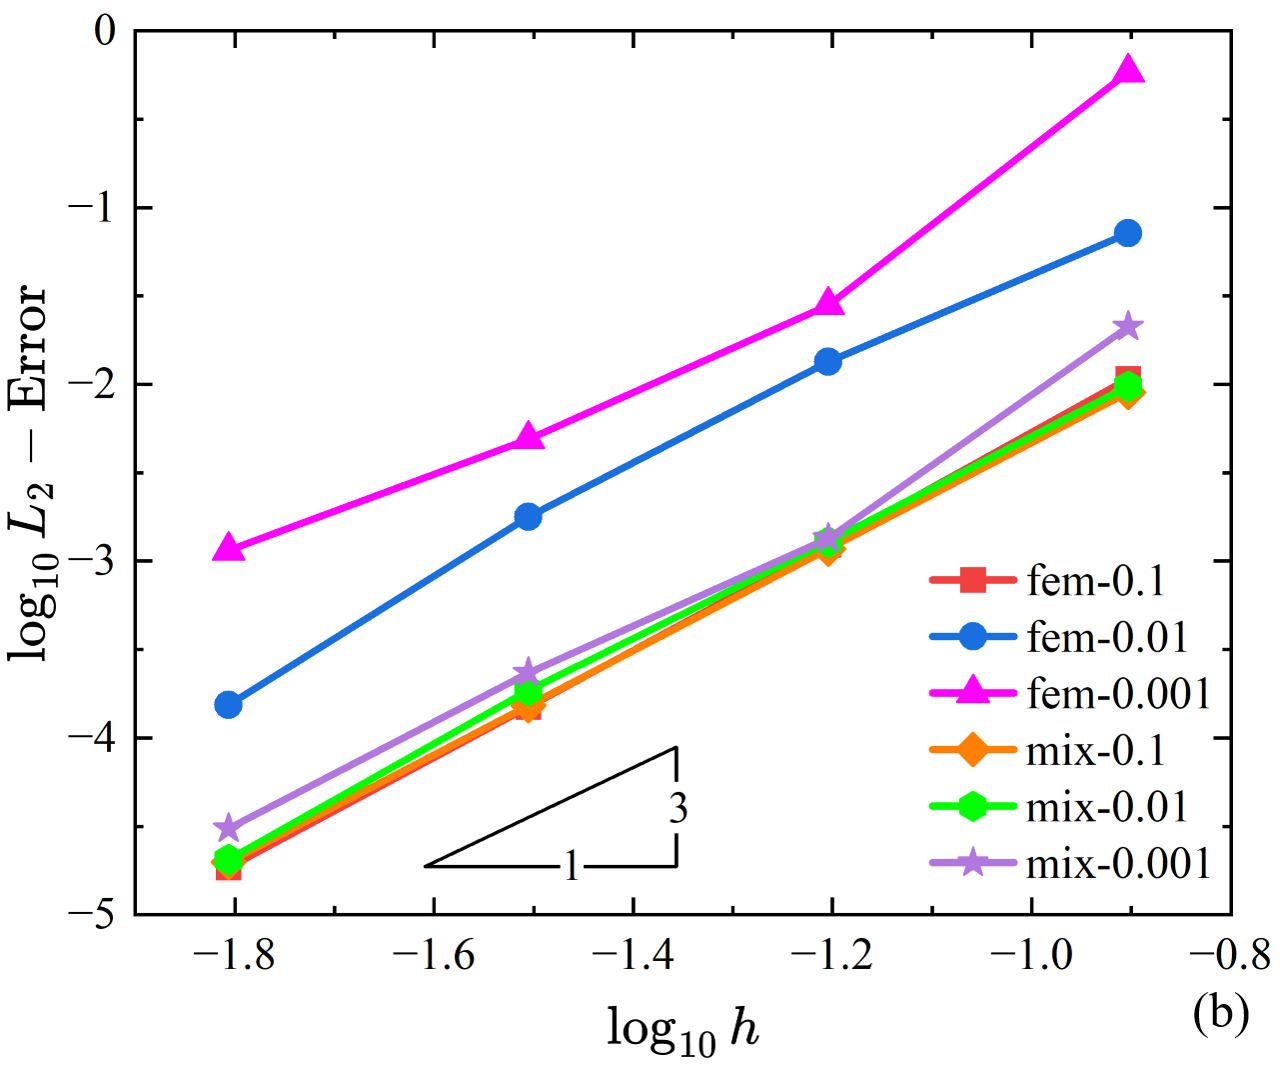
\includegraphics[width=0.49\textwidth]{figures/shearlocking/Q8-l2-h.png}
    \phantomcaption\label{Q8-l2-h}
    \end{subcaptiongroup}
\caption{\centering{固支方板问题二次单元误差对比:\protect\linebreak \subref{T6-l2-h} Tri6单元$L_2$误差;\subref{Q8-l2-h}Quad8单元 $L_2$误差}}
\label{ch_5:eq:quad-l2}
\end{figure}

位移分别采用图\ref{ch_5:fig:platemsh}所示的网格单元,通过改变剪切应力节点的数量,验证剪切应力节点数量与误差的关系。图\ref{ch_5:fig:linear_ns}、\ref{ch_5:fig:quad_ns}为相对应的结果。
图\ref{ch_5:fig:linear_ns}为线性单元剪切应力节点数量与误差的关系,其中Tri3单元和Quad4单元的位移节点数量一致。
图(a),(b)最优应力节点数为,分析结果显示,随着应力节点数量的减少位移误差率先达到最小值,而应力误差虽有所下降但其值始终保持在较高水平。
图(c),(d)和图(e)(f)的最优应力节点数分别为。分析结果显示,应力节点数量的减少位移误差同样先达到最小值。
值得注意的是,在约束比达到最优值附近时,应力误差也会随之达到最小值。
图\ref{ch_5:fig:quad_ns}为二次单元剪切应力节点数量与误差的关系,图(a),(b)最优应力节点数分别为,对于二次单元同样具有上述效果。这一现象在所有节点数量条件下均得到了验证。

\begin{figure}[!h]
    \centering
    \begin{subcaptiongroup}
    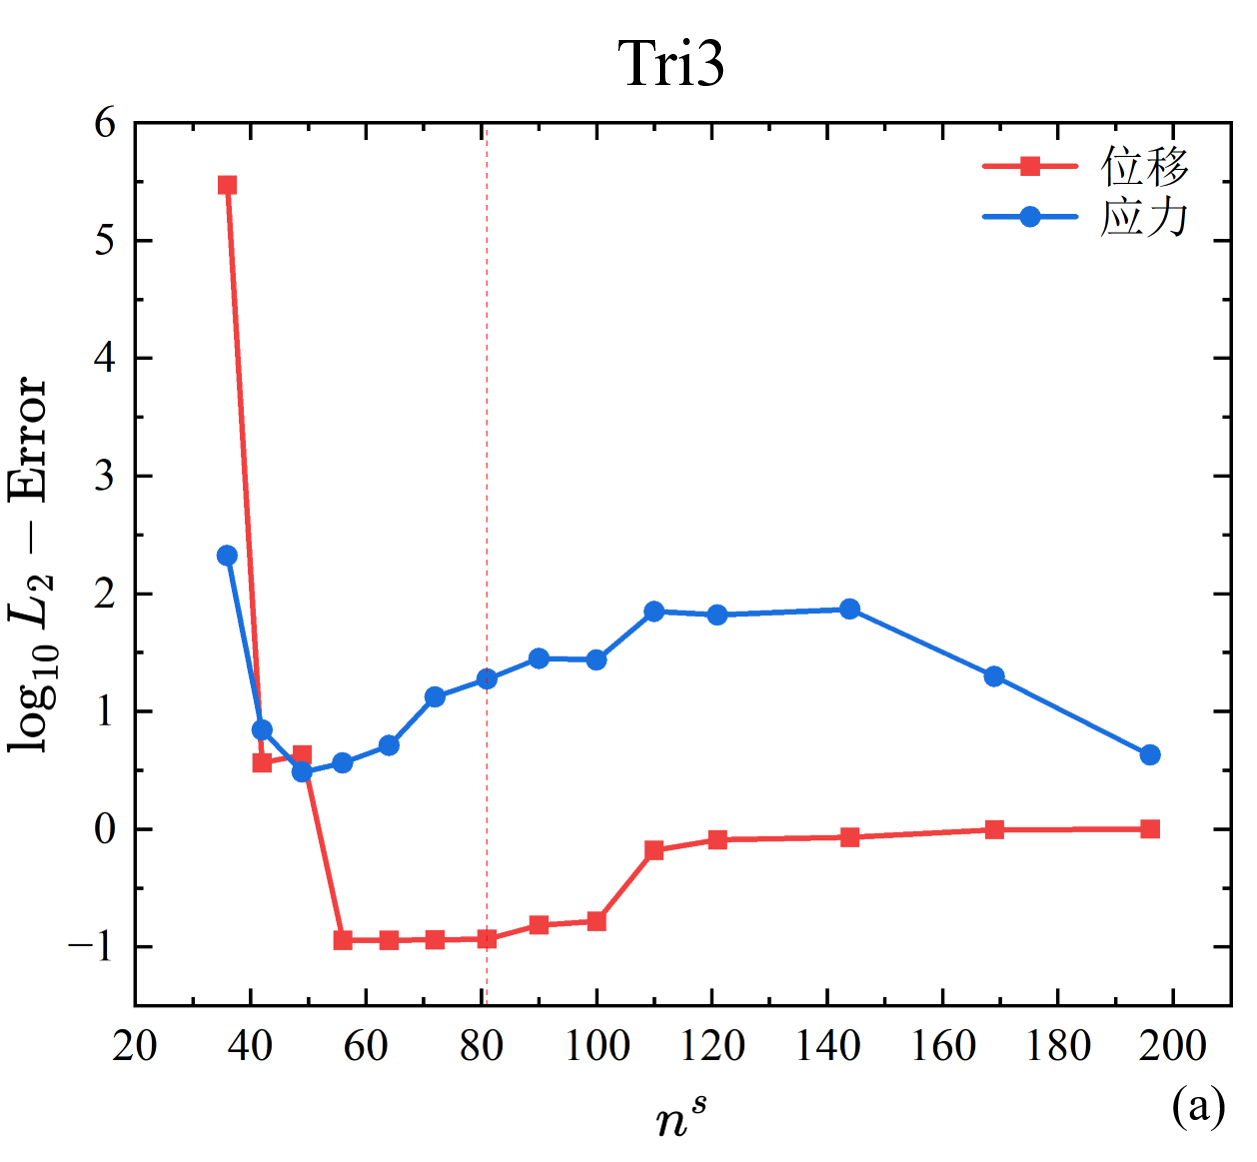
\includegraphics[width=0.48\textwidth]{figures/shearlocking/T3-l2-ns8.png}
    \phantomcaption\label{T3-l2-ns8}
    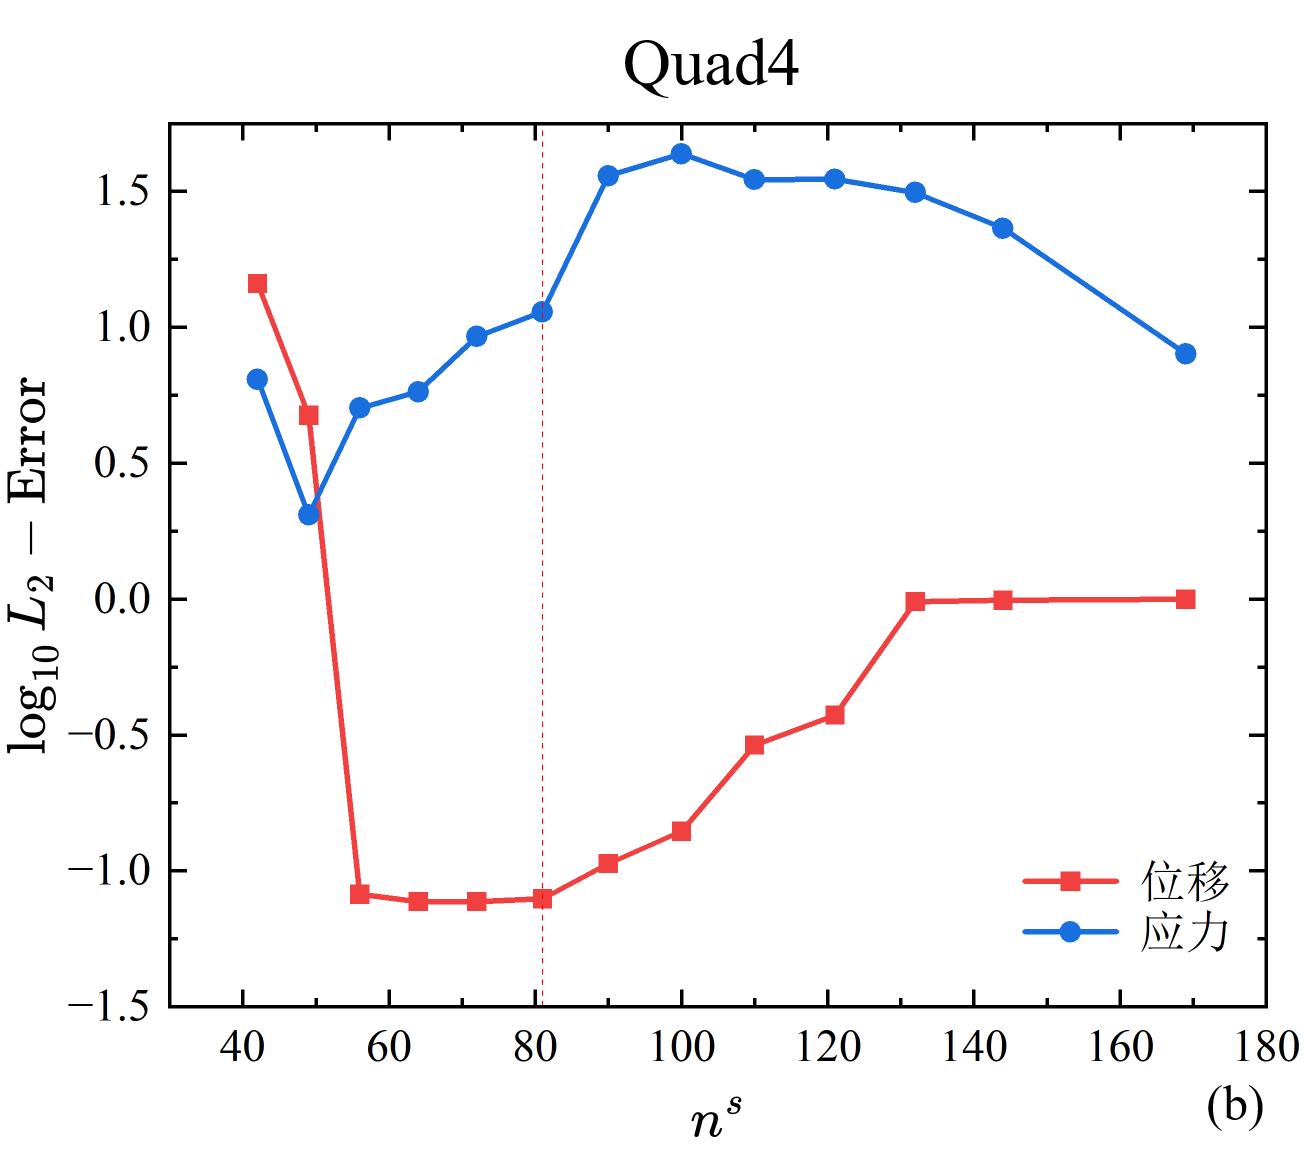
\includegraphics[width=0.50\textwidth]{figures/shearlocking/Q4-l2-ns8.png}
    \phantomcaption\label{Q4-l2-ns8}
    \end{subcaptiongroup}
    \begin{subcaptiongroup}
    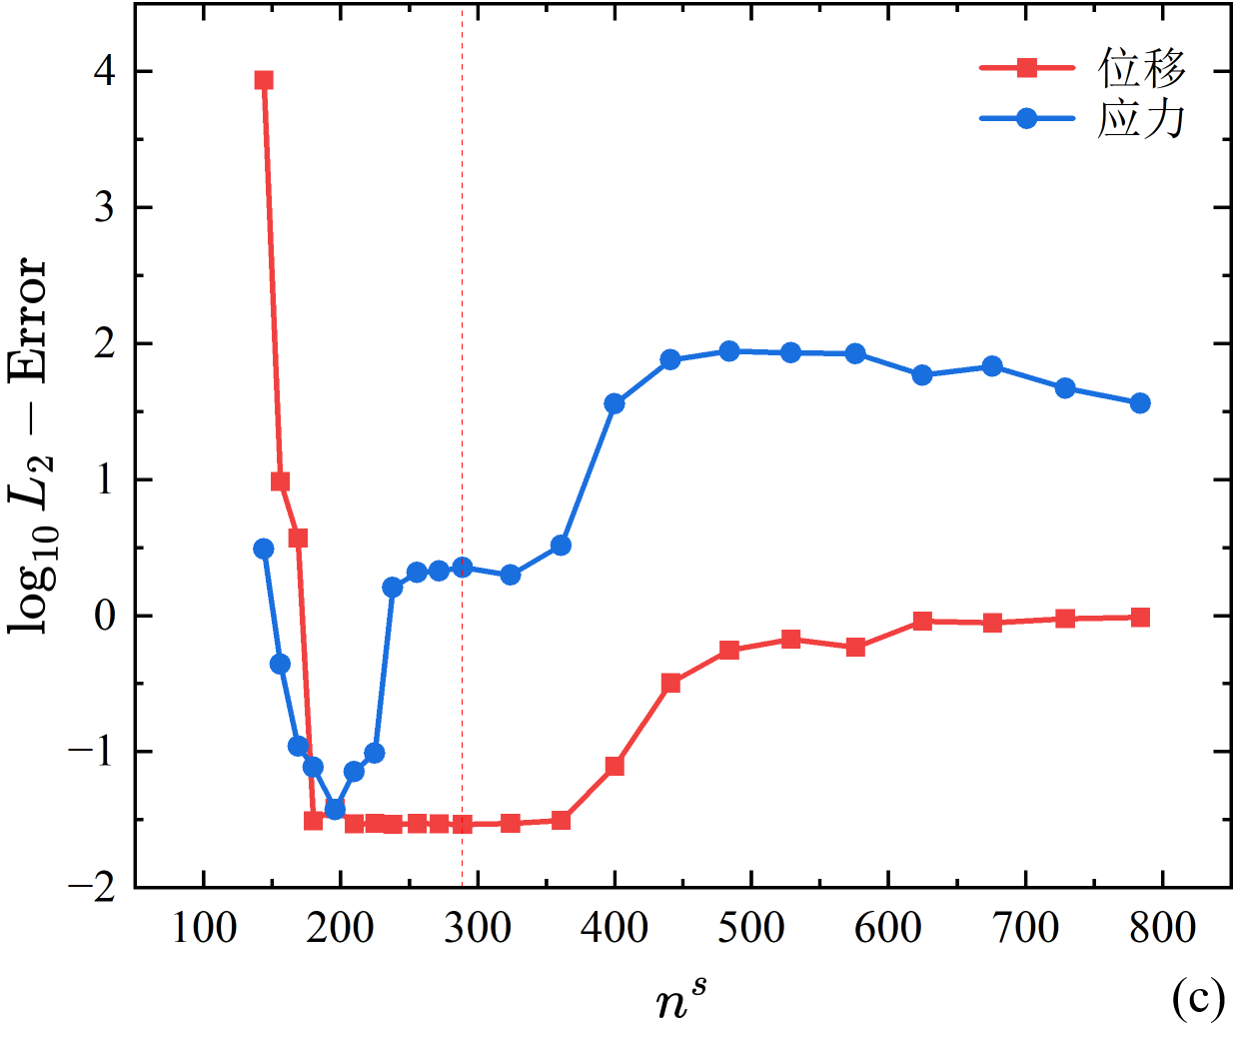
\includegraphics[width=0.49\textwidth]{figures/shearlocking/T3-l2-ns16.png}
    \phantomcaption\label{T3-l2-ns16}
    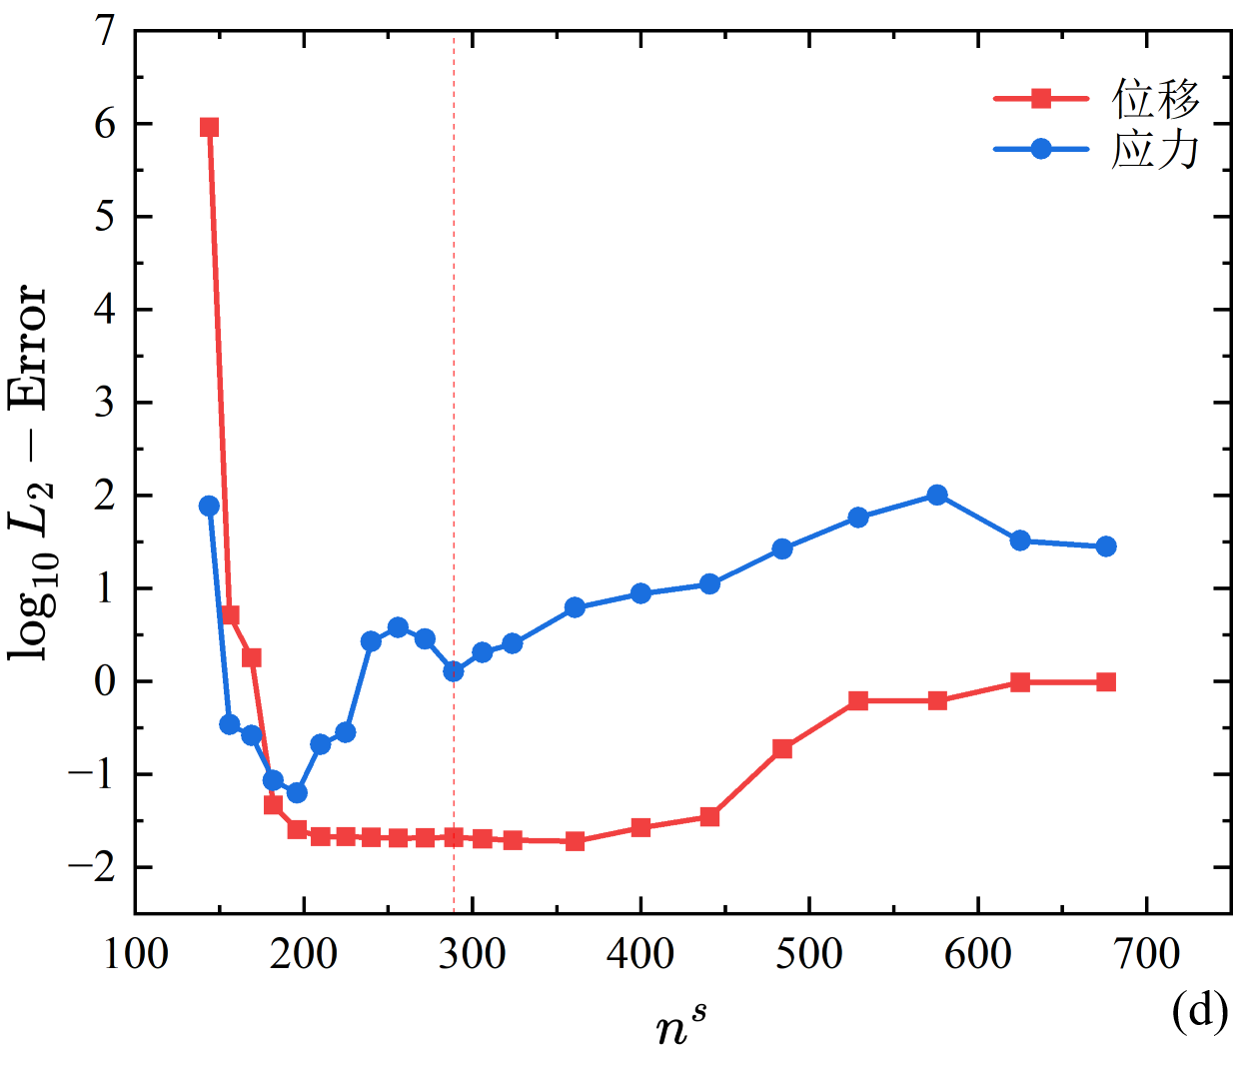
\includegraphics[width=0.49\textwidth]{figures/shearlocking/Q4-l2-ns16.png}
    \phantomcaption\label{Q4-l2-ns16}
    \end{subcaptiongroup}
    \begin{subcaptiongroup}
    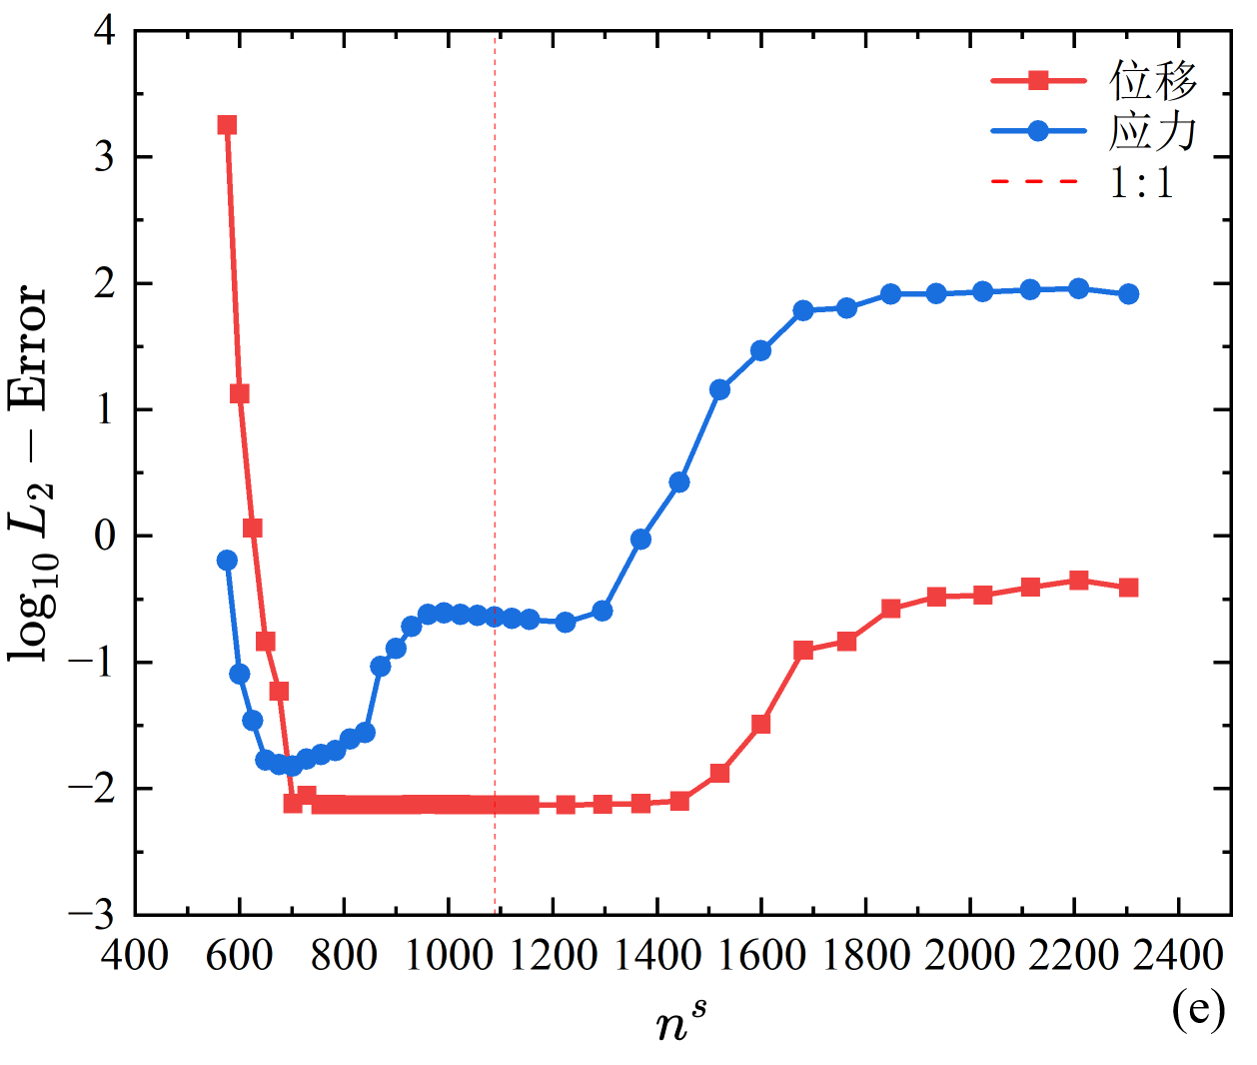
\includegraphics[width=0.49\textwidth]{figures/shearlocking/T3-l2-ns32.png}
    \phantomcaption\label{T3-l2-ns32}
    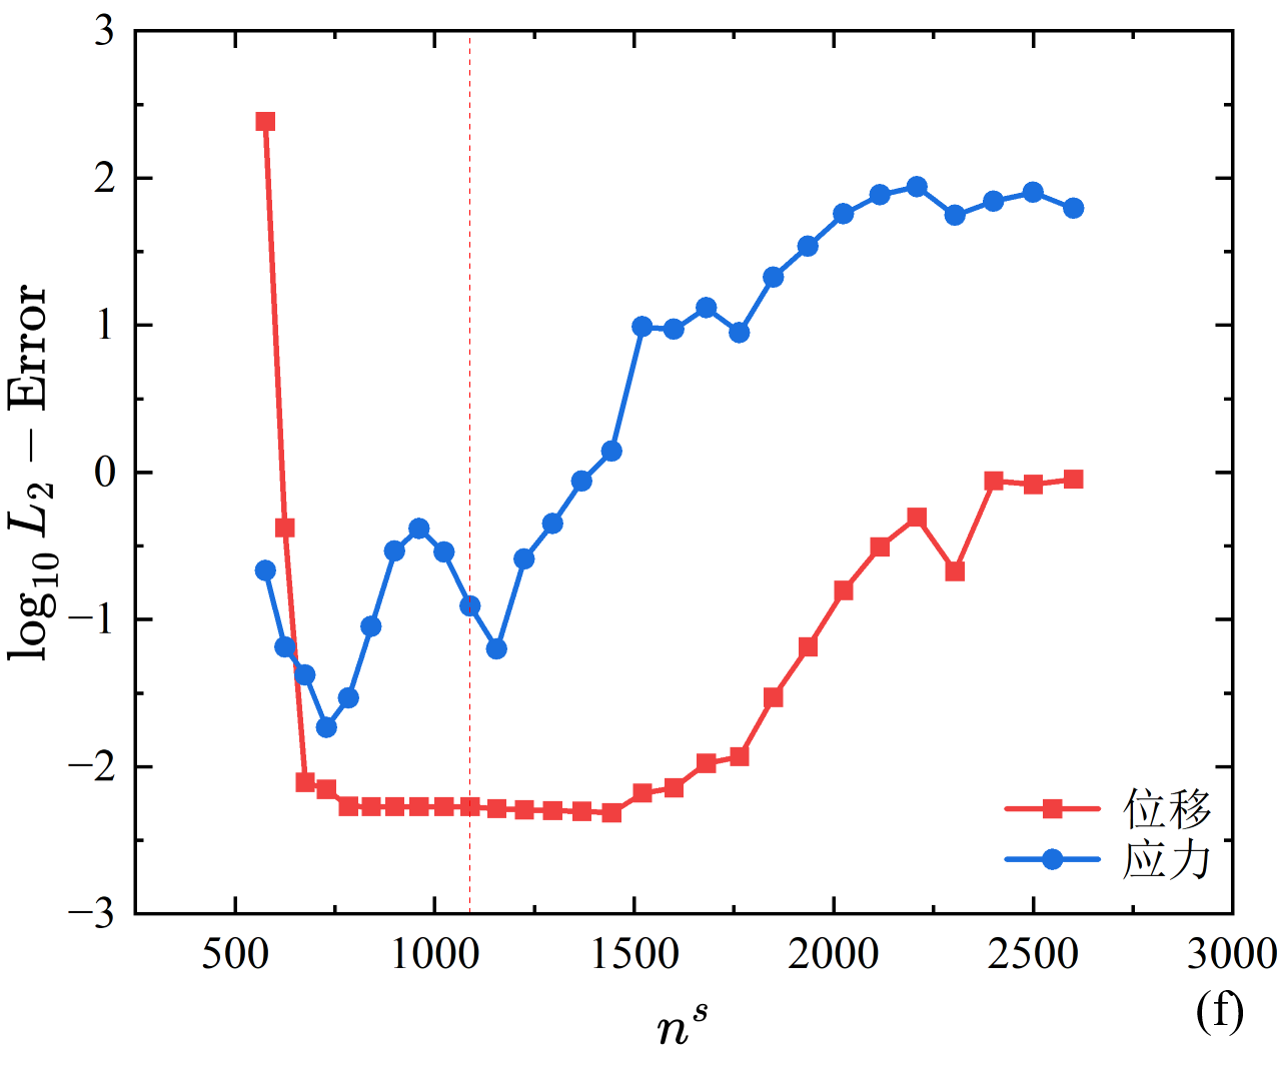
\includegraphics[width=0.49\textwidth]{figures/shearlocking/Q4-l2-ns32.png}
    \phantomcaption\label{Q4-l2-ns32}
    \end{subcaptiongroup}
\caption{\centering{固支方板问题线性单元$L2$误差与剪切应力节点数量的关系:\protect\linebreak
\subref{T3-l2-ns8},\subref{Q4-l2-ns8} $8\times 8$单元$L_2$误差; 
\subref{T3-l2-ns16},\subref{Q4-l2-ns16} $16\times 16$单元$L_2$误差;
\subref{T3-l2-ns32},\subref{Q4-l2-ns32} $32\times 32$单元$L_2$误差}}
\label{ch_5:fig:linear_ns}
\end{figure}

\begin{figure}[!h]
    \centering
    \begin{subcaptiongroup}
    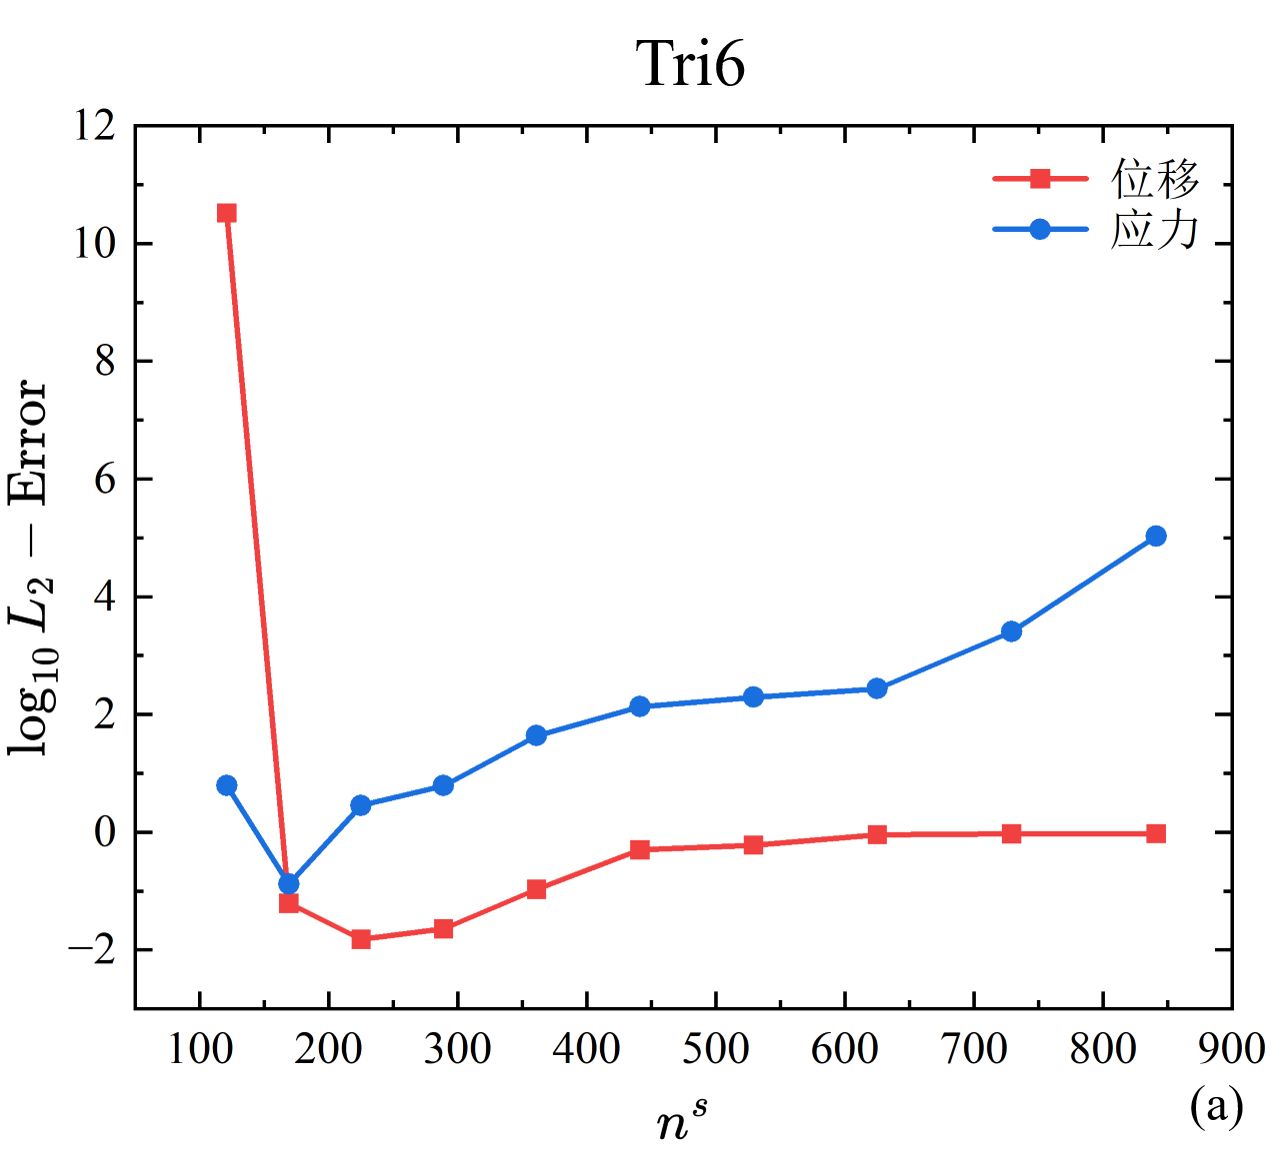
\includegraphics[width=0.49\textwidth]{figures/shearlocking/T6-l2-ns8.png}
    \phantomcaption\label{T6-l2-ns8}
    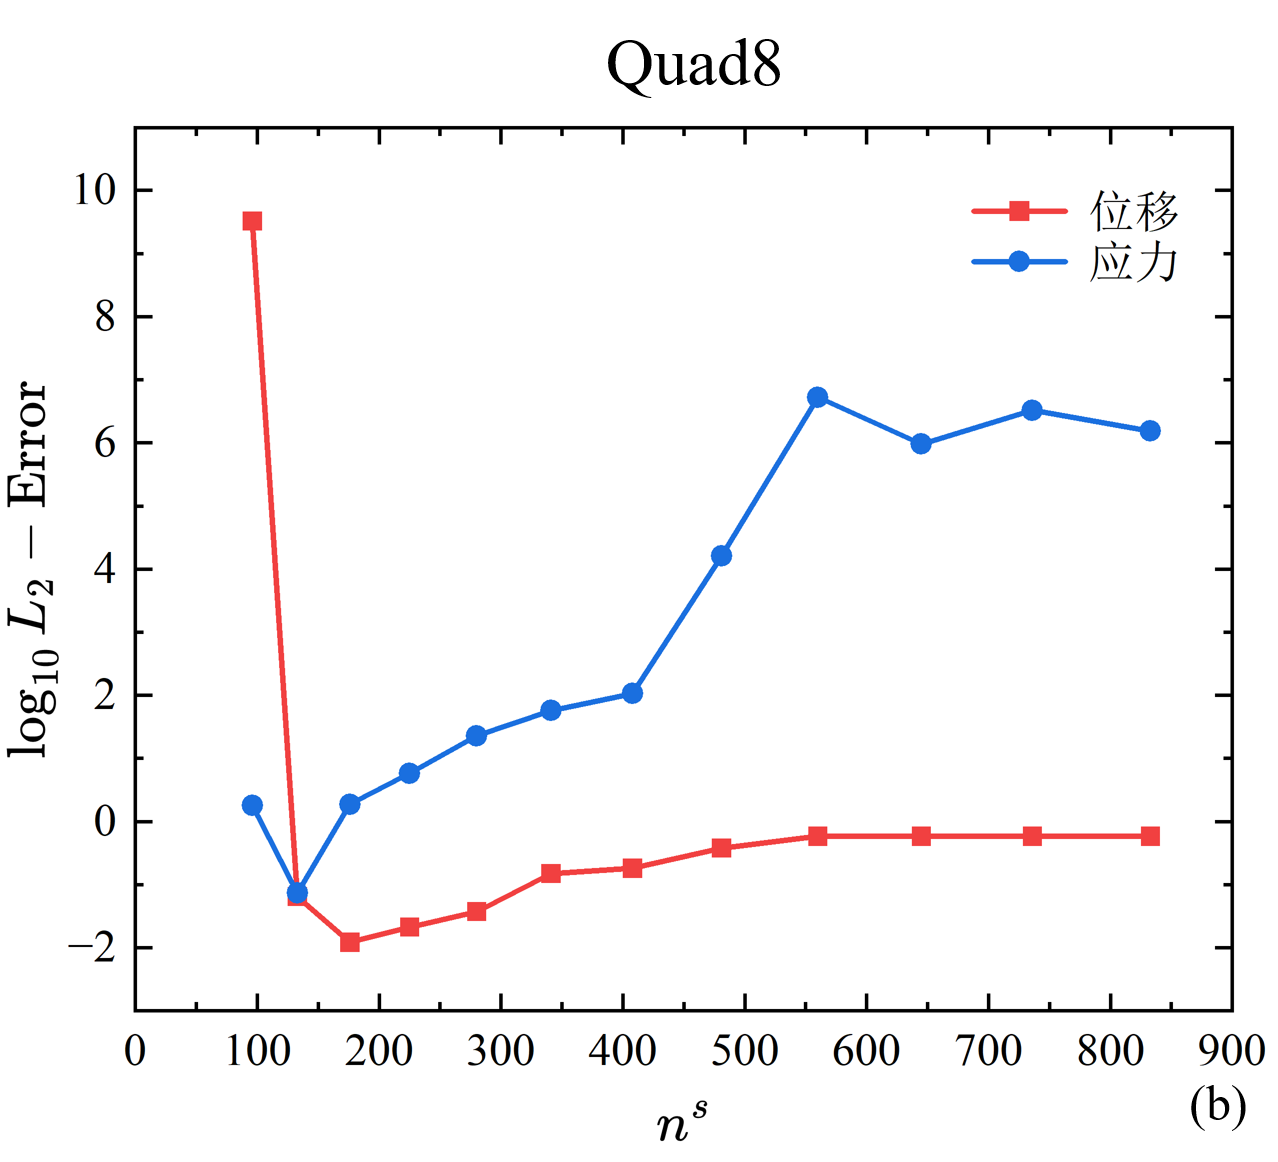
\includegraphics[width=0.49\textwidth]{figures/shearlocking/Q8-l2-ns8.png}
    \phantomcaption\label{Q8-l2-ns8}
    \end{subcaptiongroup}
    \begin{subcaptiongroup}
    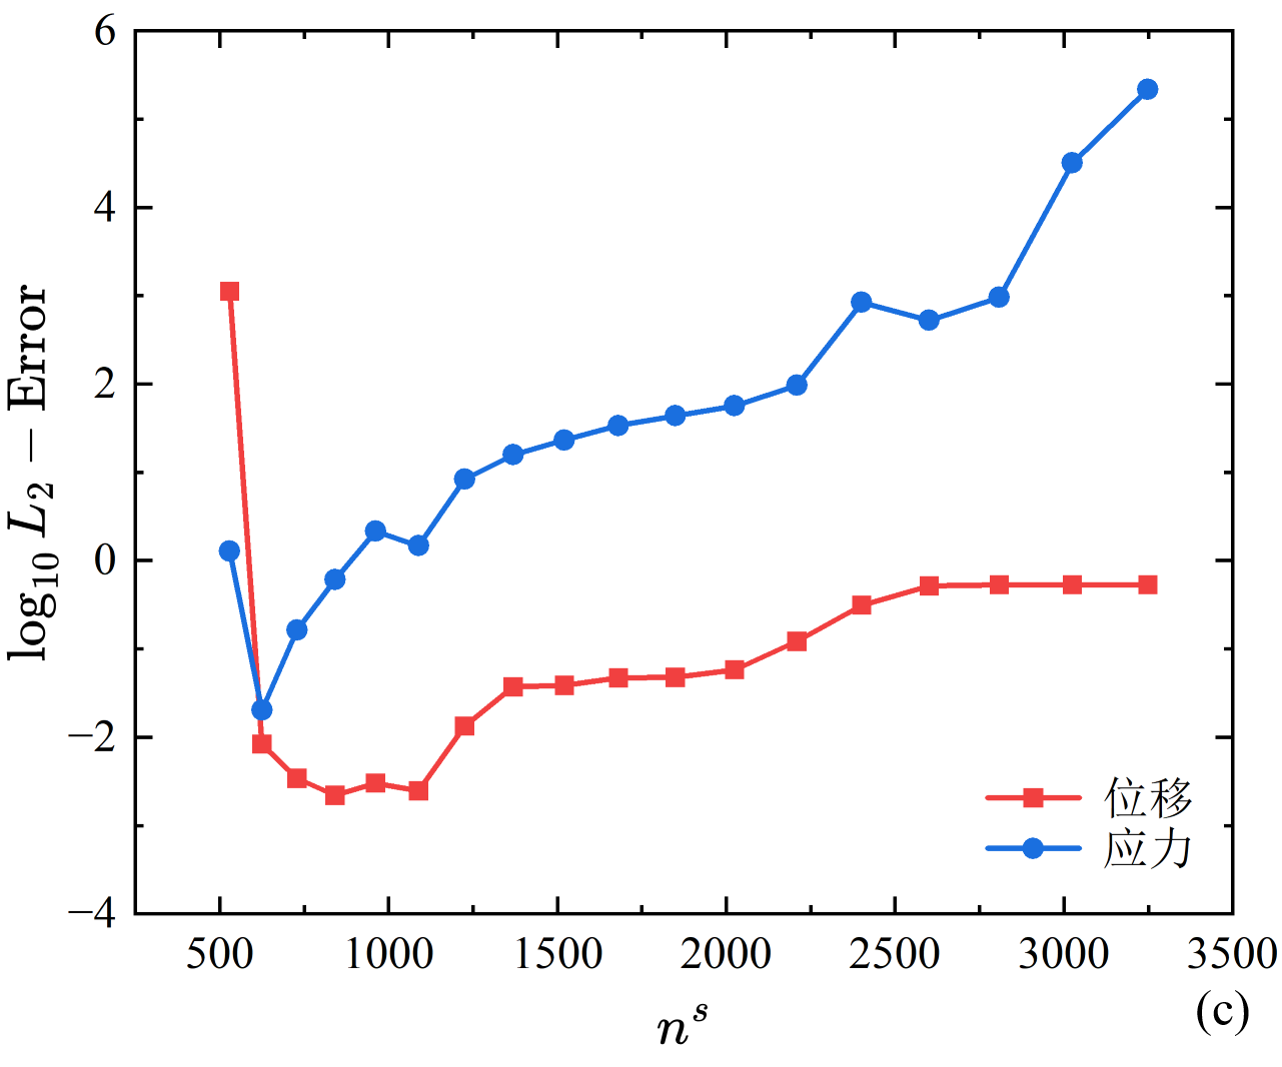
\includegraphics[width=0.49\textwidth]{figures/shearlocking/T6-l2-ns16.png}
    \phantomcaption\label{T6-l2-ns16}
    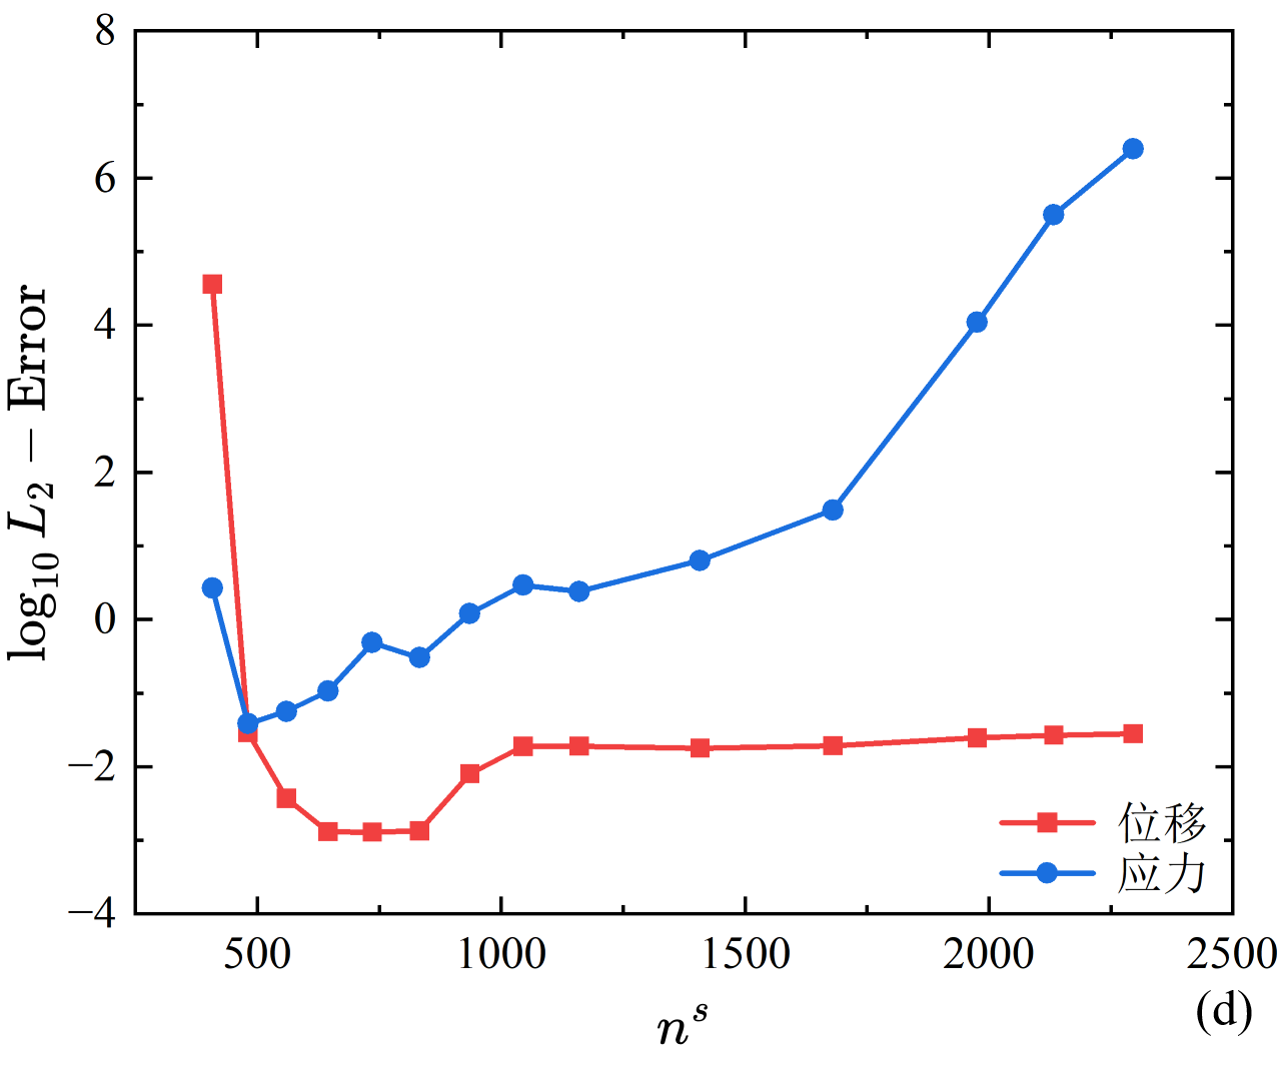
\includegraphics[width=0.49\textwidth]{figures/shearlocking/Q8-l2-ns16.png}
    \phantomcaption\label{Q8-l2-ns16}
    \end{subcaptiongroup}
    \begin{subcaptiongroup}
    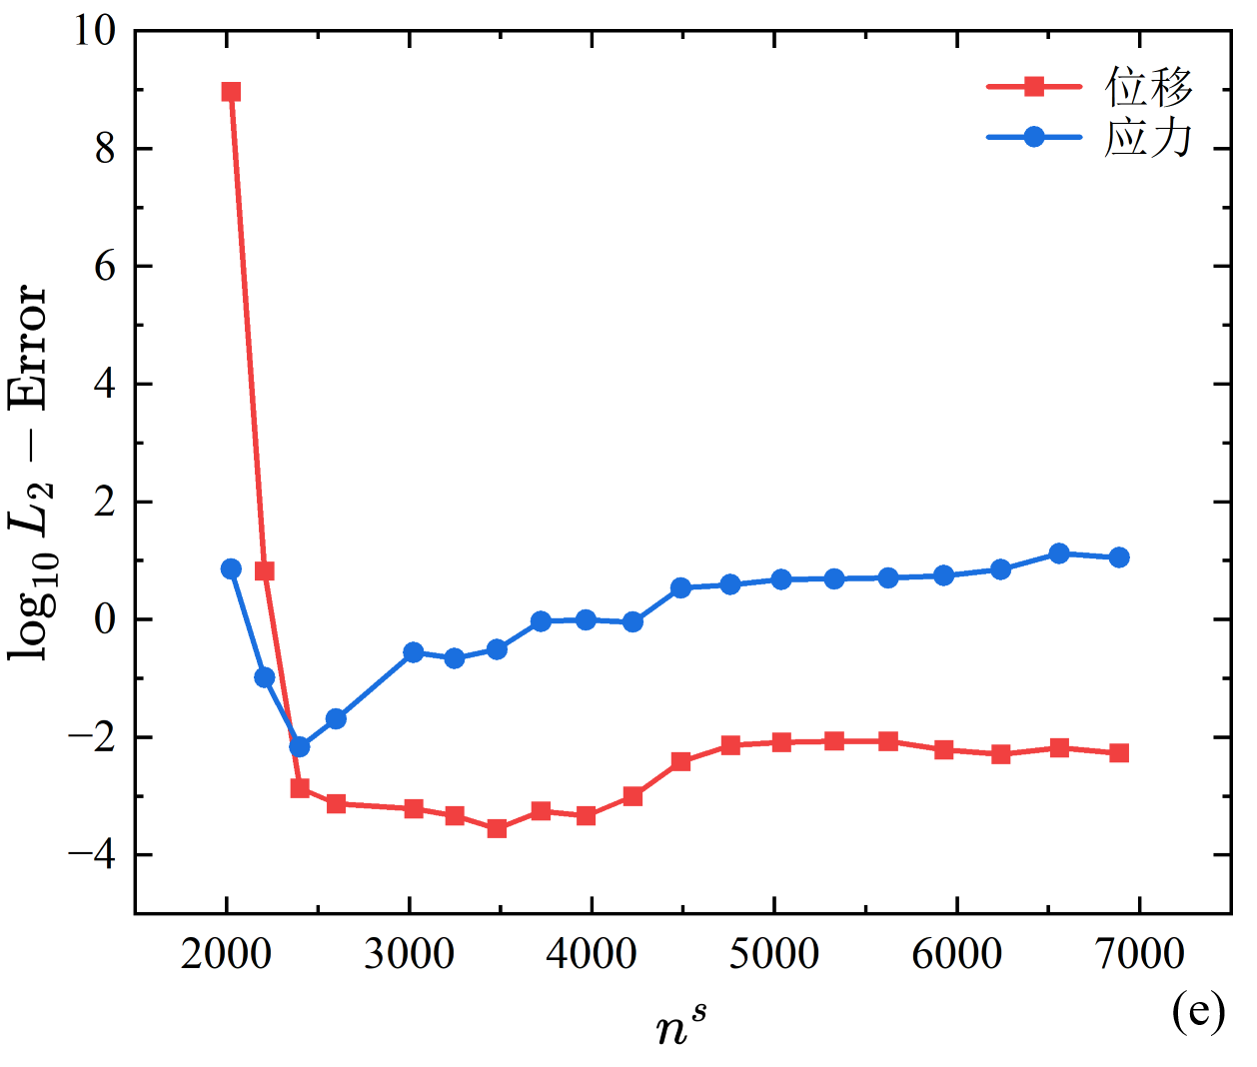
\includegraphics[width=0.49\textwidth]{figures/shearlocking/T6-l2-ns32.png}
    \phantomcaption\label{T6-l2-ns32}
    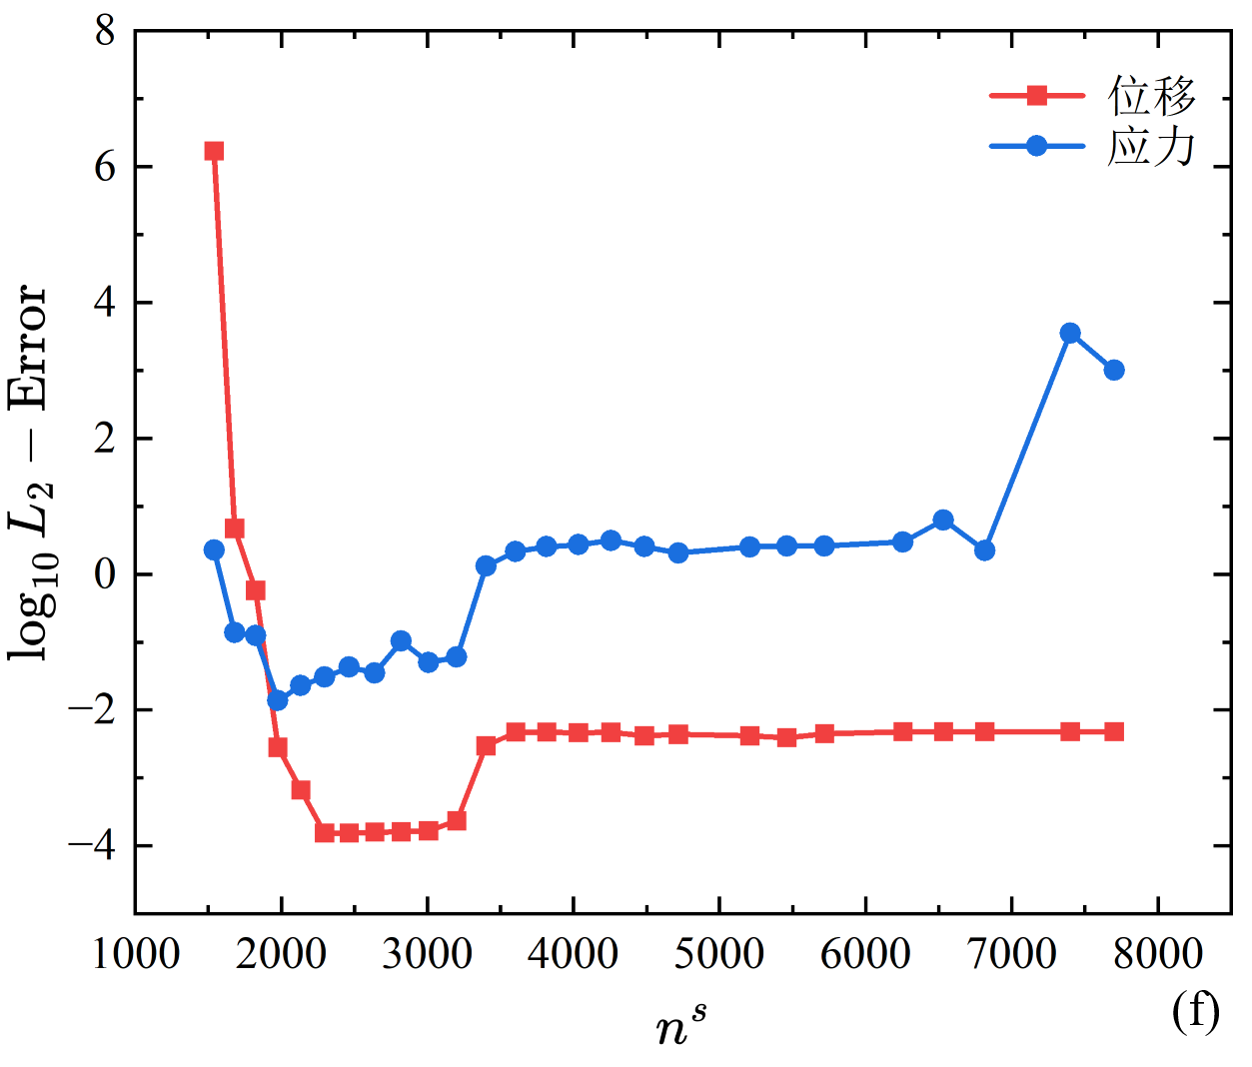
\includegraphics[width=0.49\textwidth]{figures/shearlocking/Q8-l2-ns32.png}
    \phantomcaption\label{Q8-l2-ns32}
    \end{subcaptiongroup}
\caption{\centering{固支方板问题二次单元$L2$误差与剪切应力节点数量的关系:\protect\linebreak 
\subref{T6-l2-ns8},\subref{Q8-l2-ns8} $8\times 8$单元$L_2$误差; 
\subref{T6-l2-ns16},\subref{Q8-l2-ns16} $16\times 16$单元$L_2$误差;
\subref{T6-l2-ns32},\subref{Q8-l2-ns32} $32\times 32$单元$L_2$误差}}
\label{ch_5:fig:quad_ns}
\end{figure}

分析固支方板问题的应力精确解云图\ref{ch_5:fig:plate_exact_solution},可以观察到应力$Q_1$、$Q_2$具有相似的性质。在进一步的研究中仅针对
$Q_1$进行探讨。如图\ref{ch_5:fig:Q1_Tri3}对于Tri3单元,在不同位移节点数量下,传统约束比例与最优约束比例的应力云图存在显著的差异。当节点
数量按照传统约束比例设置时,会出现明显的应力振荡现象。随着位移节点的增加这种应力振荡现象有所的缓解,但仍然存在。相较之下,在最优
约束比下没有发生应力振荡现象。Quad4单元的应力云图\ref{ch_5:fig:Q1_Quad4}和Quad8单元图\ref{ch_5:fig:Q1_Quad8}也表现出类似的现象。对于Tri6单元
图\ref{ch_5:fig:Q1_Tri6}而言,即使位移节点增加,节点数量按照传统约束比设置时,始终会出现应力振荡现象,而最优约束比例时没有发生应力振荡现象。
\begin{figure}[!h]
    \centering
    \begin{subcaptiongroup}
    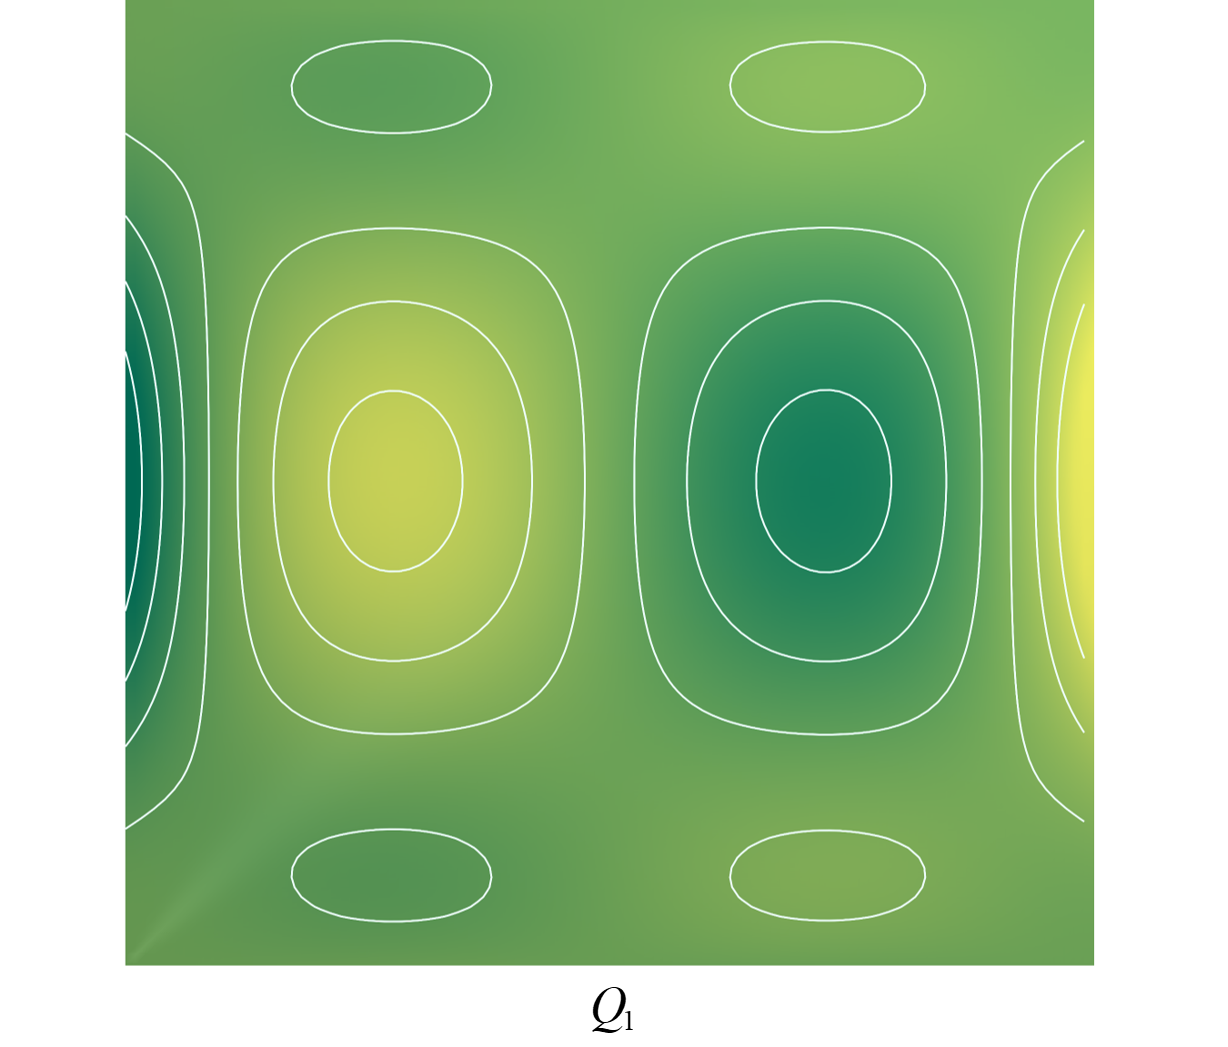
\includegraphics[width=0.46\textwidth]{figures/shearlocking/plate_exactQ1_solution.png}
    \phantomcaption
    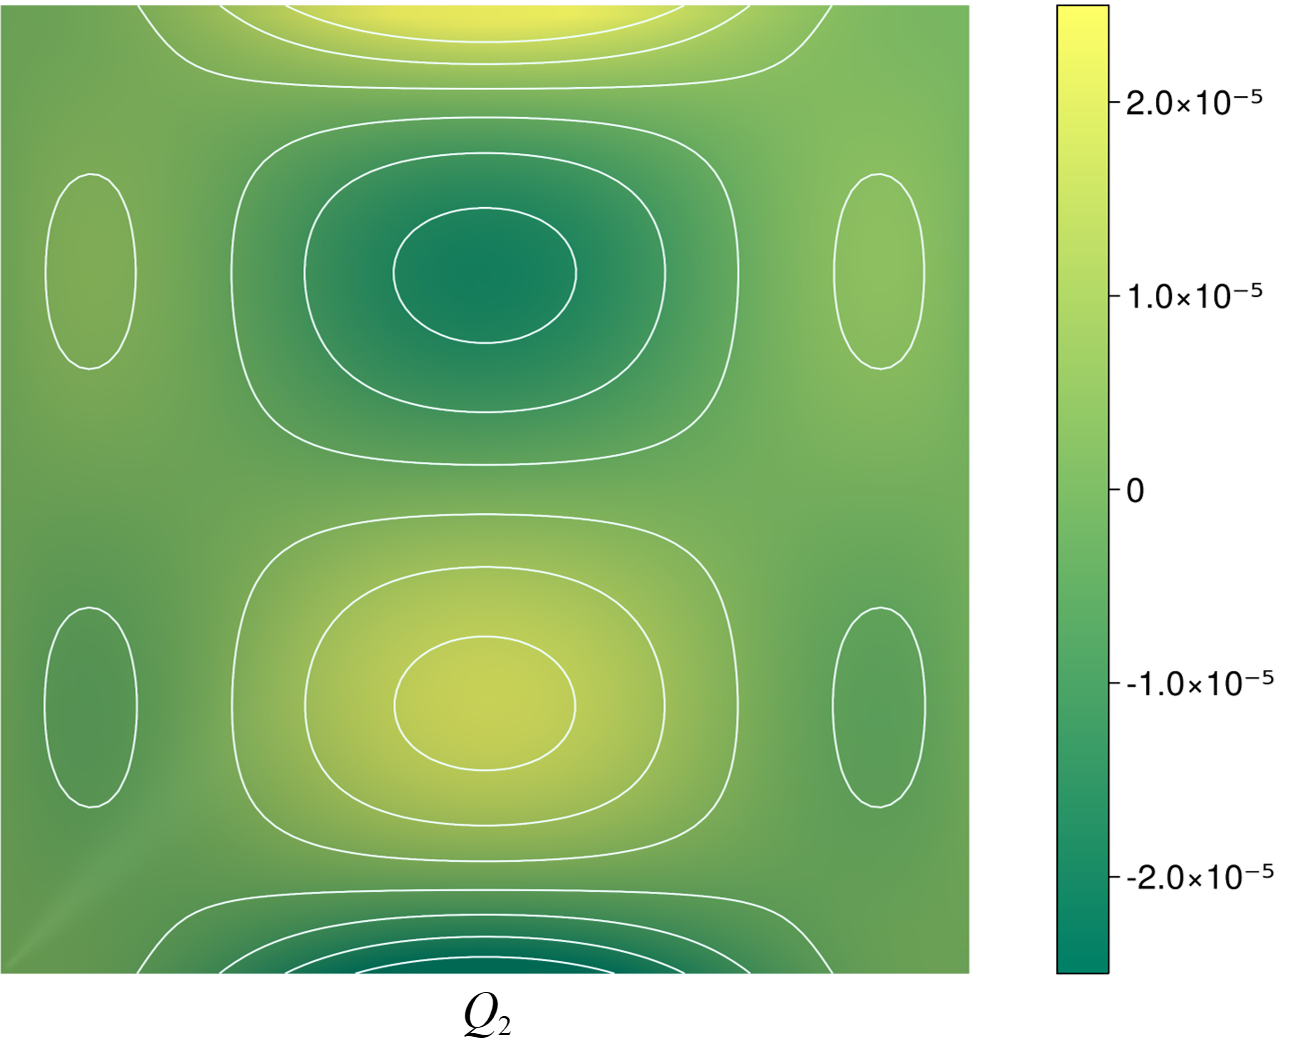
\includegraphics[width=0.49\textwidth]{figures/shearlocking/plate_exactQ2_solution.png}
    \phantomcaption
    \end{subcaptiongroup}
\caption{\centering{固支方板问题应力精确解}}
\label{ch_5:fig:plate_exact_solution}
\end{figure}


\begin{figure}[!h]
    \centering
    \begin{tabular}{cccc}
    $\quad$&最优约束比&传统约束比\\
    $81$&\begin{subcaptiongroup}\raisebox{-0.5\height}{\includegraphics[width=0.4\textwidth]{figures/shearlocking/SquarePlate_T3_q1_8_7.png}}\end{subcaptiongroup}
    &\begin{subcaptiongroup}\raisebox{-0.5\height}{\includegraphics[width=0.4\textwidth]{figures/shearlocking/SquarePlate_T3_q1_8_8.png}}\end{subcaptiongroup}\\
    $289$&\begin{subcaptiongroup}\raisebox{-0.5\height}{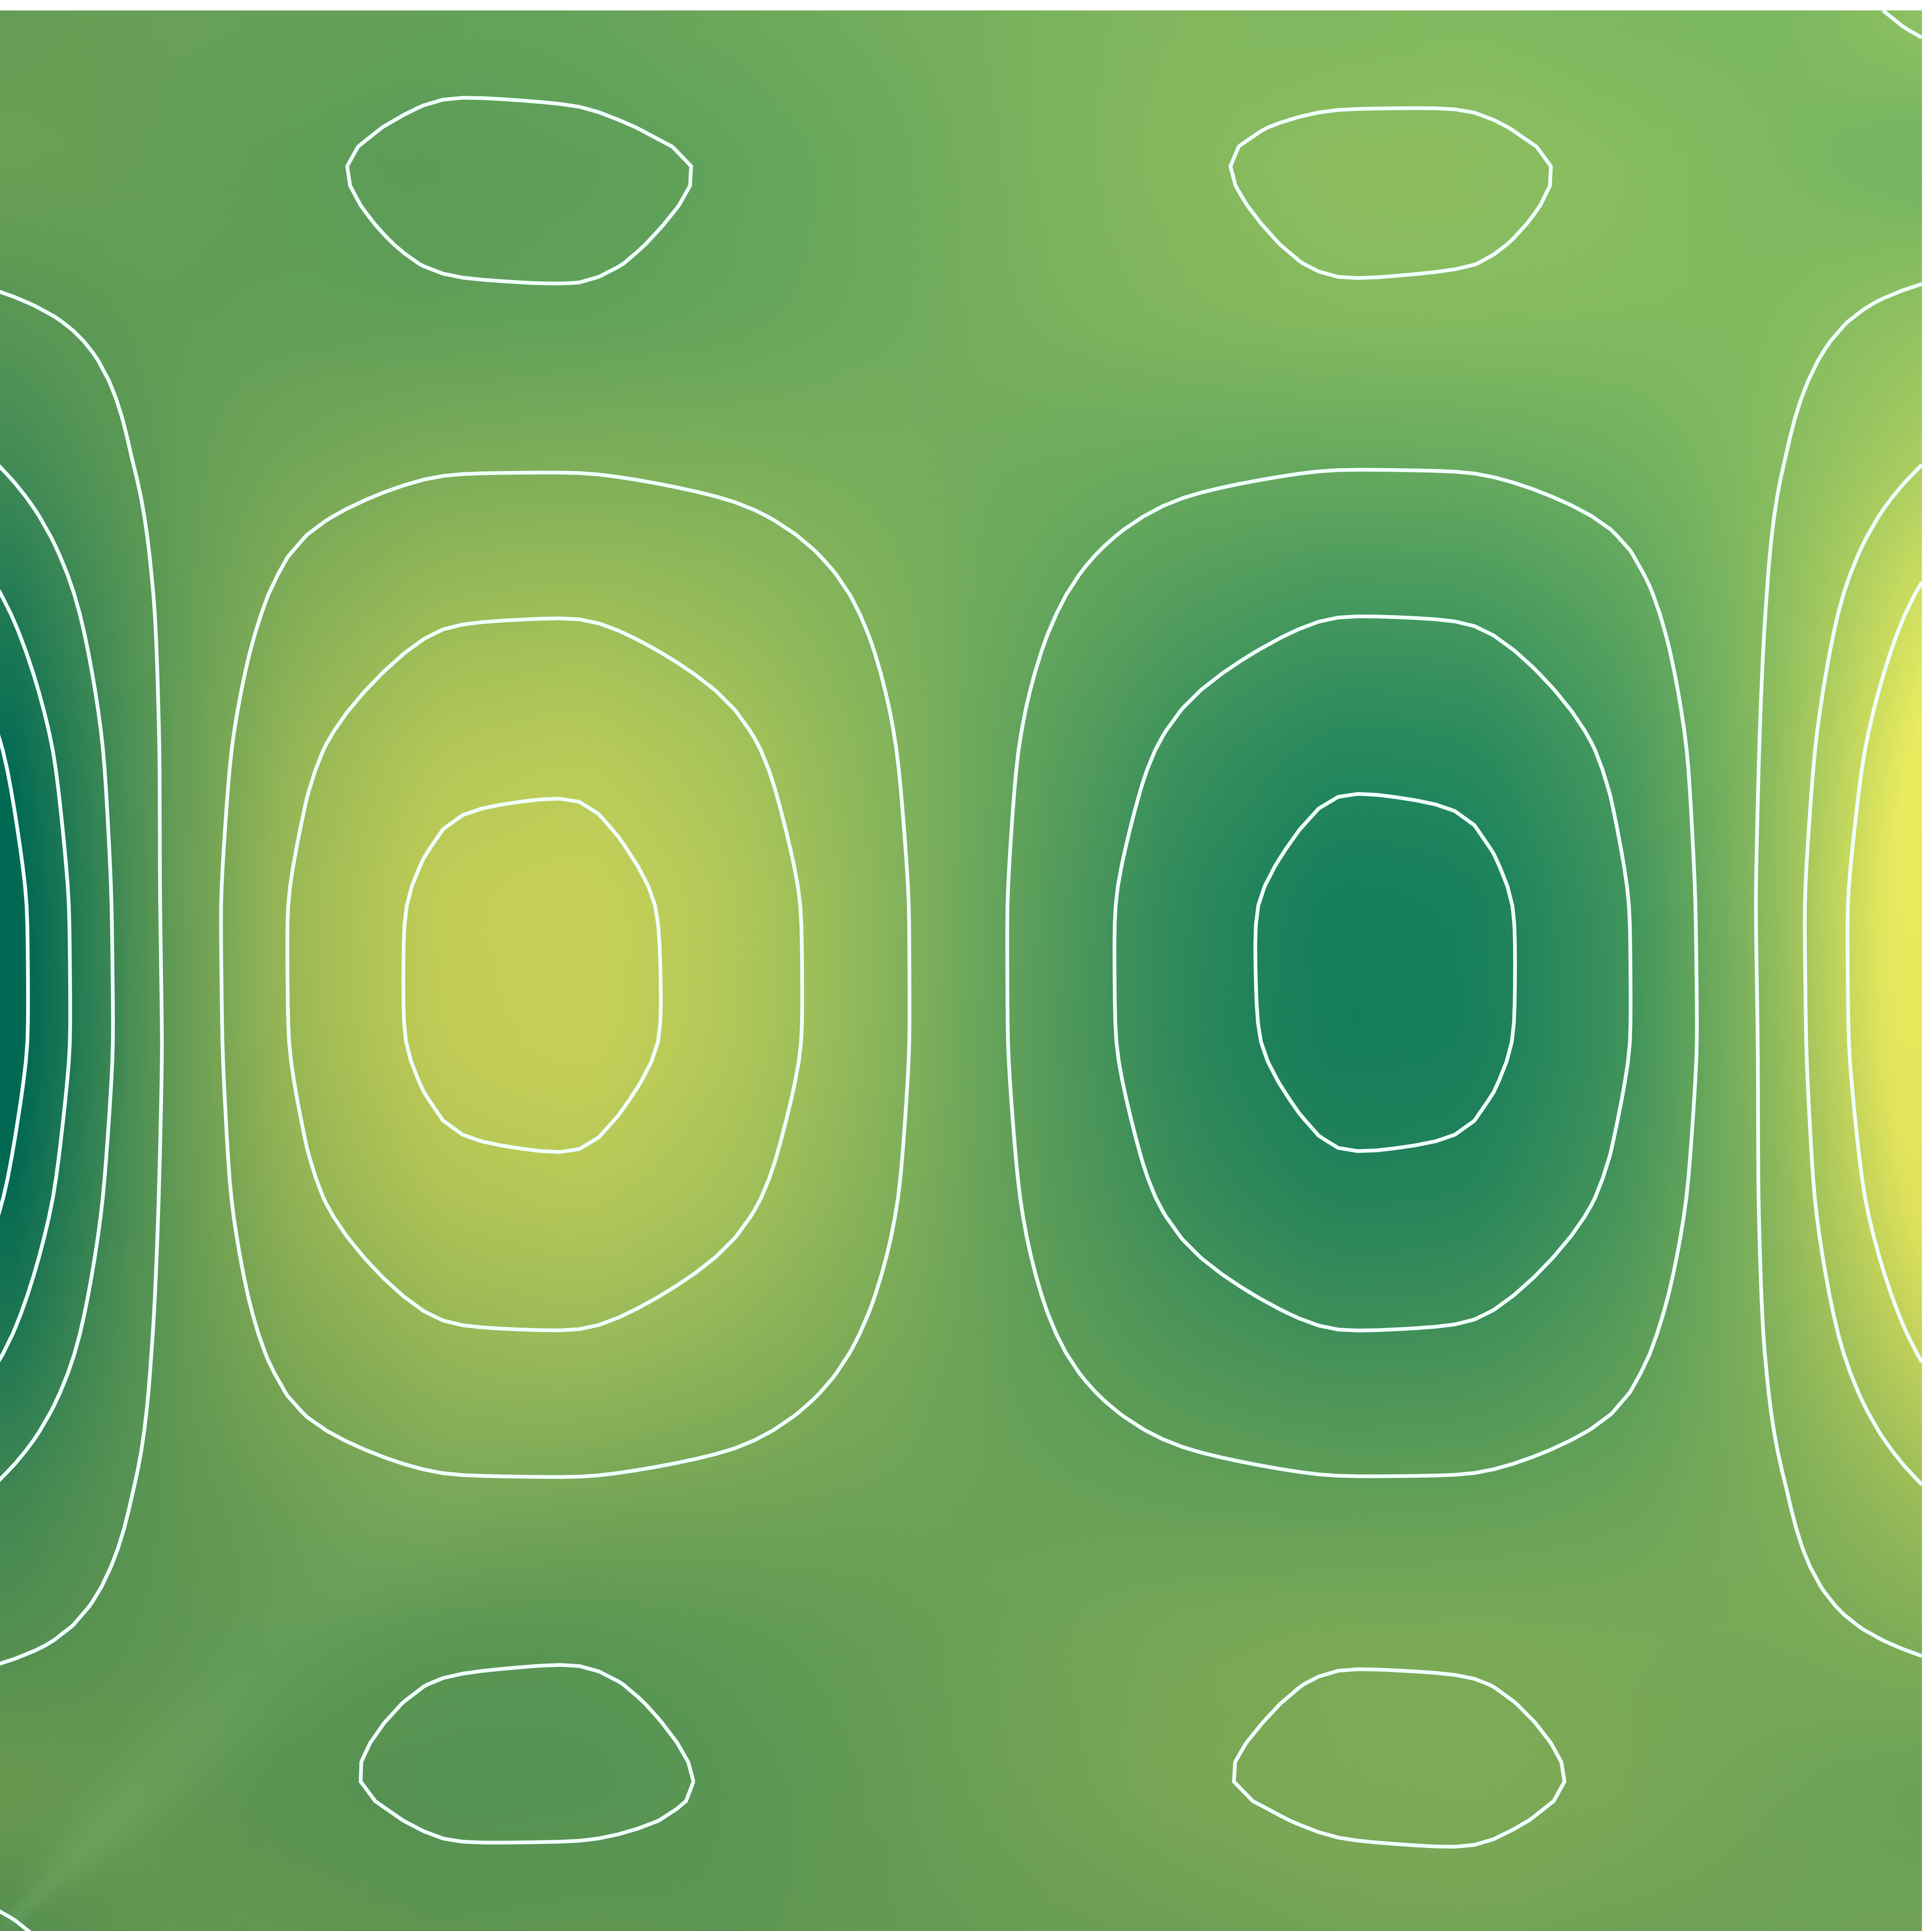
\includegraphics[width=0.4\textwidth]{figures/shearlocking/SquarePlate_T3_q1_16_13.png}}\end{subcaptiongroup}
    &\begin{subcaptiongroup}\raisebox{-0.5\height}{\includegraphics[width=0.4\textwidth]{figures/shearlocking/SquarePlate_T3_q1_16_16.png}}\end{subcaptiongroup}\\
    $1089$&\begin{subcaptiongroup}\raisebox{-0.5\height}{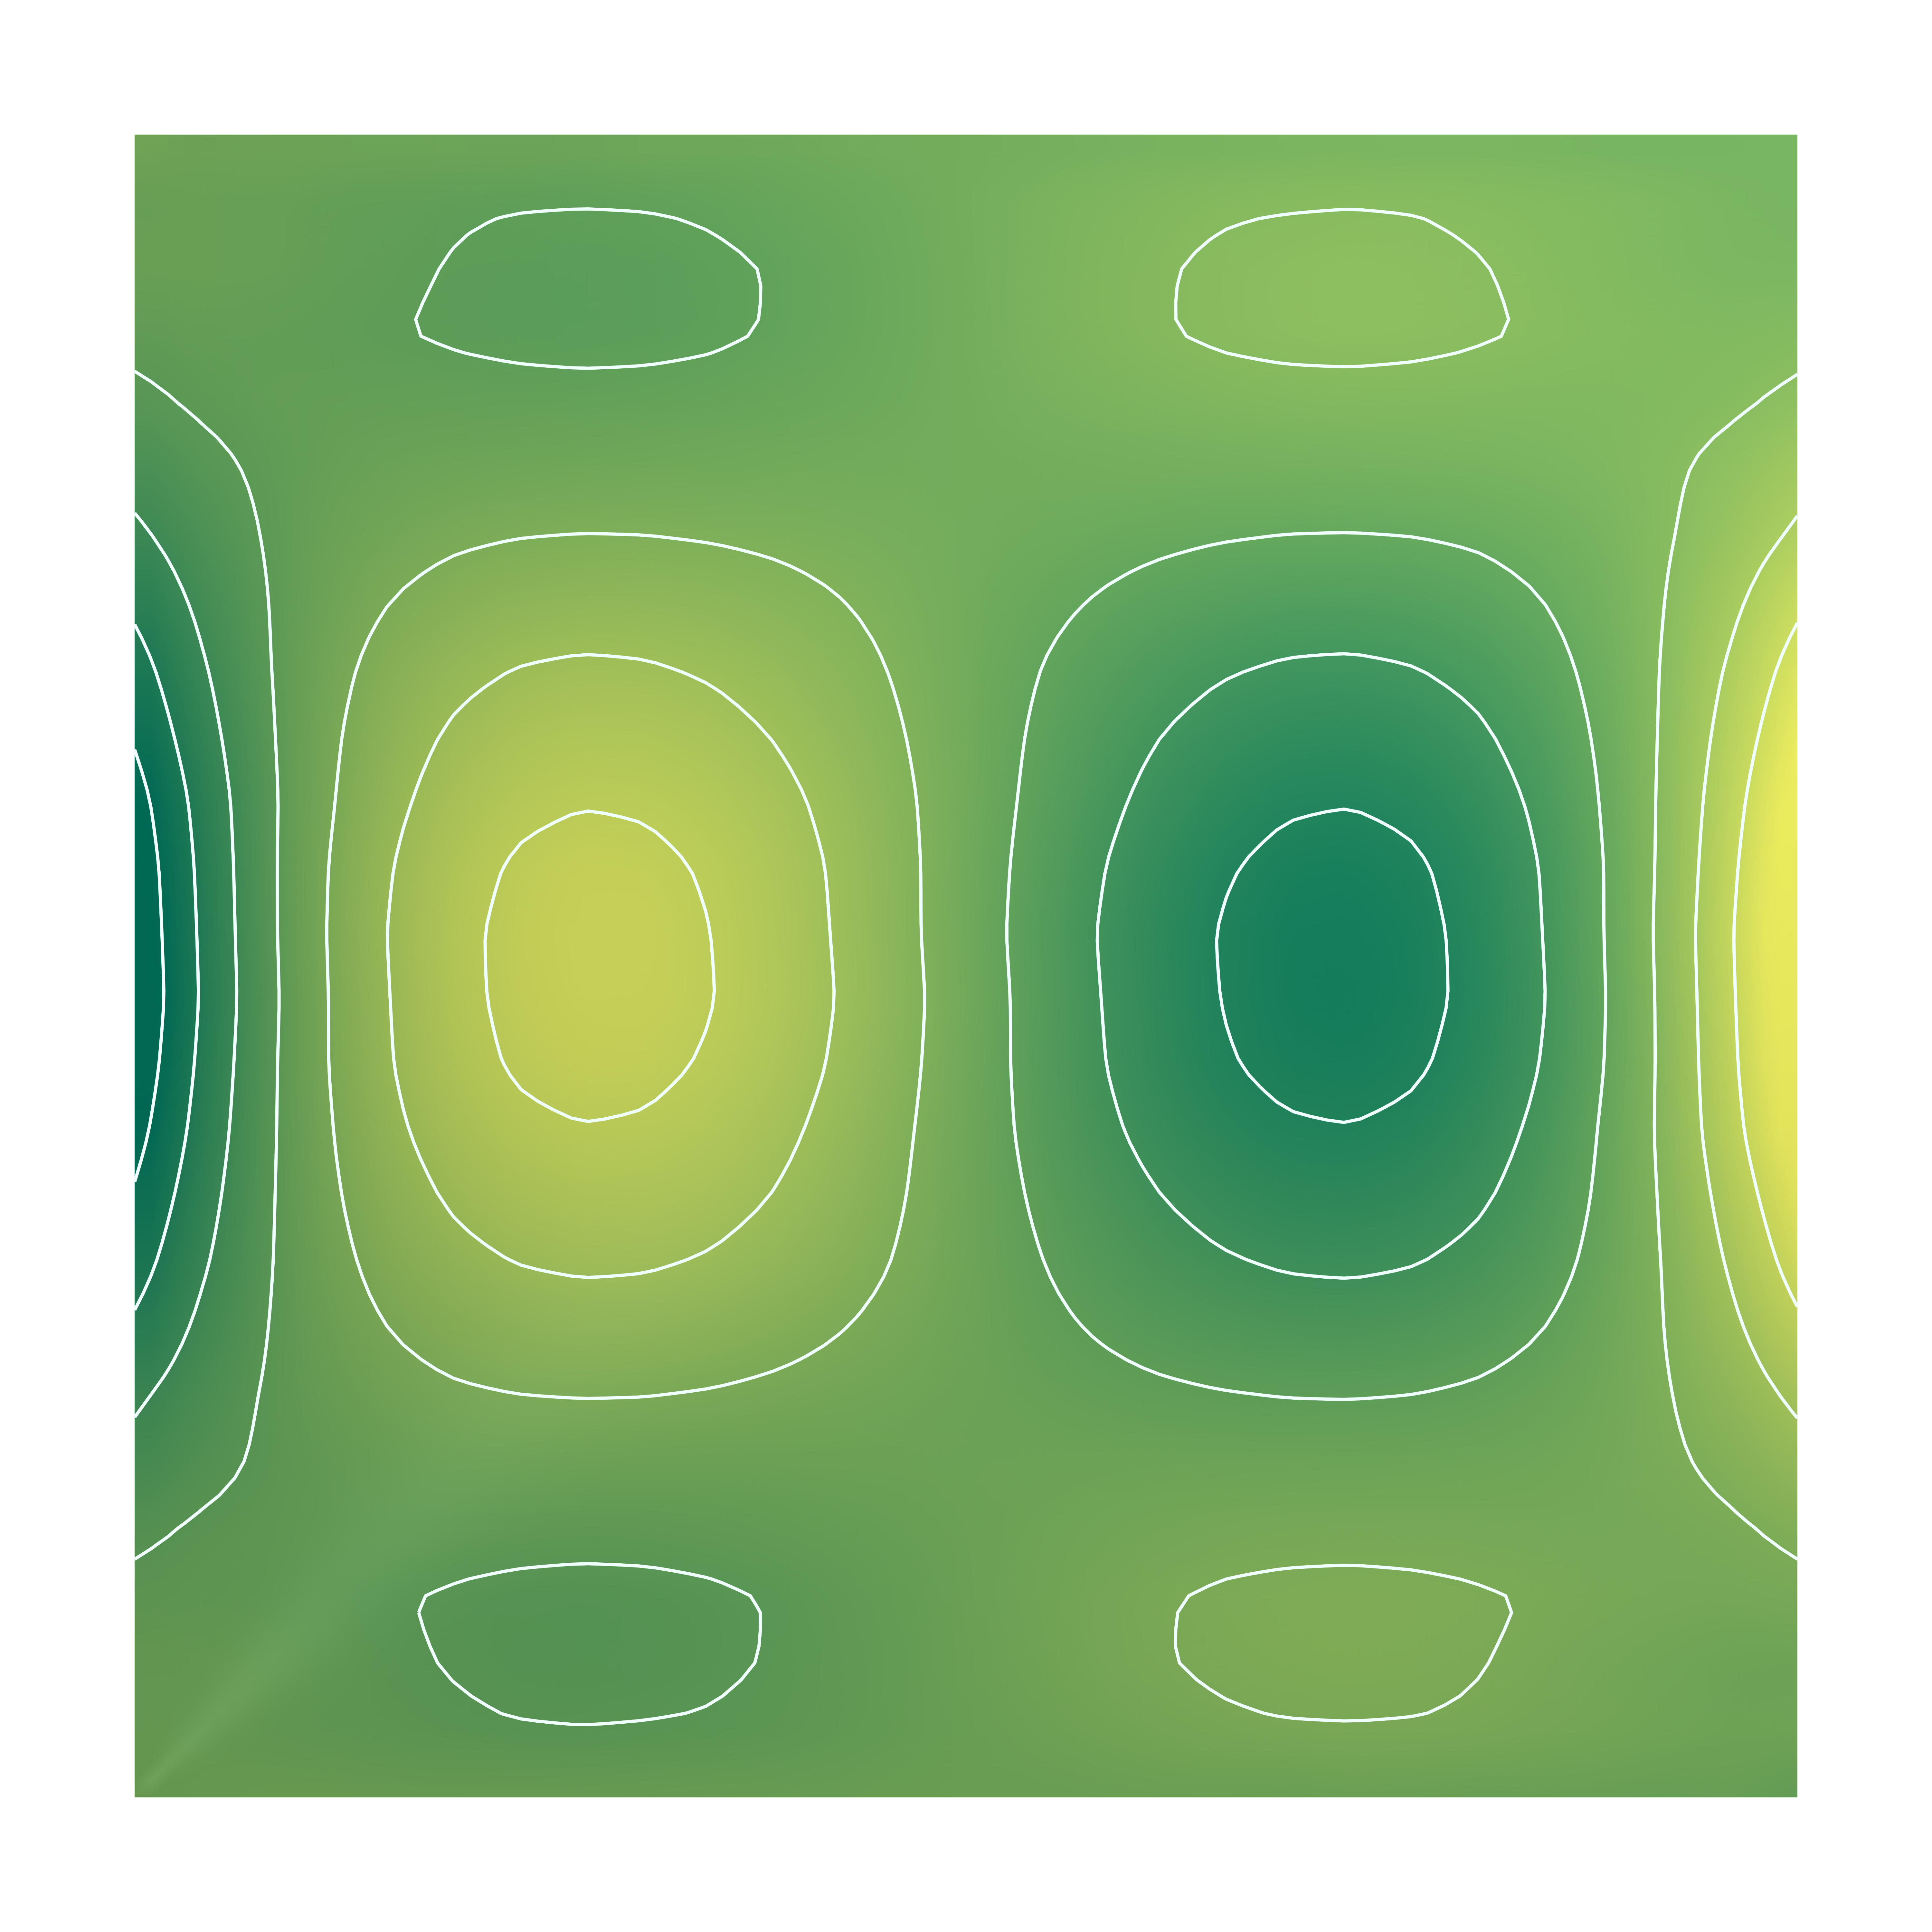
\includegraphics[width=0.4\textwidth]{figures/shearlocking/SquarePlate_T3_q1_32_26.png}}\end{subcaptiongroup}
    &\begin{subcaptiongroup}\raisebox{-0.5\height}{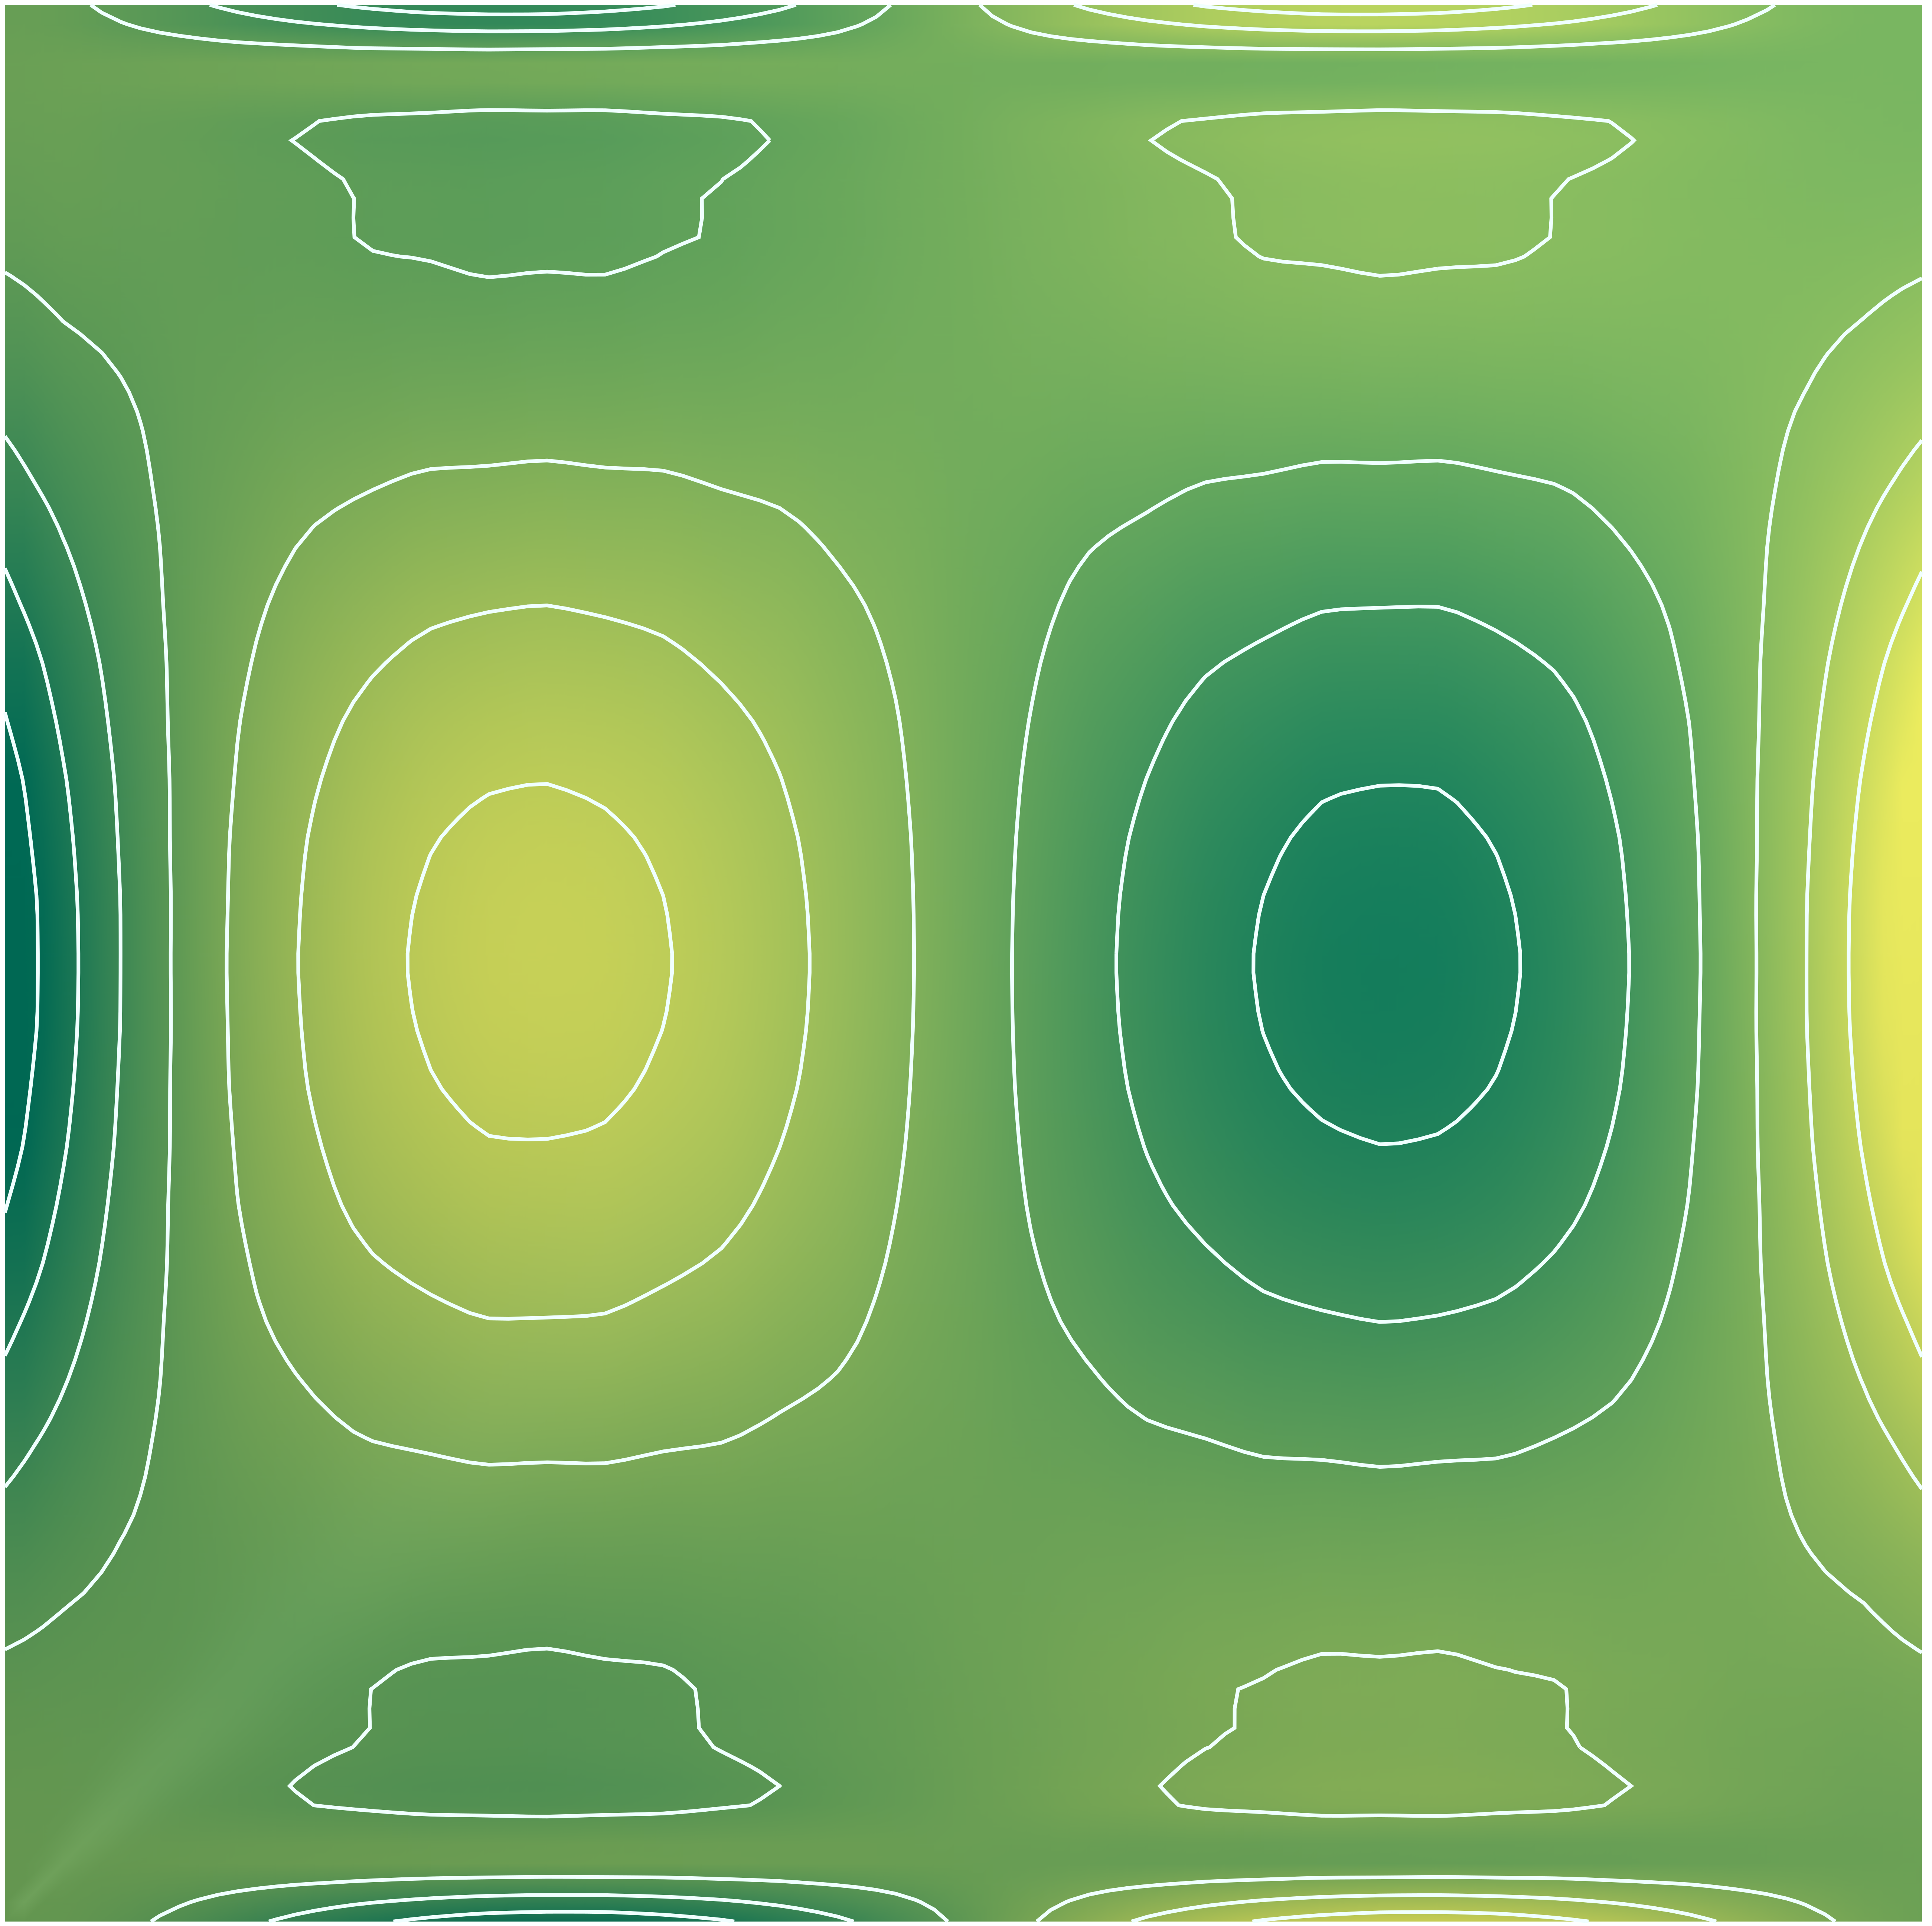
\includegraphics[width=0.4\textwidth]{figures/shearlocking/SquarePlate_T3_q1_32_32.png}}\end{subcaptiongroup}\\
    \end{tabular}
    \caption{\textbf{固支方板问题Tri3单元应力云图($Q_1$)}}\label{ch_5:fig:Q1_Tri3}
\end{figure}

\begin{figure}[!h]
    \centering
    \begin{tabular}{cccc}
    $\quad$&最优约束比&传统约束比\\
    $81$&\begin{subcaptiongroup}\raisebox{-0.5\height}{\includegraphics[width=0.4\textwidth]{figures/shearlocking/SquarePlate_mix_quad4_q1_8_7.png}}\end{subcaptiongroup}
    &\begin{subcaptiongroup}\raisebox{-0.5\height}{\includegraphics[width=0.4\textwidth]{figures/shearlocking/SquarePlate_mix_quad4_q1_8_8.png}}\end{subcaptiongroup}\\
    $289$&\begin{subcaptiongroup}\raisebox{-0.5\height}{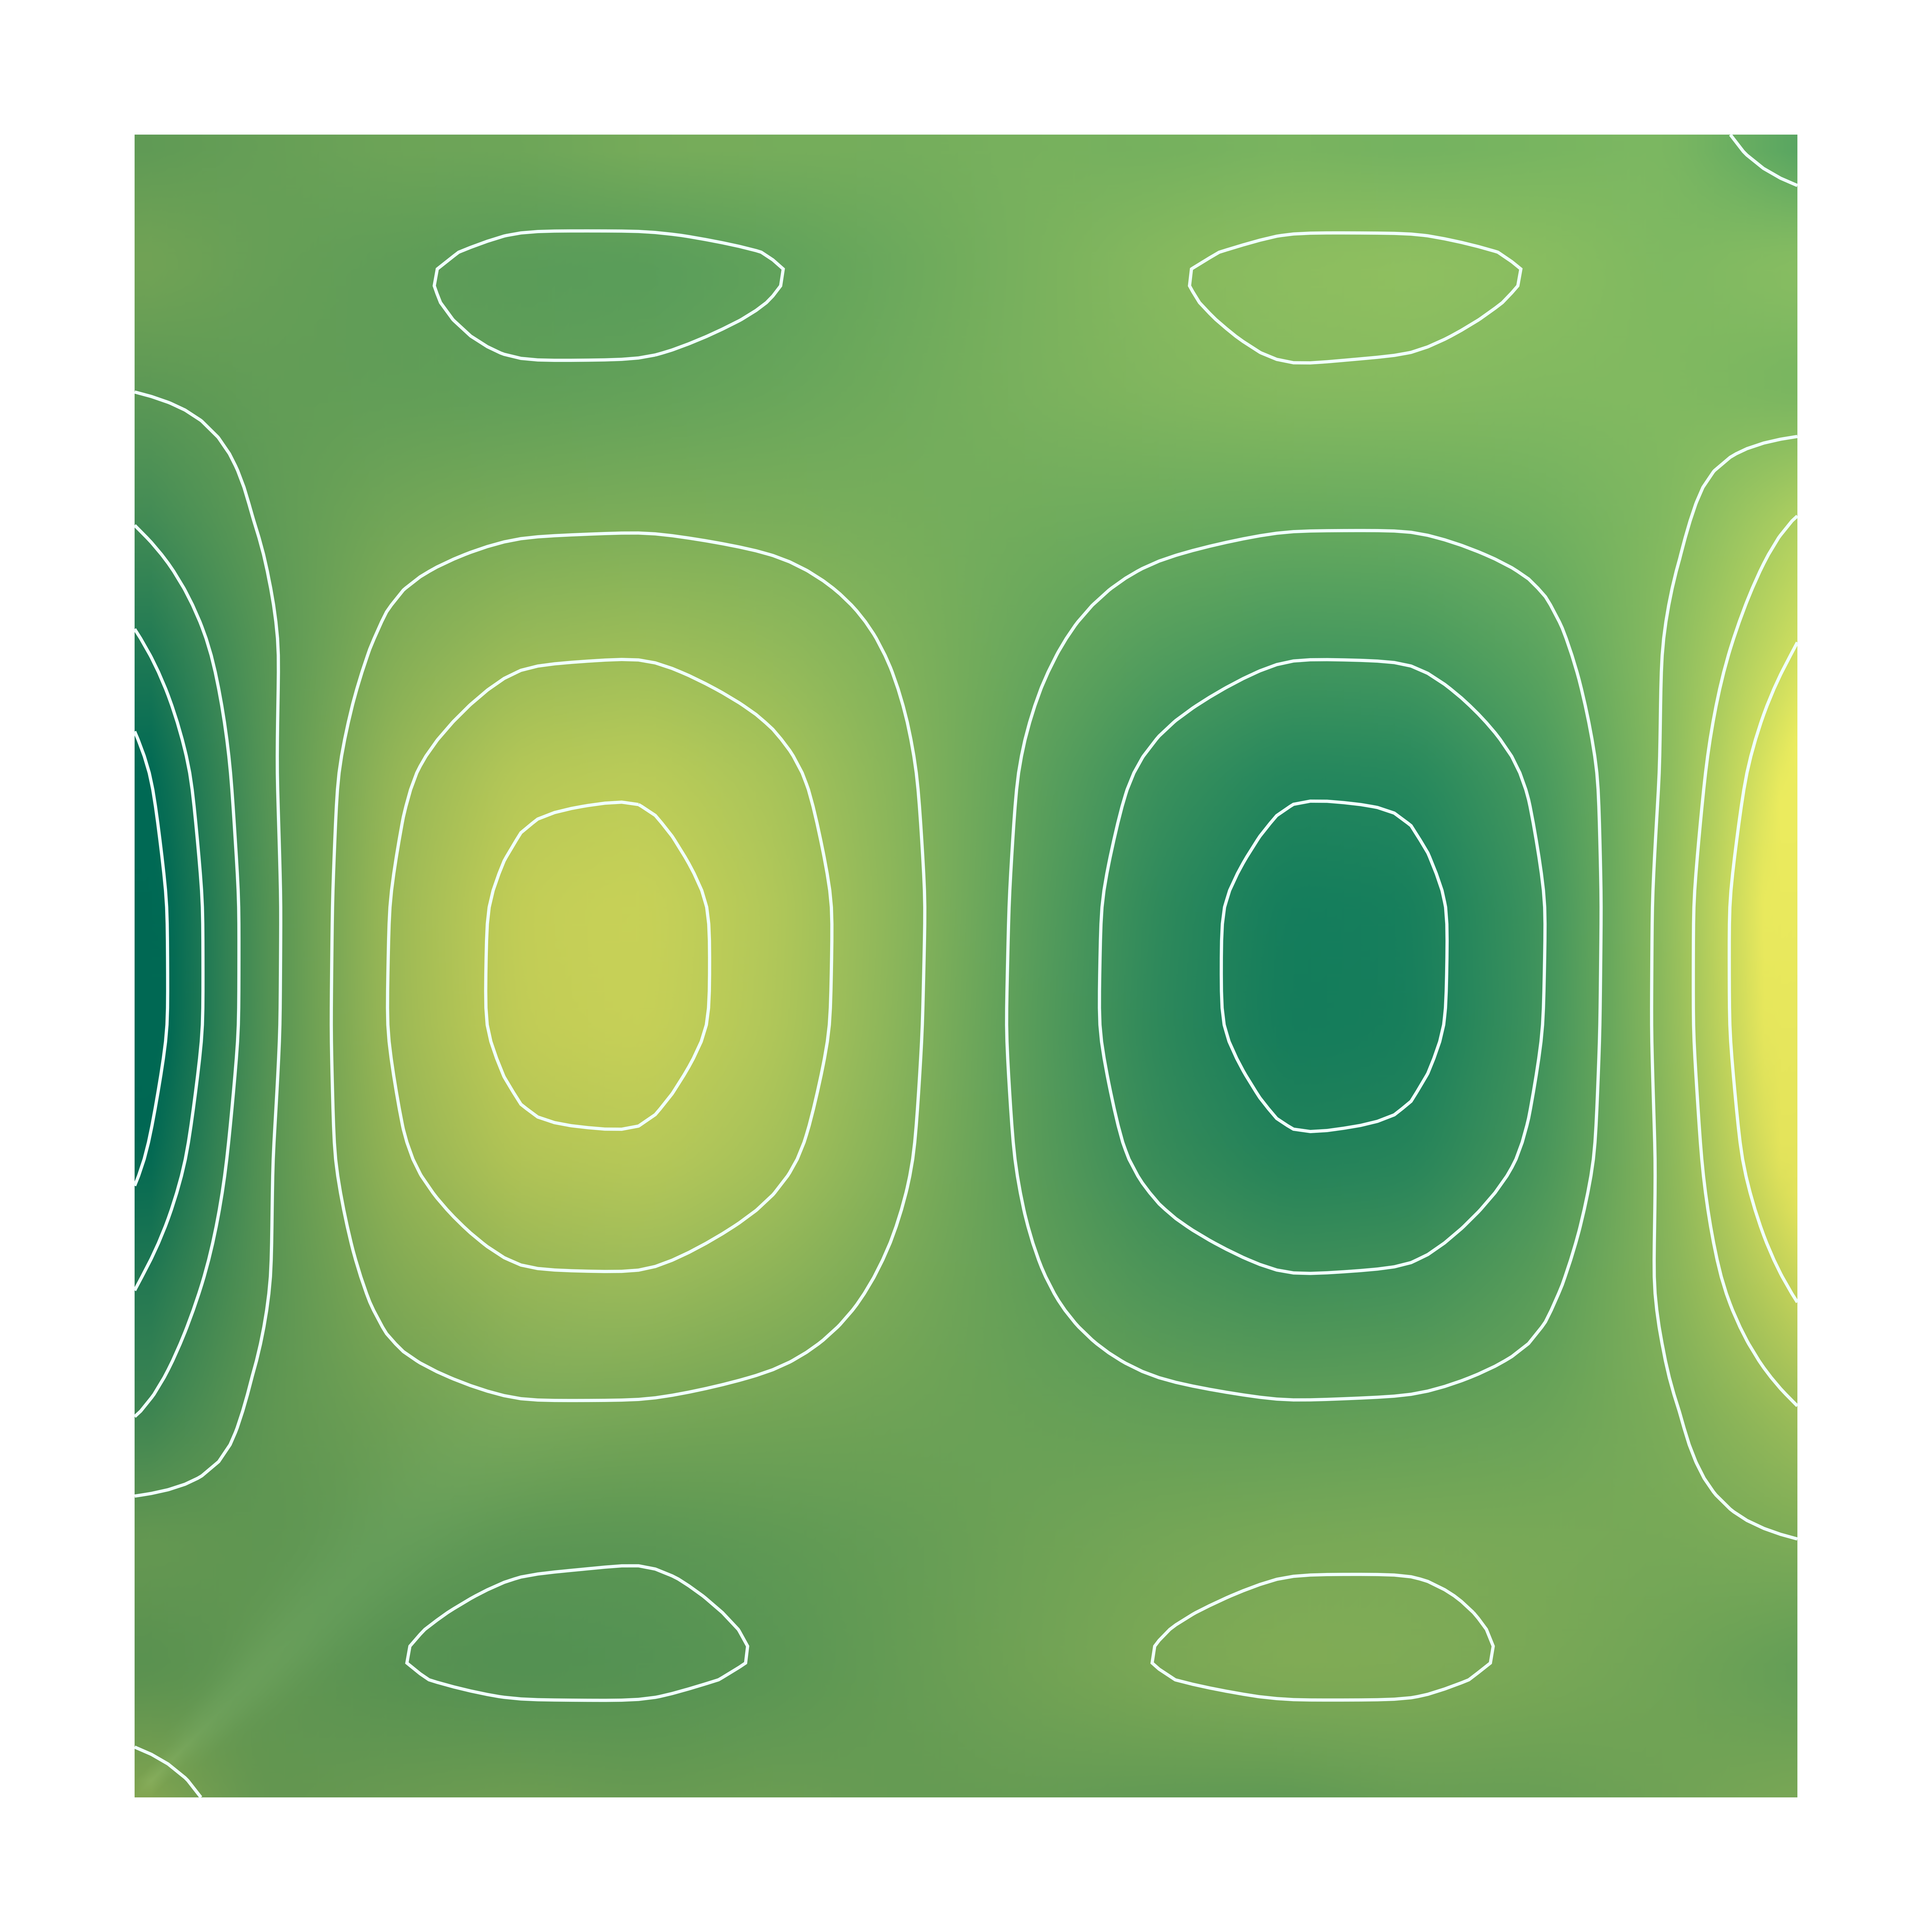
\includegraphics[width=0.4\textwidth]{figures/shearlocking/SquarePlate_mix_quad4_q1_16_13.png}}\end{subcaptiongroup}
    &\begin{subcaptiongroup}\raisebox{-0.5\height}{\includegraphics[width=0.4\textwidth]{figures/shearlocking/SquarePlate_mix_quad4_q1_16_16.png}}\end{subcaptiongroup}\\
    $1089$&\begin{subcaptiongroup}\raisebox{-0.5\height}{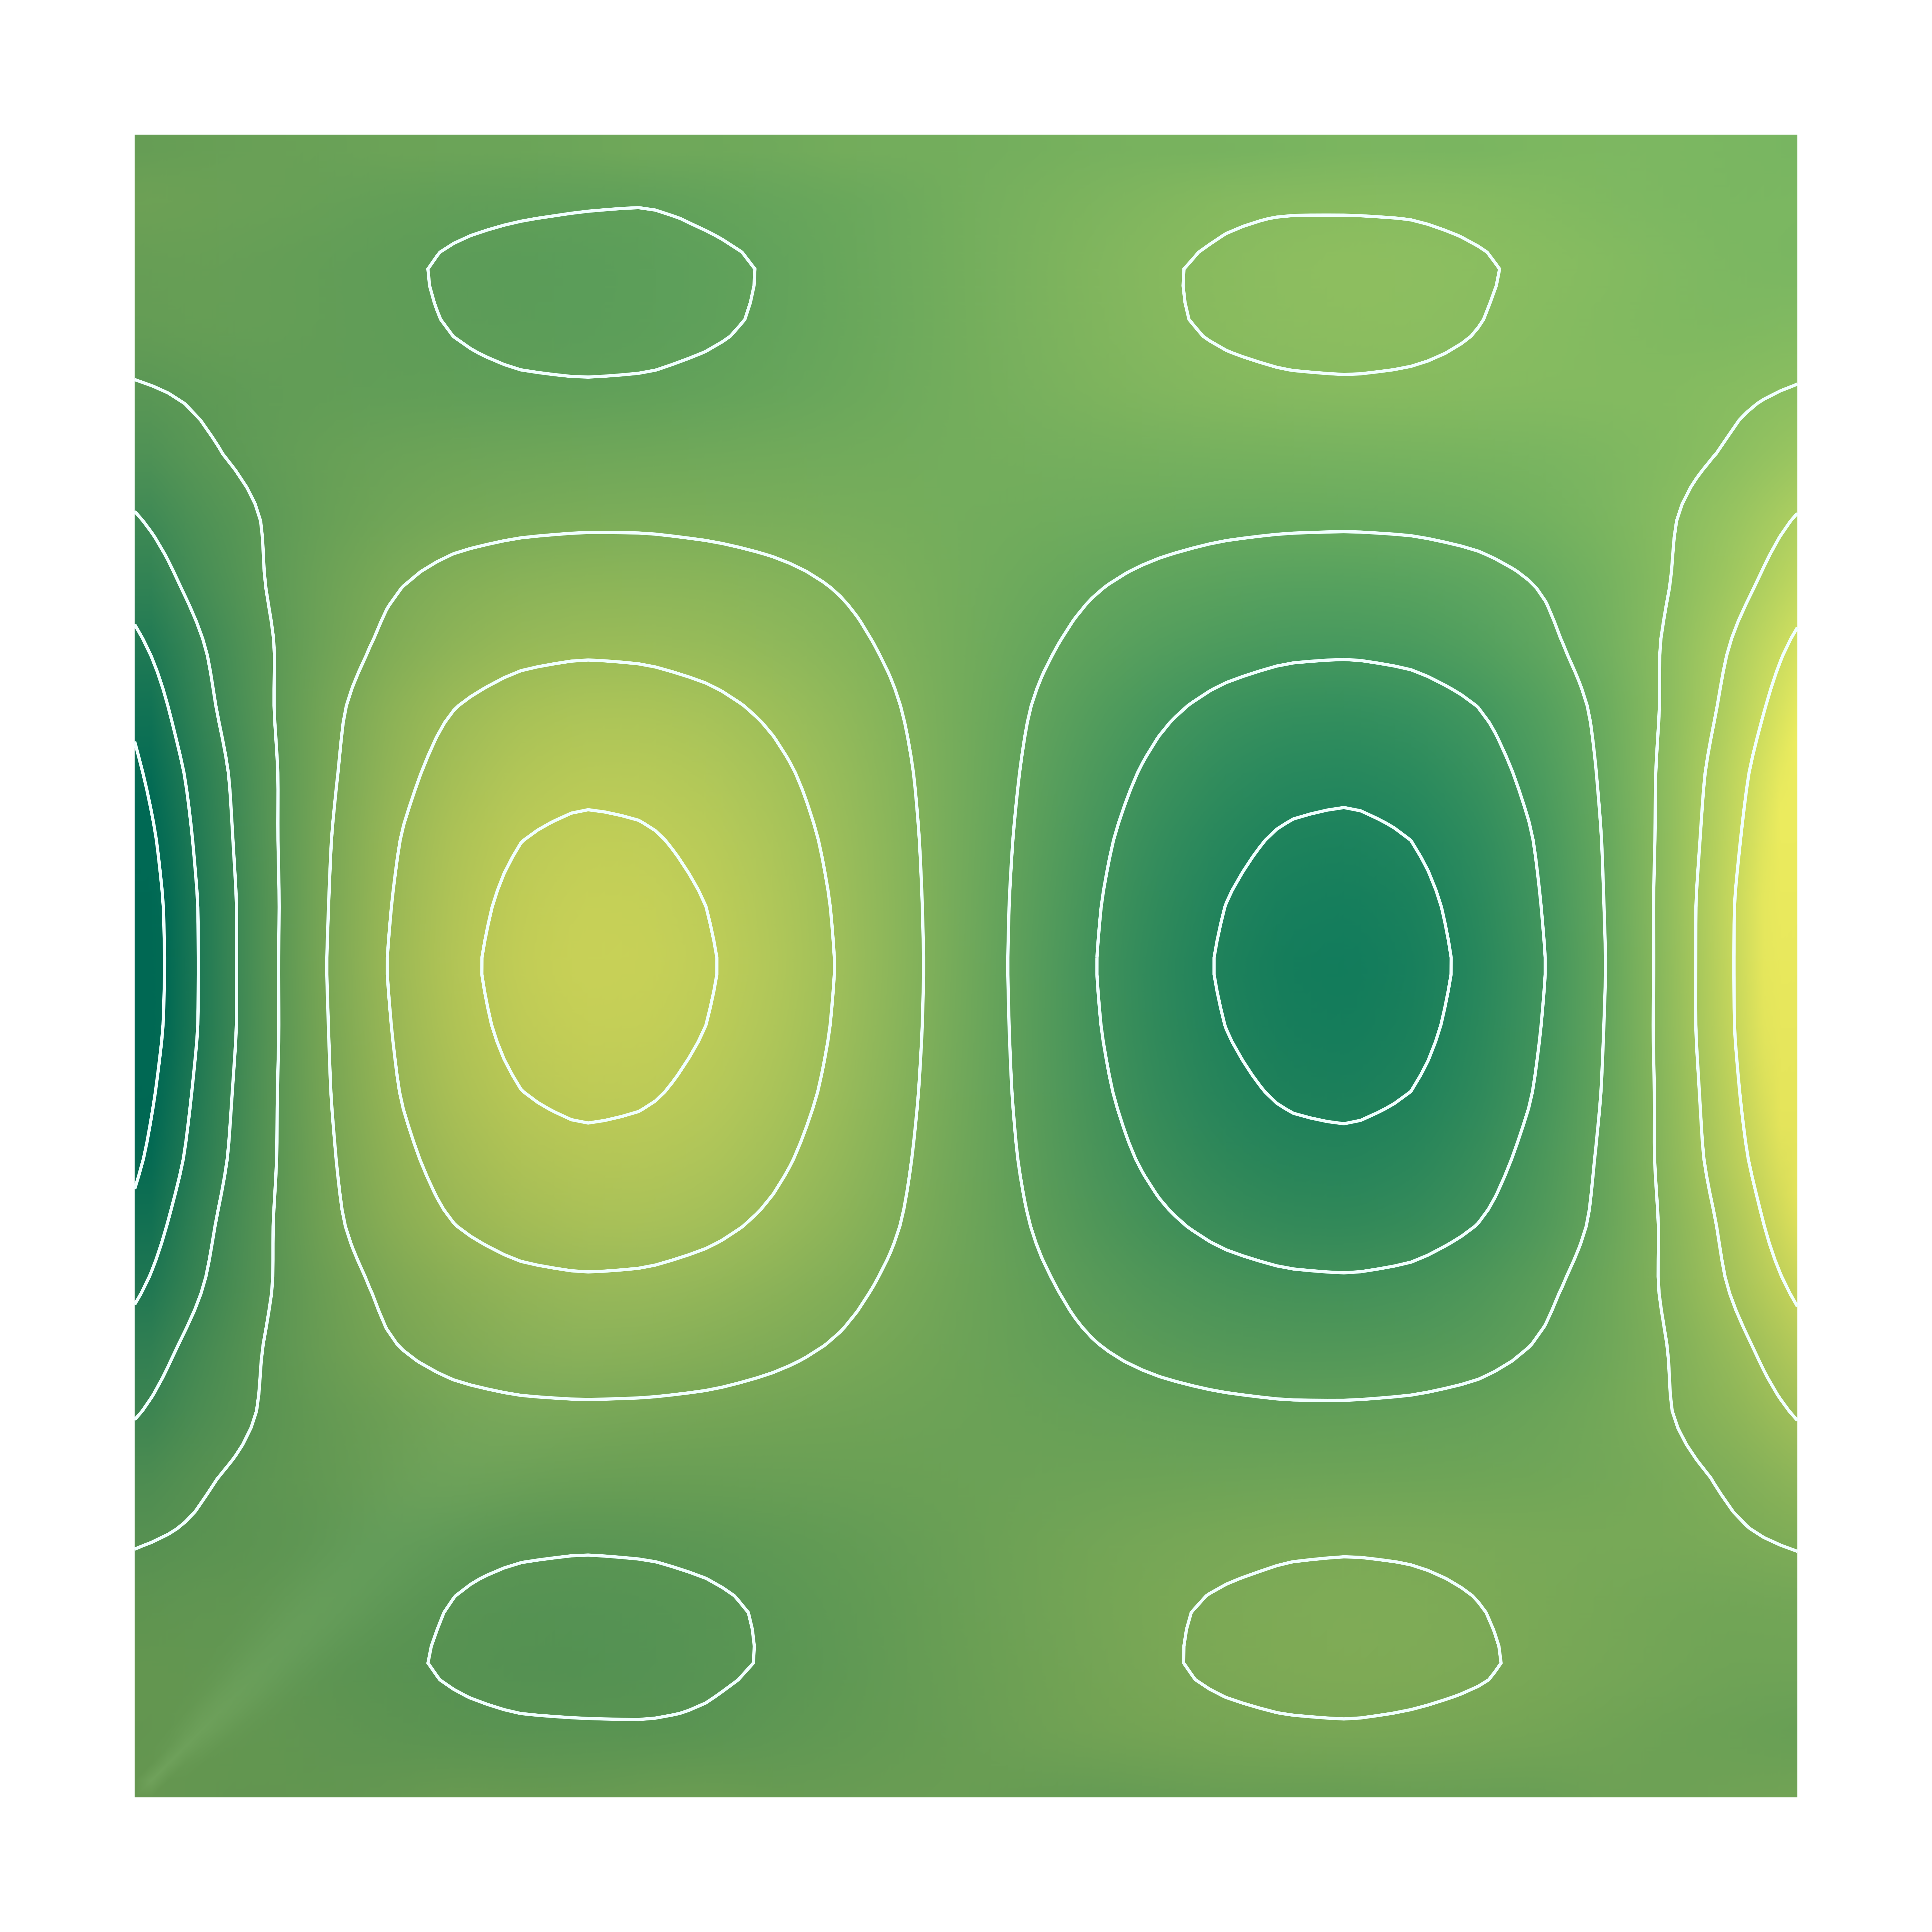
\includegraphics[width=0.4\textwidth]{figures/shearlocking/SquarePlate_mix_quad4_q1_32_26.png}}\end{subcaptiongroup}
    &\begin{subcaptiongroup}\raisebox{-0.5\height}{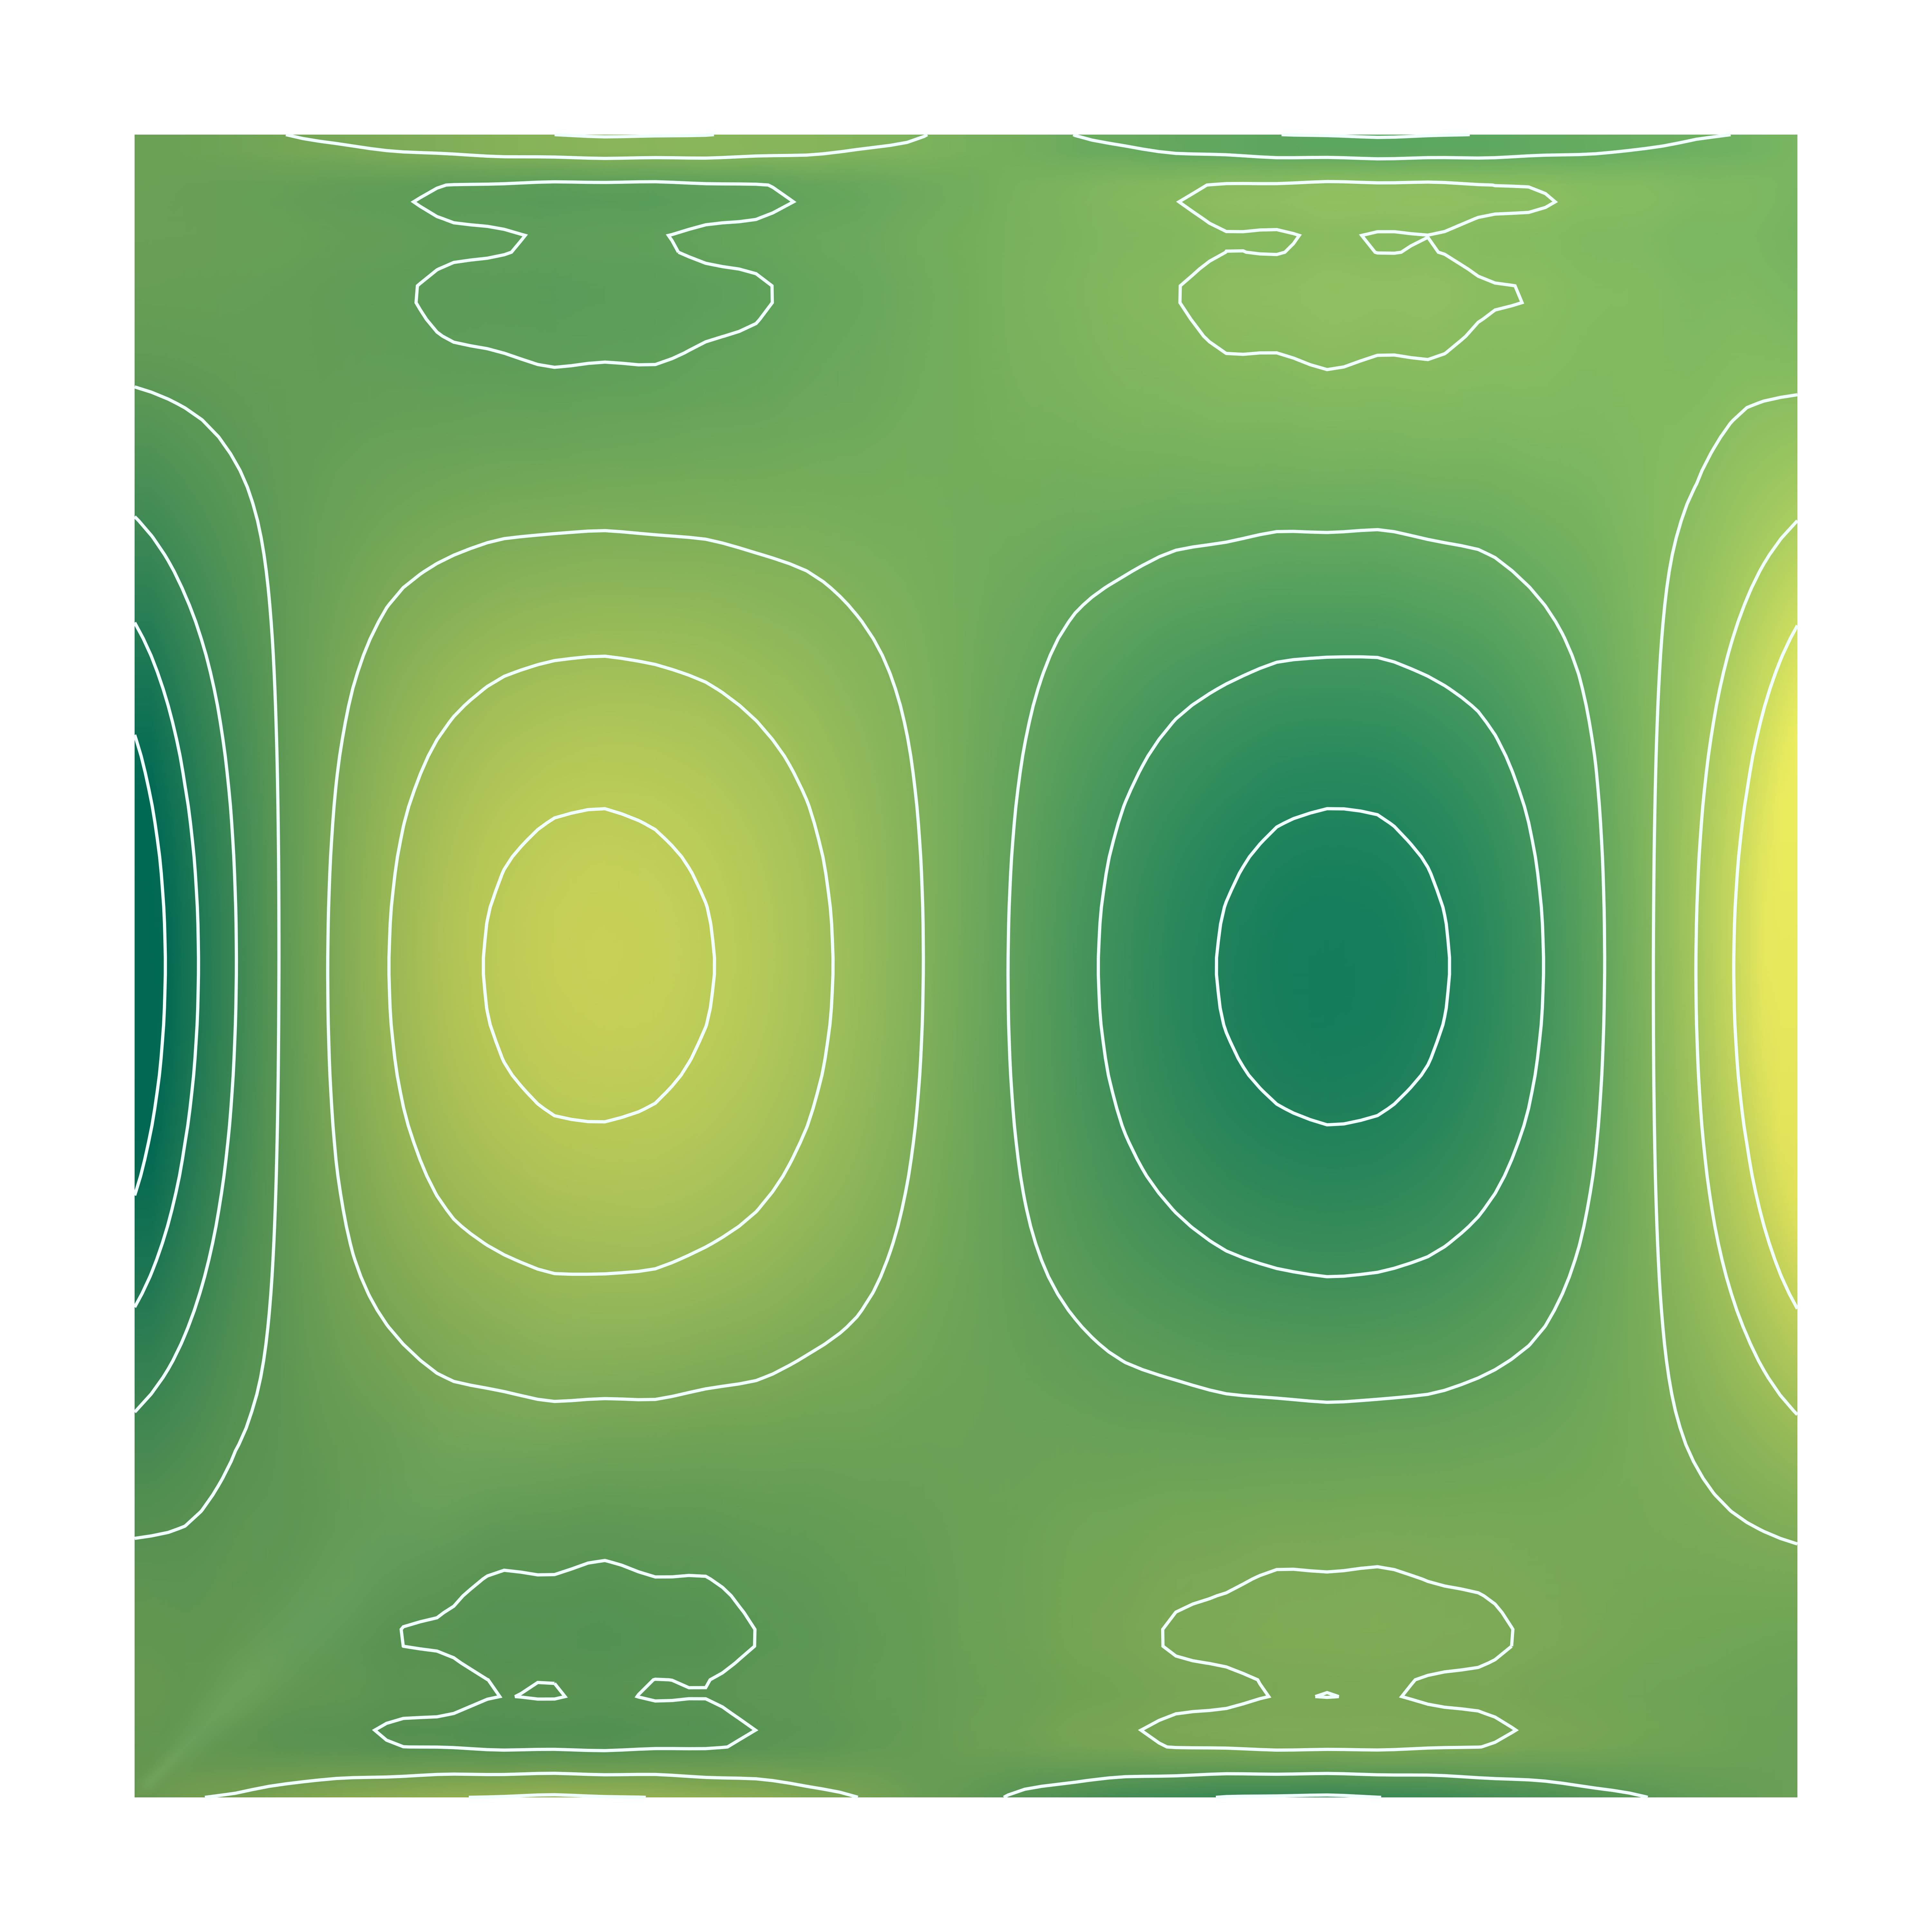
\includegraphics[width=0.4\textwidth]{figures/shearlocking/SquarePlate_mix_quad4_q1_32_32.png}}\end{subcaptiongroup}\\
    \end{tabular}
    \caption{\textbf{固支方板问题Quad4单元应力云图($Q_1$)}}\label{ch_5:fig:Q1_Quad4}
\end{figure}

\begin{figure}[!h]
    \centering
    \begin{tabular}{cccc}
    $\quad$&最优约束比&传统约束比\\
    $289$&\begin{subcaptiongroup}\raisebox{-0.5\height}{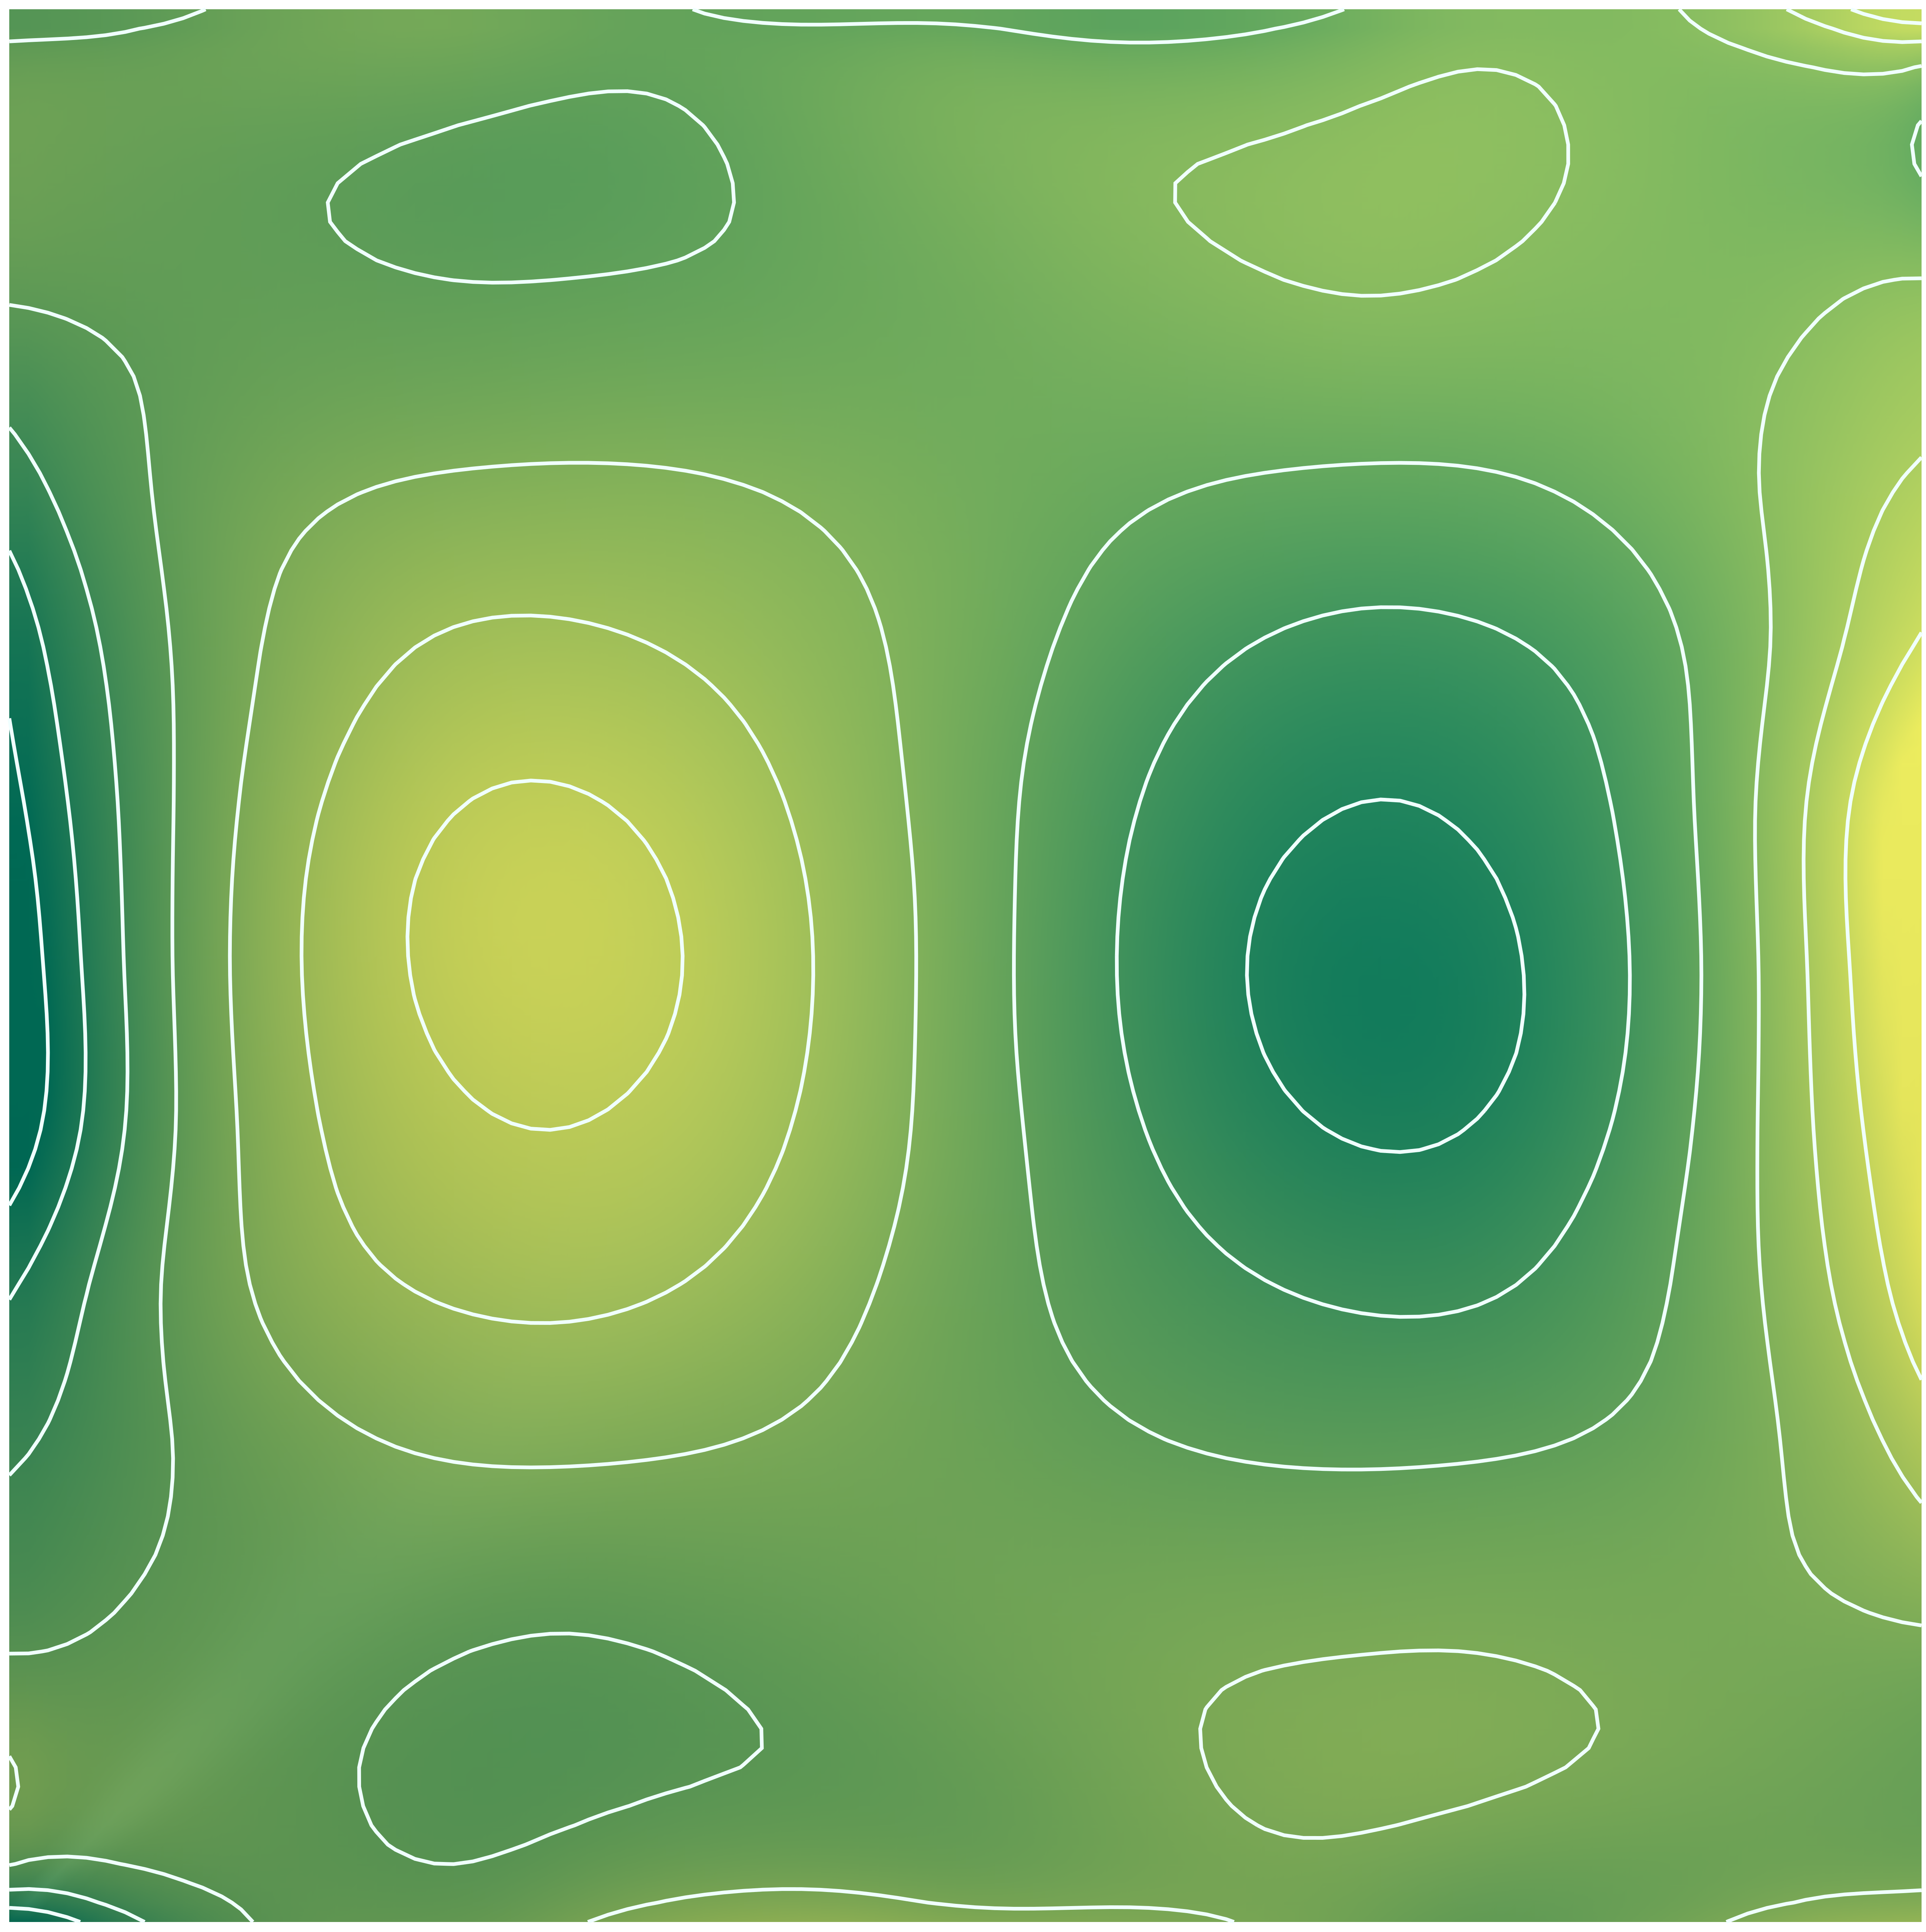
\includegraphics[width=0.4\textwidth]{figures/shearlocking/SquarePlate_mix_tri6_q1_8_6.png}}\end{subcaptiongroup}
    &\begin{subcaptiongroup}\raisebox{-0.5\height}{\includegraphics[width=0.4\textwidth]{figures/shearlocking/SquarePlate_mix_tri6_q1_8_8.png}}\end{subcaptiongroup}\\
    $1089$&\begin{subcaptiongroup}\raisebox{-0.5\height}{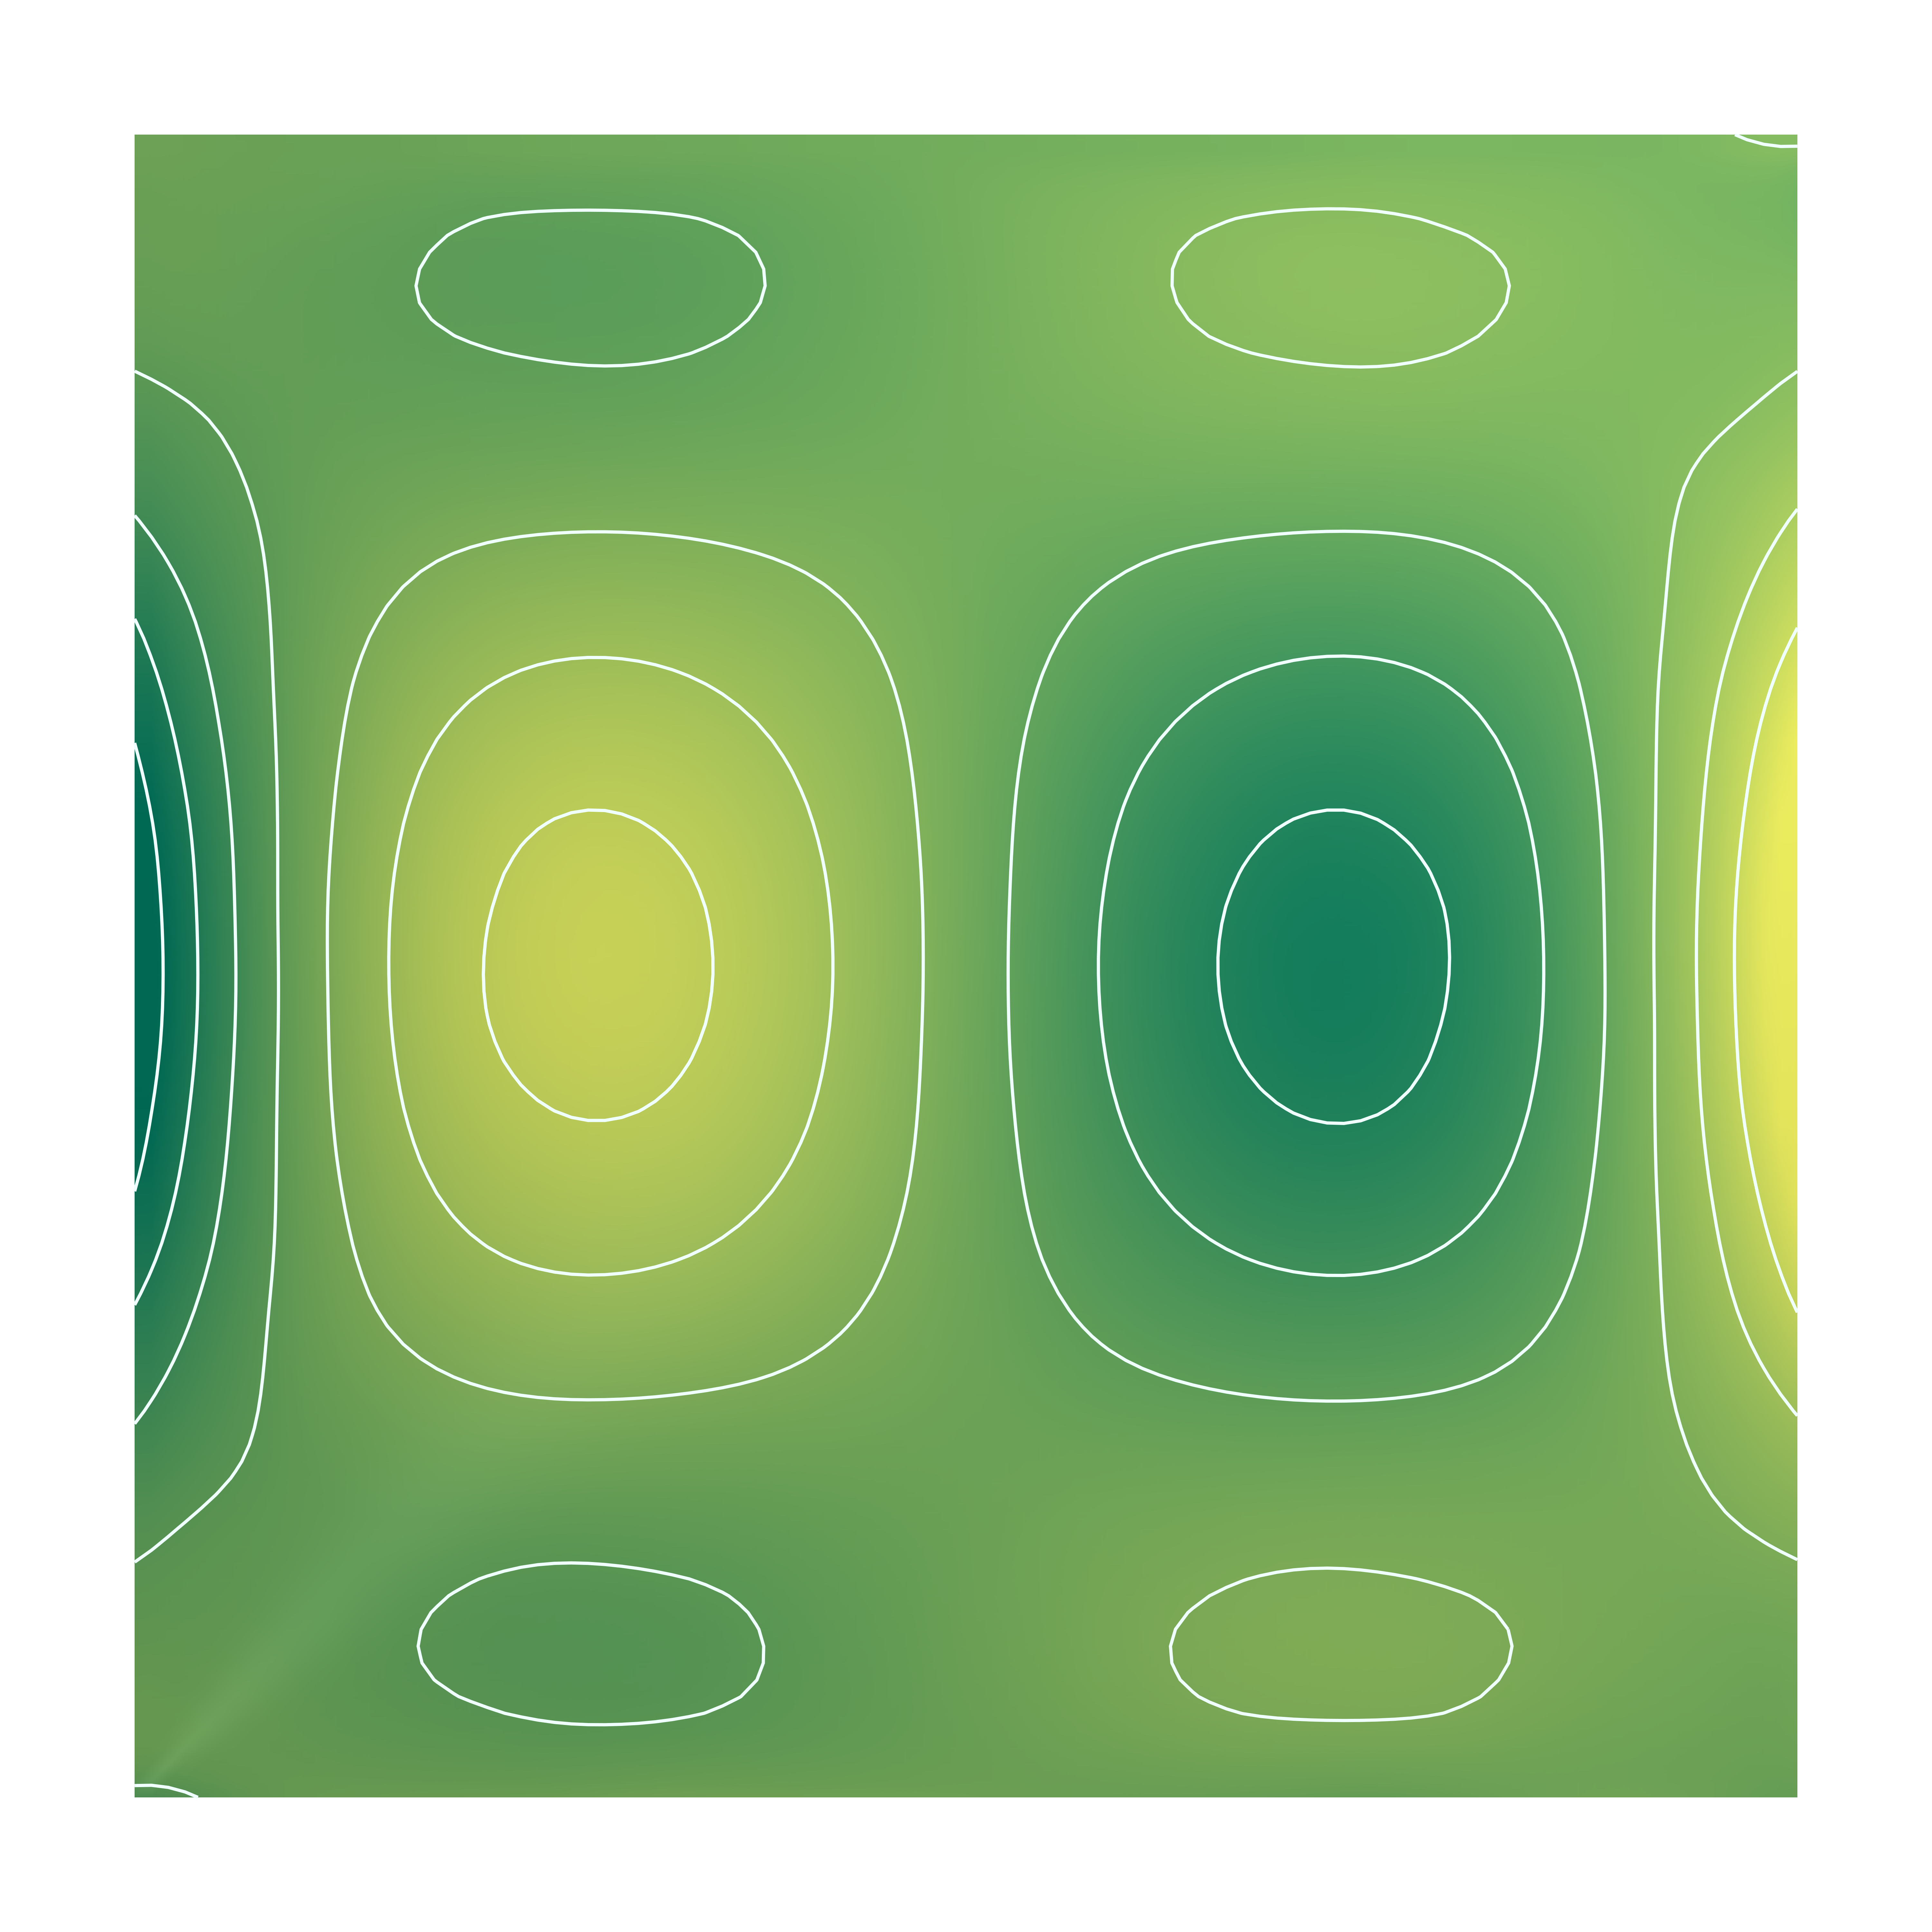
\includegraphics[width=0.4\textwidth]{figures/shearlocking/SquarePlate_mix_tri6_q1_16_12.png}}\end{subcaptiongroup}
    &\begin{subcaptiongroup}\raisebox{-0.5\height}{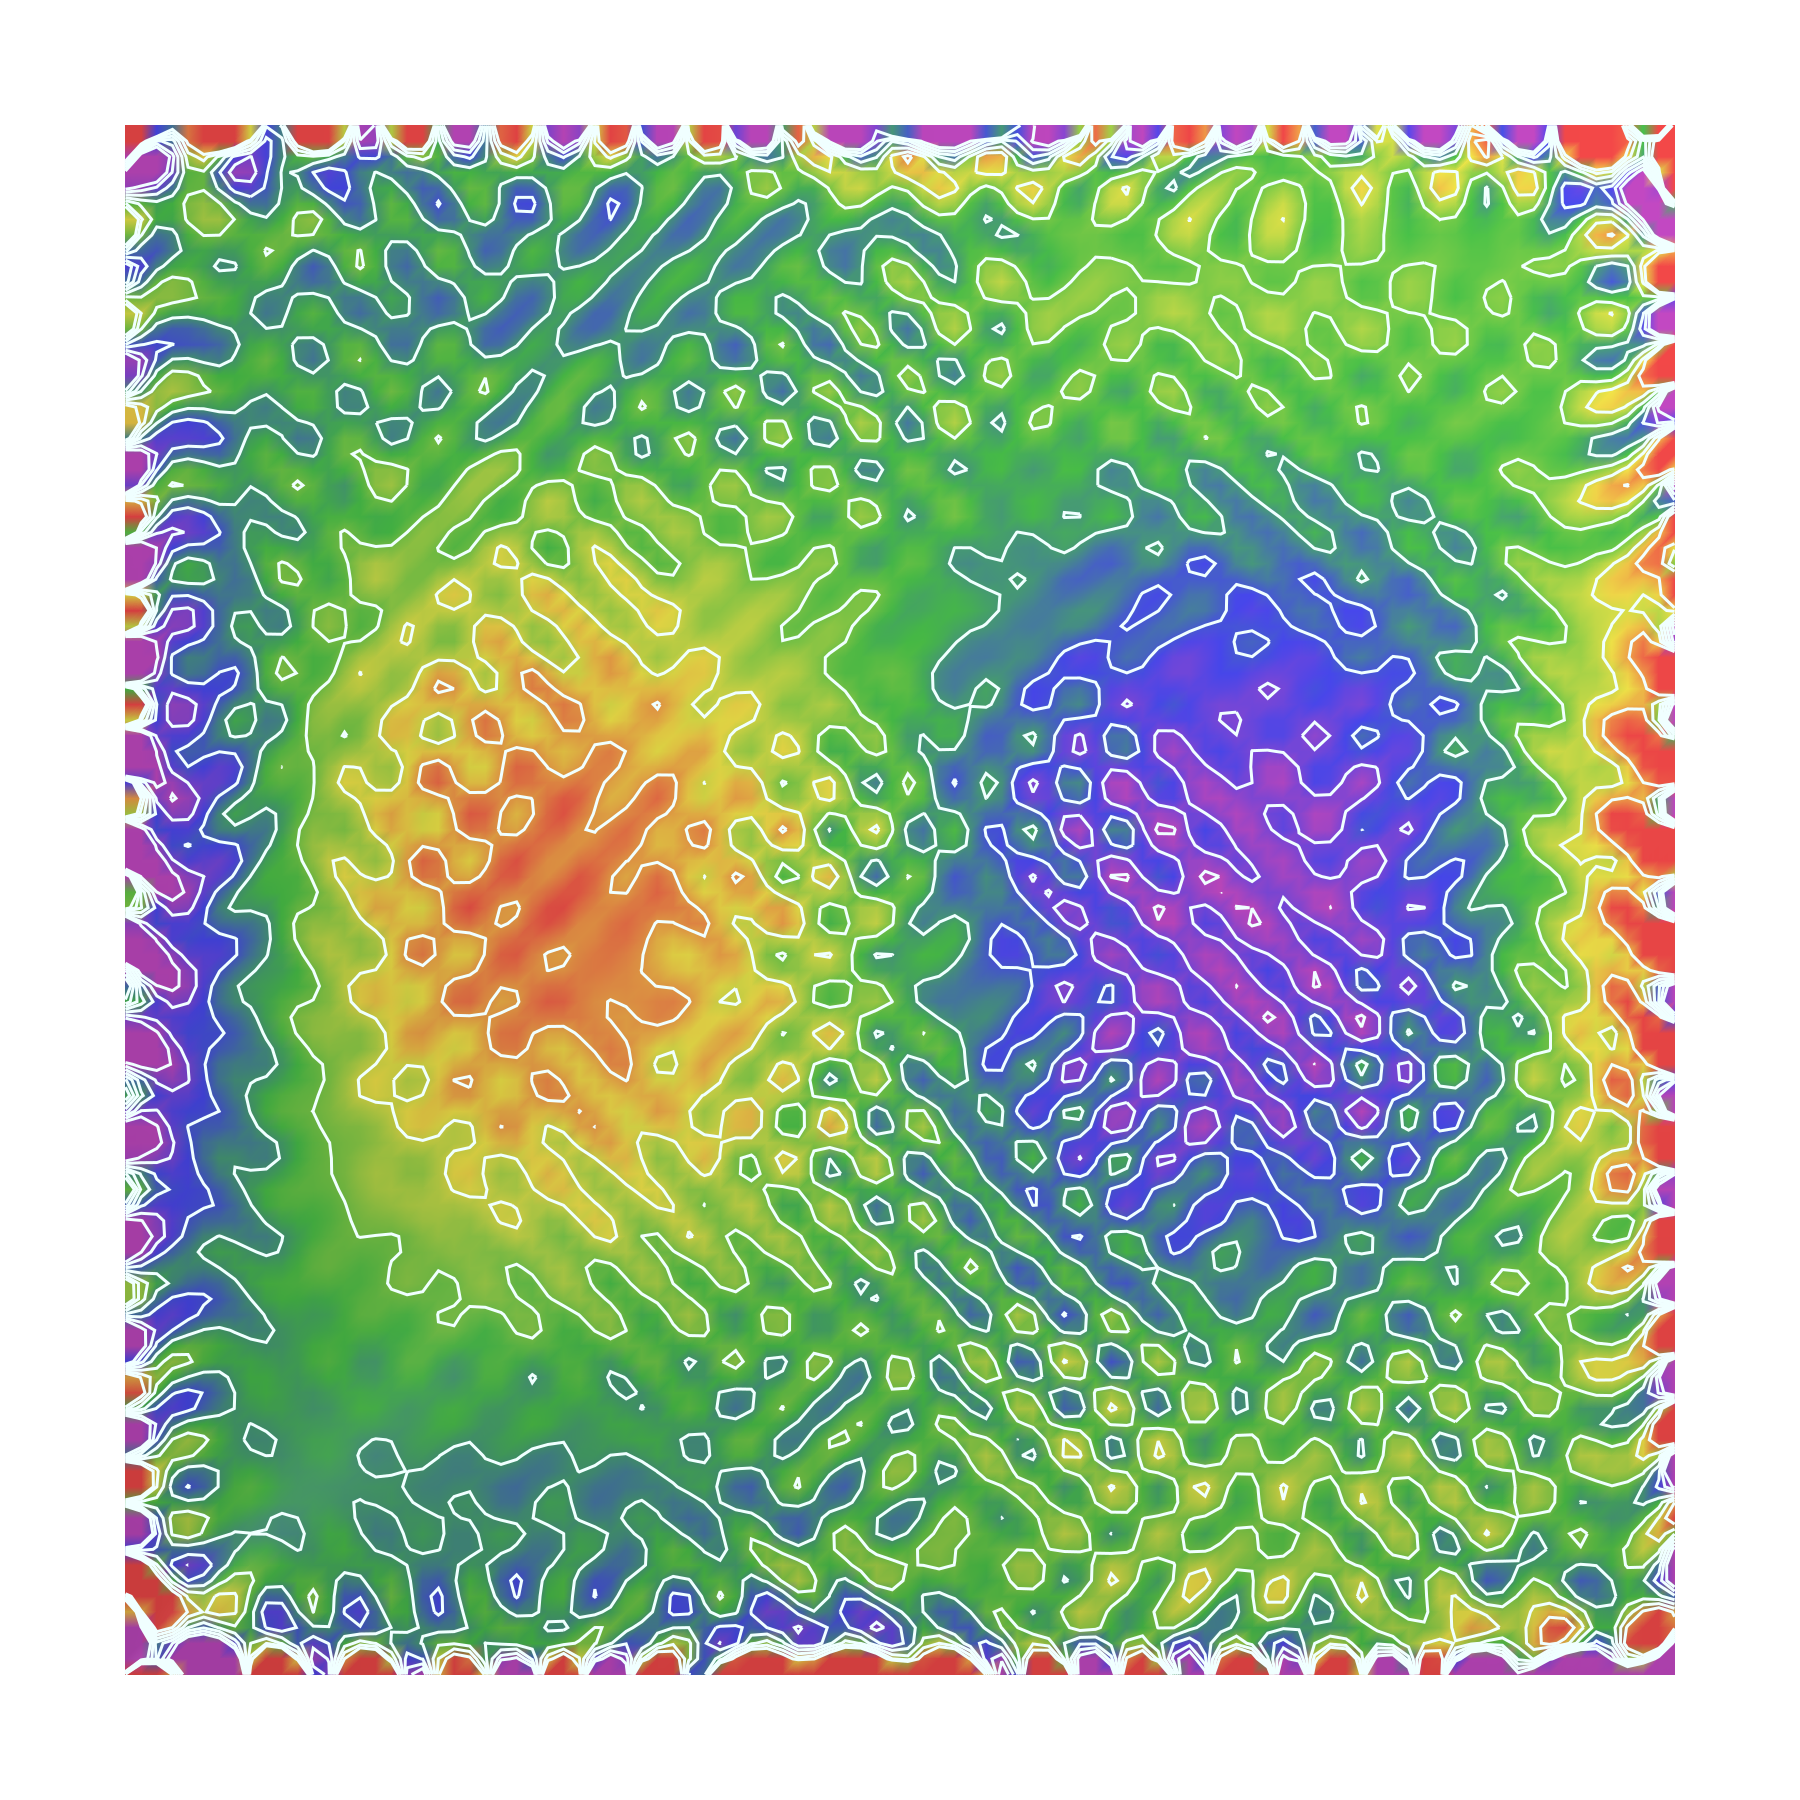
\includegraphics[width=0.4\textwidth]{figures/shearlocking/SquarePlate_mix_tri6_q1_16_16.png}}\end{subcaptiongroup}\\
    $4225$&\begin{subcaptiongroup}\raisebox{-0.5\height}{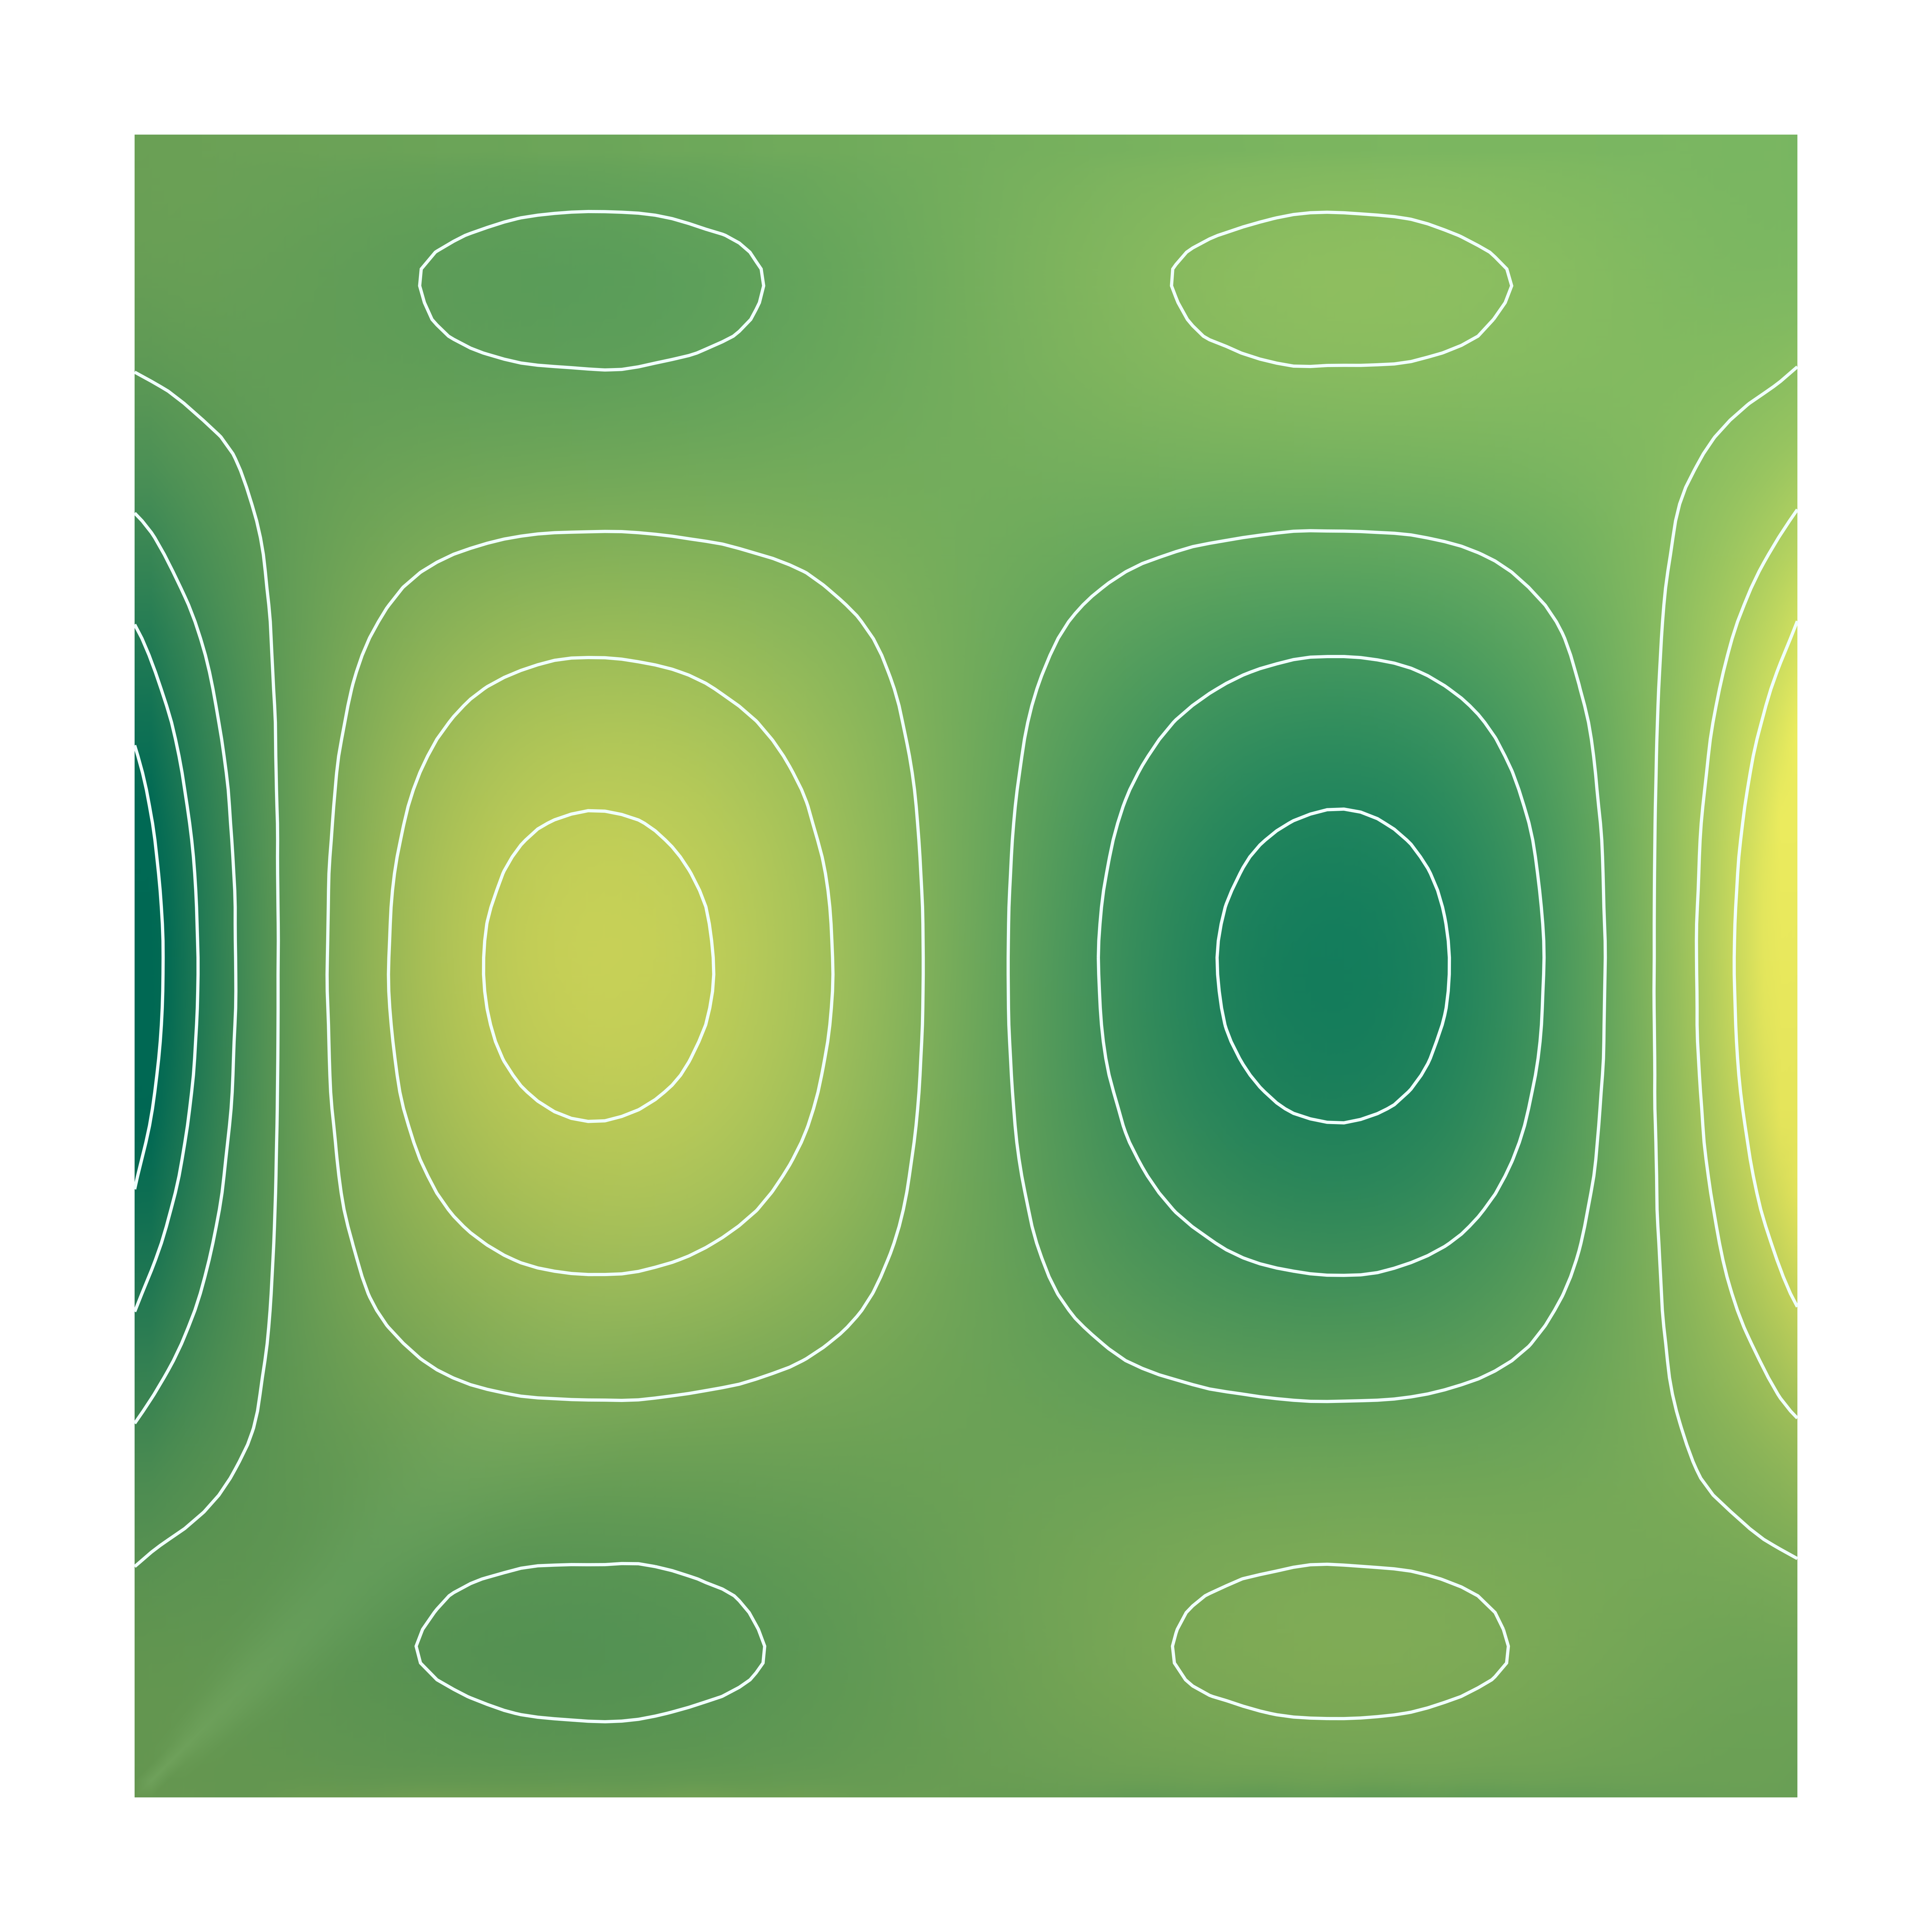
\includegraphics[width=0.4\textwidth]{figures/shearlocking/SquarePlate_mix_tri6_q1_32_25.png}}\end{subcaptiongroup}
    &\begin{subcaptiongroup}\raisebox{-0.5\height}{\includegraphics[width=0.4\textwidth]{figures/shearlocking/SquarePlate_mix_tri6_q1_32_32.png}}\end{subcaptiongroup}\\  
    \end{tabular}
    \caption{\textbf{固支方板问题Tri6单元应力云图($Q_1$)}}\label{ch_5:fig:Q1_Tri6}
\end{figure}

\begin{figure}[!h]
    \centering
    \begin{tabular}{cccc}
    $\quad$&最优约束比&传统约束比\\
    $225$&\begin{subcaptiongroup}\raisebox{-0.4\height}{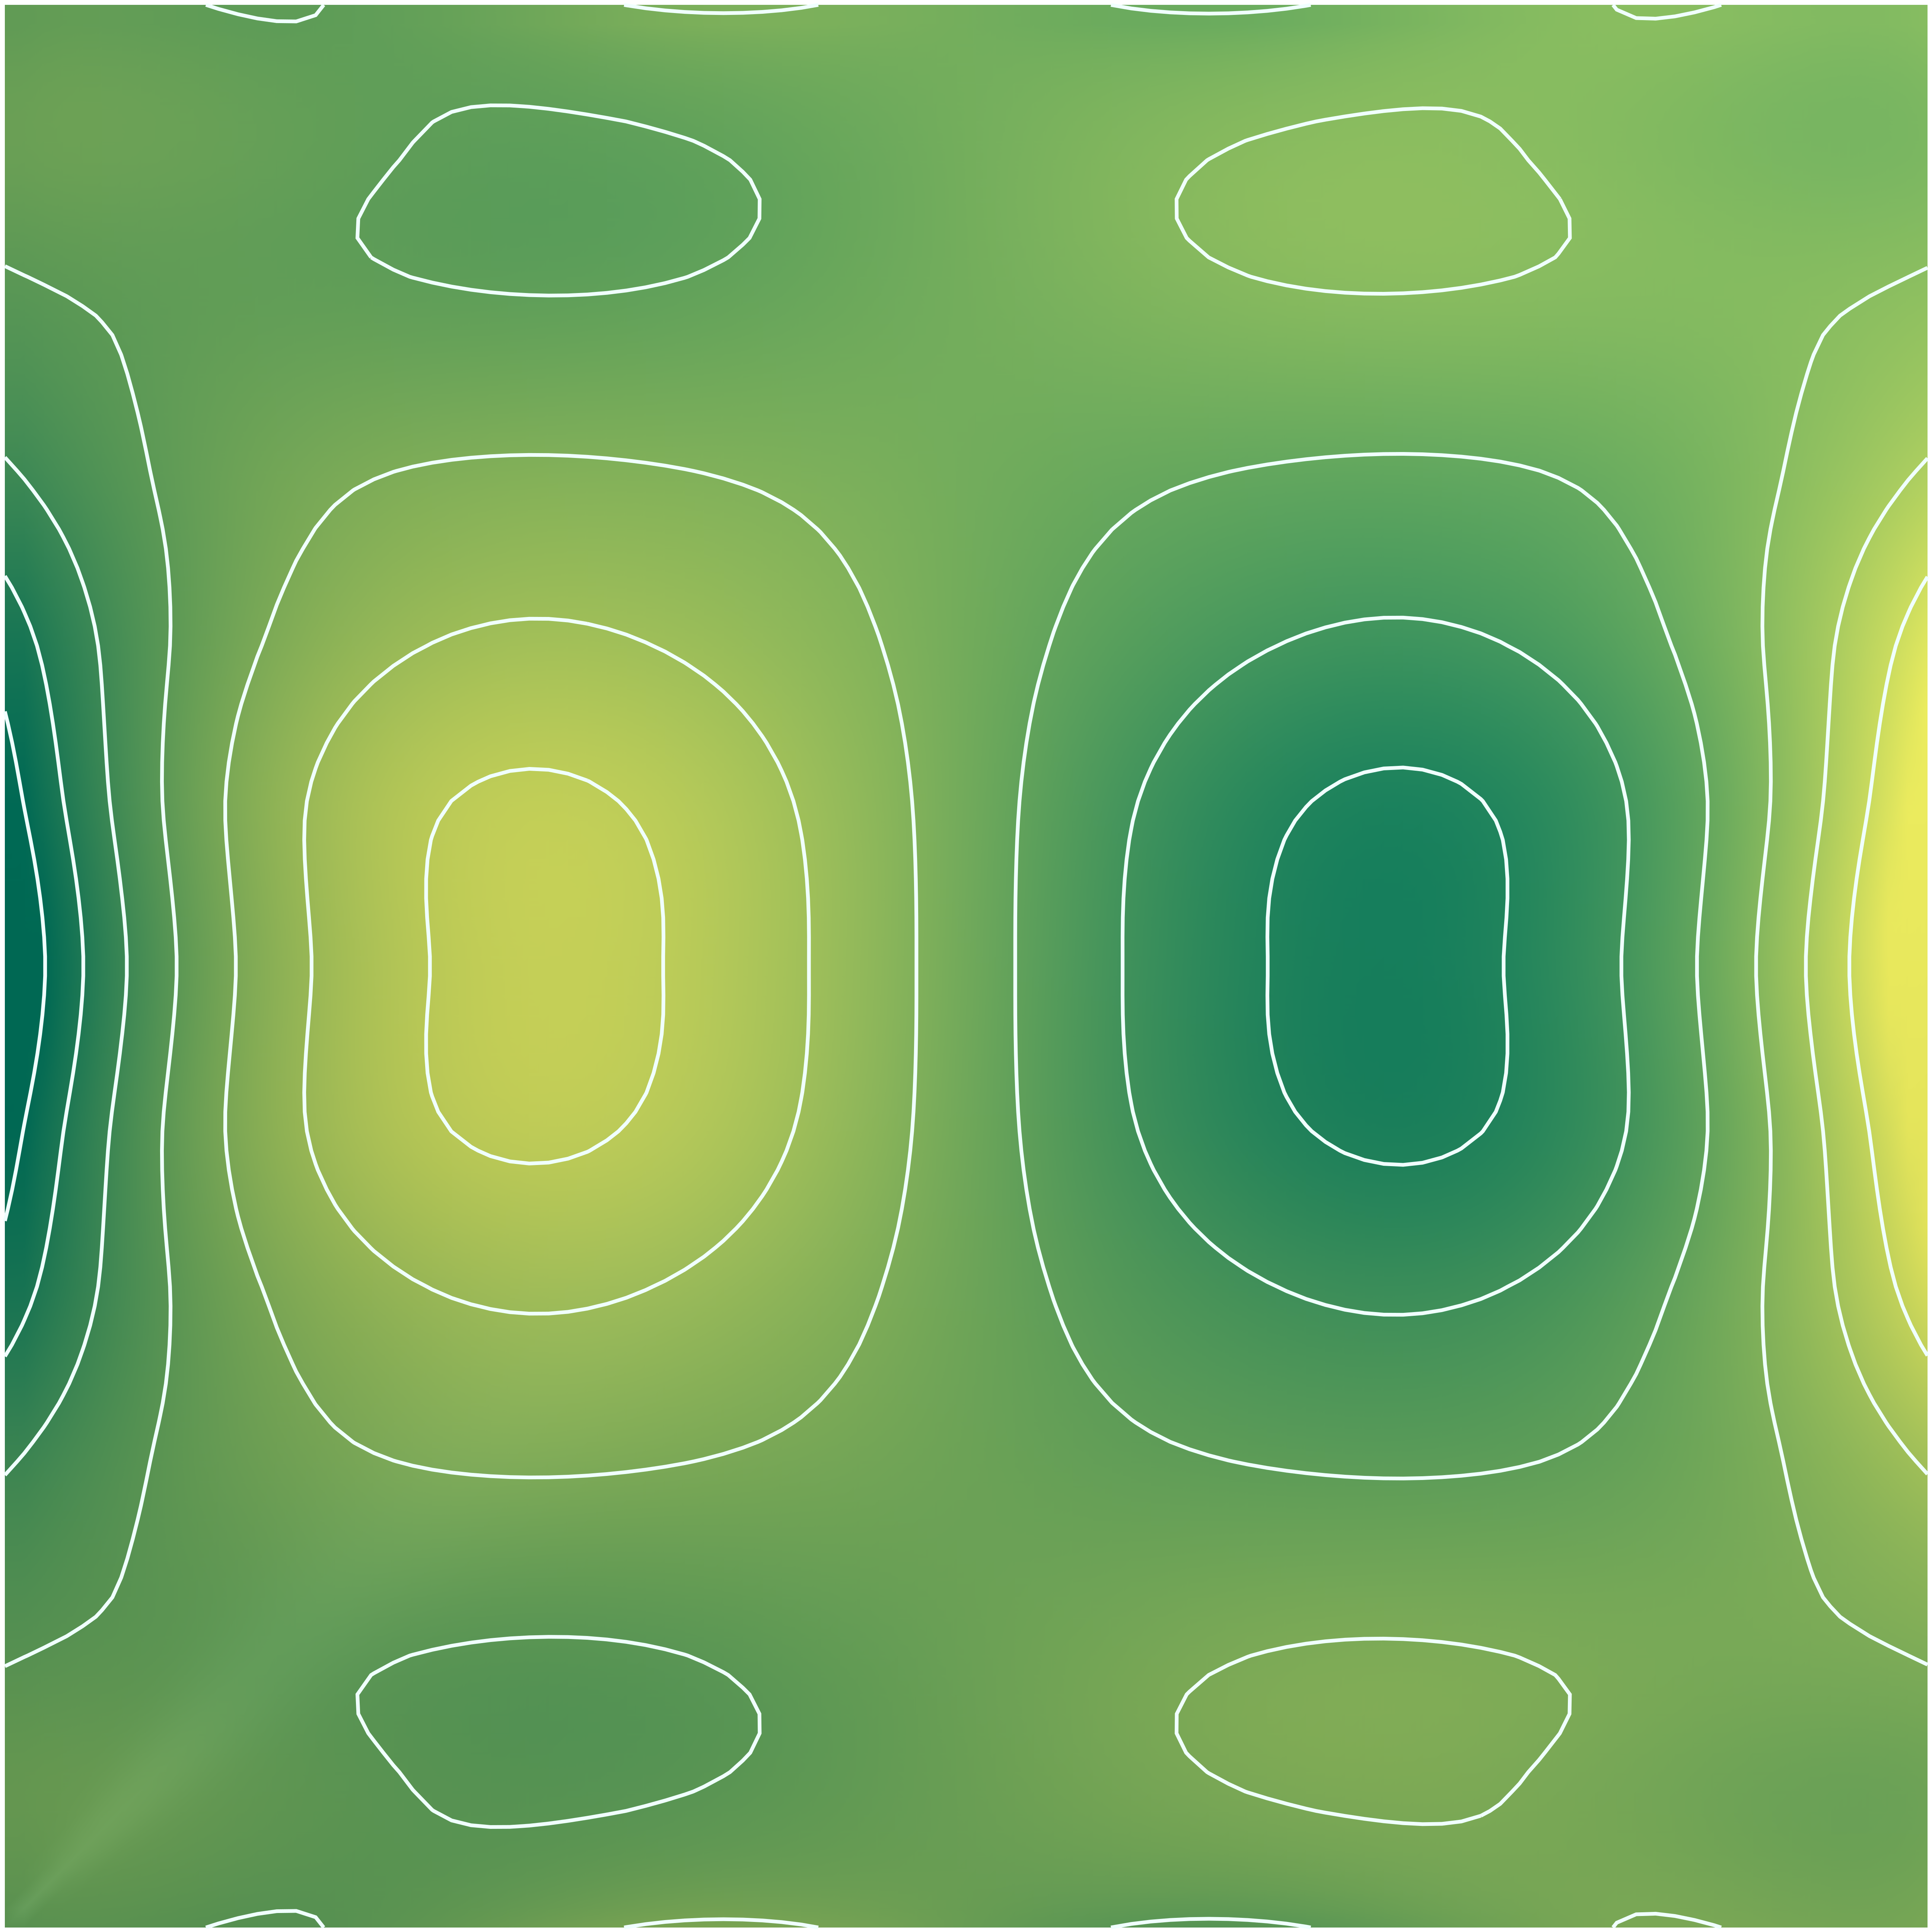
\includegraphics[width=0.4\textwidth]{figures/shearlocking/SquarePlate_mix_quad8_q1_8_6.png}}\end{subcaptiongroup}
    &\begin{subcaptiongroup}\raisebox{-0.4\height}{\includegraphics[width=0.4\textwidth]{figures/shearlocking/SquarePlate_mix_quad8_q1_8_8.png}}\end{subcaptiongroup}\\
    $833$&\begin{subcaptiongroup}\raisebox{-0.4\height}{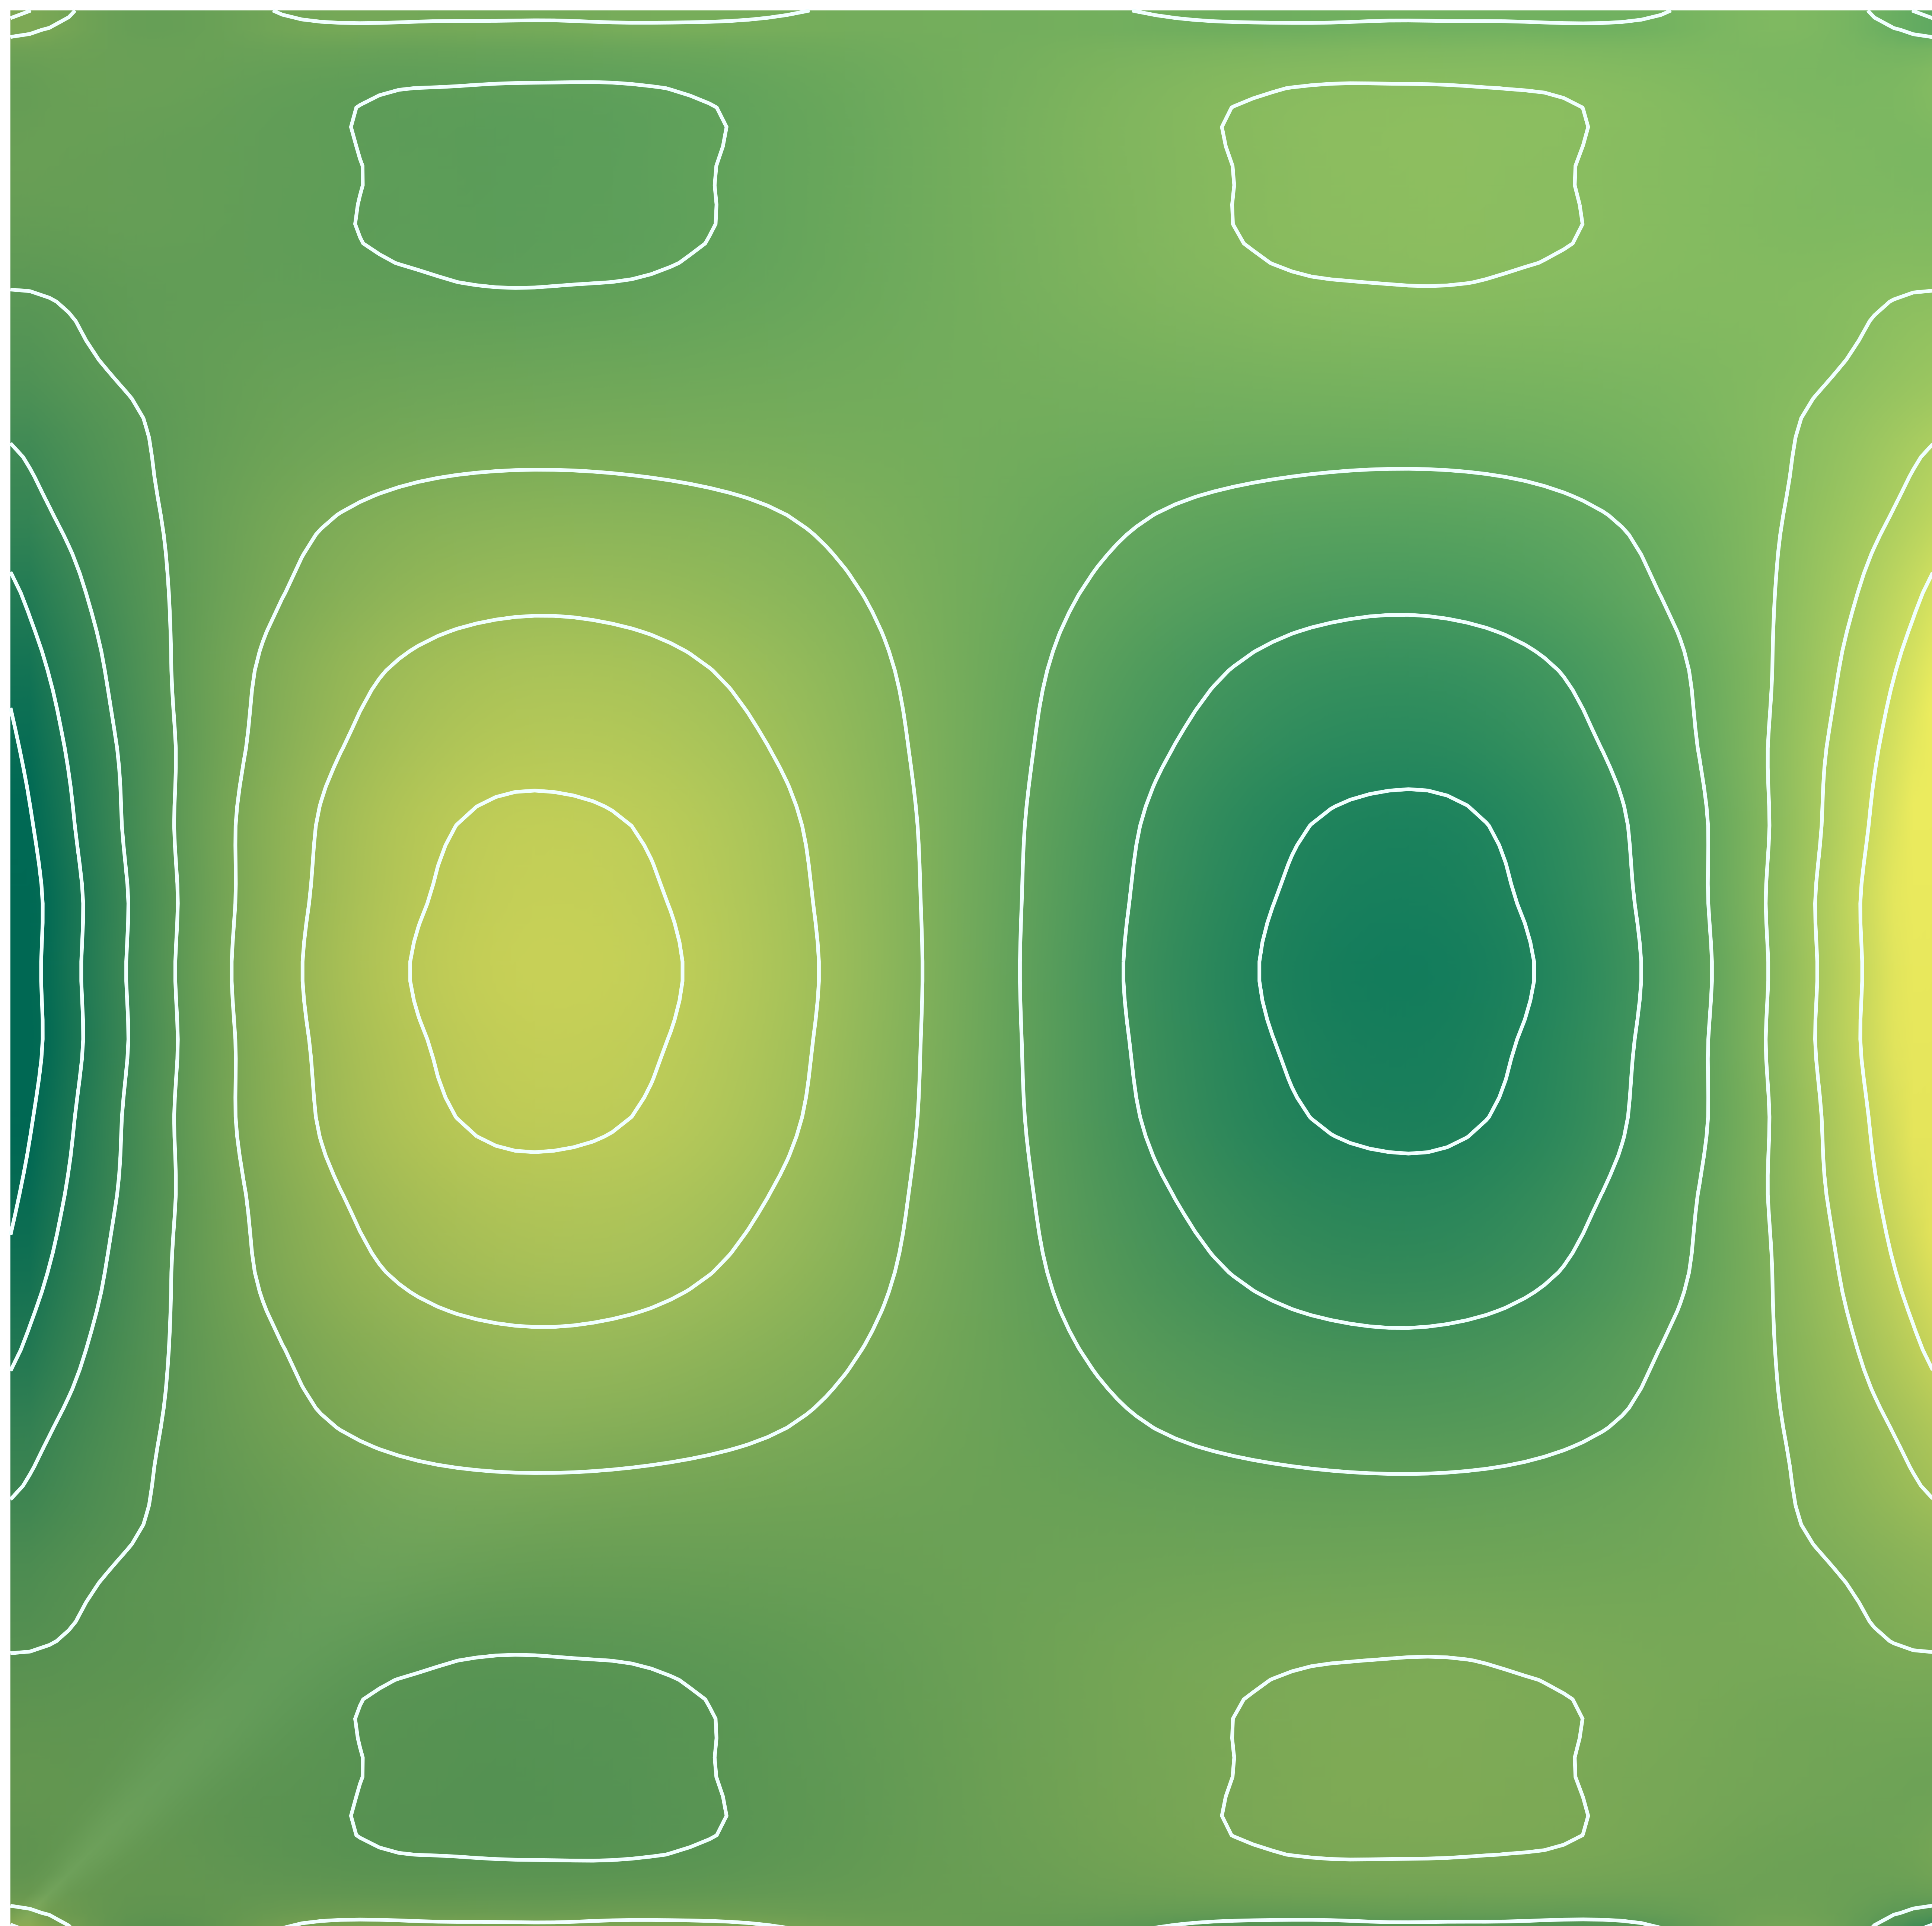
\includegraphics[width=0.4\textwidth]{figures/shearlocking/SquarePlate_mix_quad8_q1_16_14.png}}\end{subcaptiongroup}
    &\begin{subcaptiongroup}\raisebox{-0.4\height}{\includegraphics[width=0.4\textwidth]{figures/shearlocking/SquarePlate_mix_quad8_q1_16_16.png}}\end{subcaptiongroup}\\
    $3201$&\begin{subcaptiongroup}\raisebox{-0.4\height}{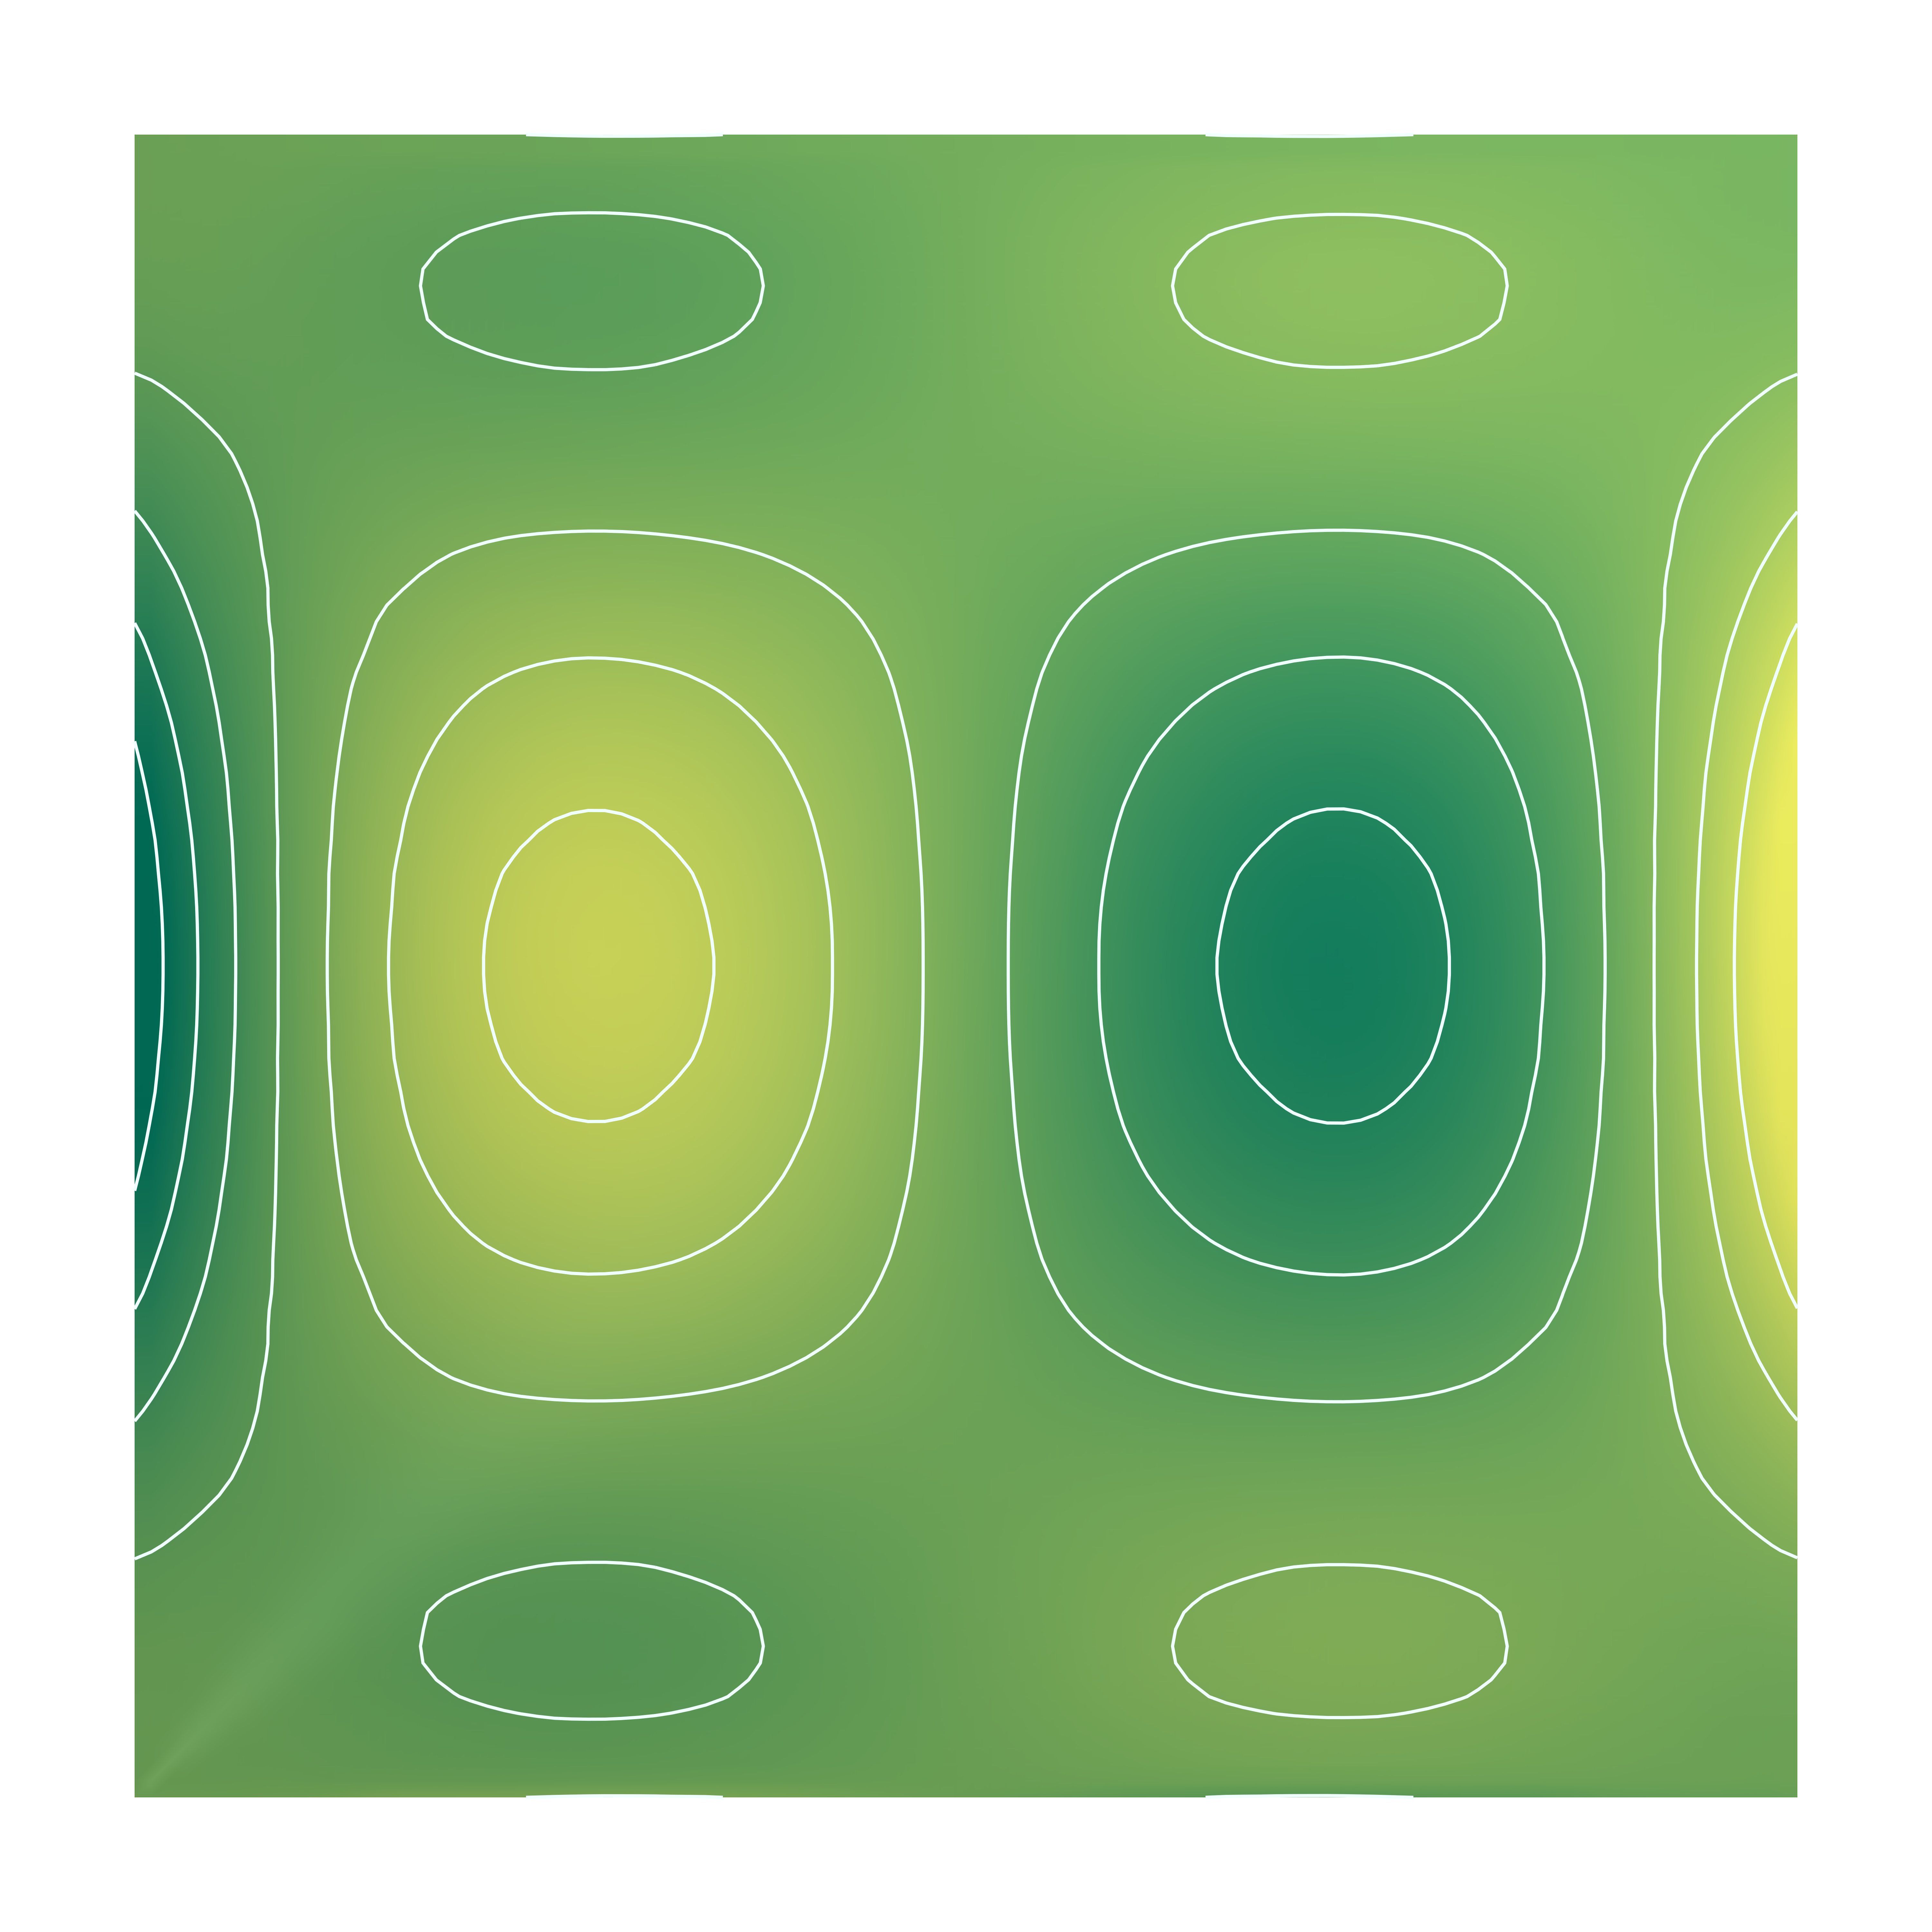
\includegraphics[width=0.4\textwidth]{figures/shearlocking/SquarePlate_mix_quad8_q1_32_26.png}}\end{subcaptiongroup}
    &\begin{subcaptiongroup}\raisebox{-0.4\height}{\includegraphics[width=0.4\textwidth]{figures/shearlocking/SquarePlate_mix_quad8_q1_32_32.png}}\end{subcaptiongroup}\\ 
    \end{tabular}
    \caption{\textbf{固支方板问题Quad8单元应力云图($Q_1$)}}\label{ch_5:fig:Q1_Quad8}
\end{figure}

 \subsection{Razzaque斜板问题}
考虑如图\ref{ch_5:fig:xieplate}所示斜板问题,其中斜板的边长为$L=100$,厚度为$h$,均布荷载作用在板内为$\bar{q}=1$,材料系数分别为杨氏模量$E=1085$、泊松比$\nu=0.31$。该斜板中心A点位移$\bar w_A$的参考解为:
\begin{equation} 
    \bar{w_A}=w_c\times10^2\frac{D}{\bar{q}L^4}
\end{equation}
如图\ref{ch_5:fig:xieplatemsh}所示,斜板求解域采用均布离散的81、289、1089、4225四个疏密不同的节点进行离散,同样采用线性单元和二次单元进行数值分析。
\begin{figure}[!h]
    \centering 
        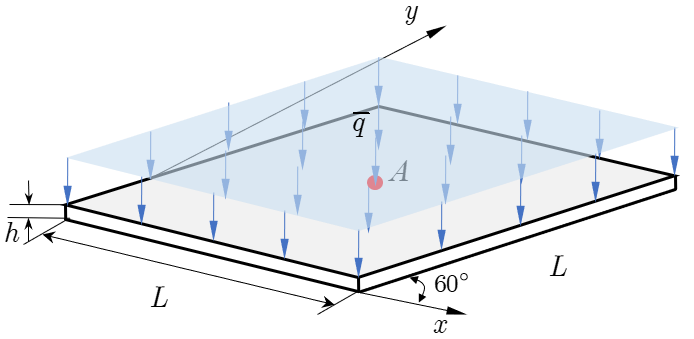
\includegraphics[scale=0.6]{figures/shearlocking/xie plate.png}
        \caption{Razzaque斜板问题模型}\label{ch_5:fig:xieplate}
\end{figure}
\begin{figure}[!h]
    \centering 
        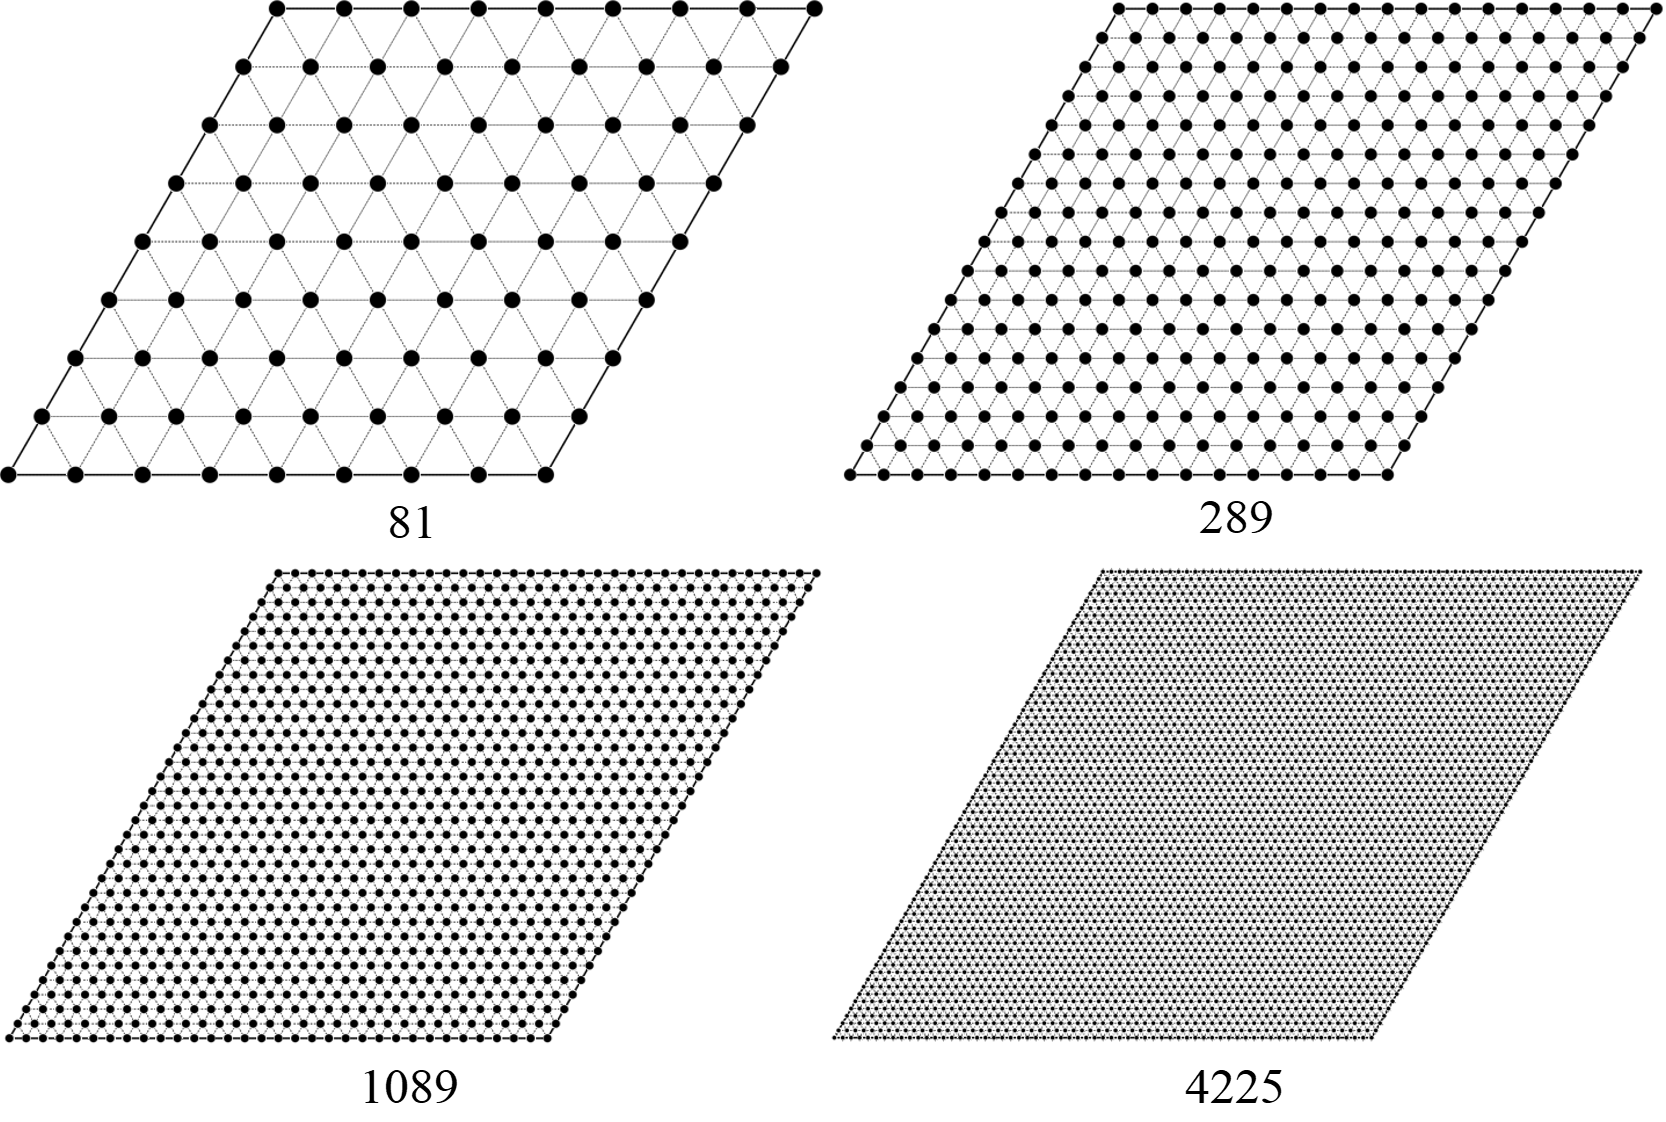
\includegraphics[scale=0.5]{figures/shearlocking/xieplatemsh.png}
        \caption{Razzaque斜板问题模型}\label{ch_5:fig:xieplatemsh}
\end{figure}
\begin{figure}[!h]
    \centering 
        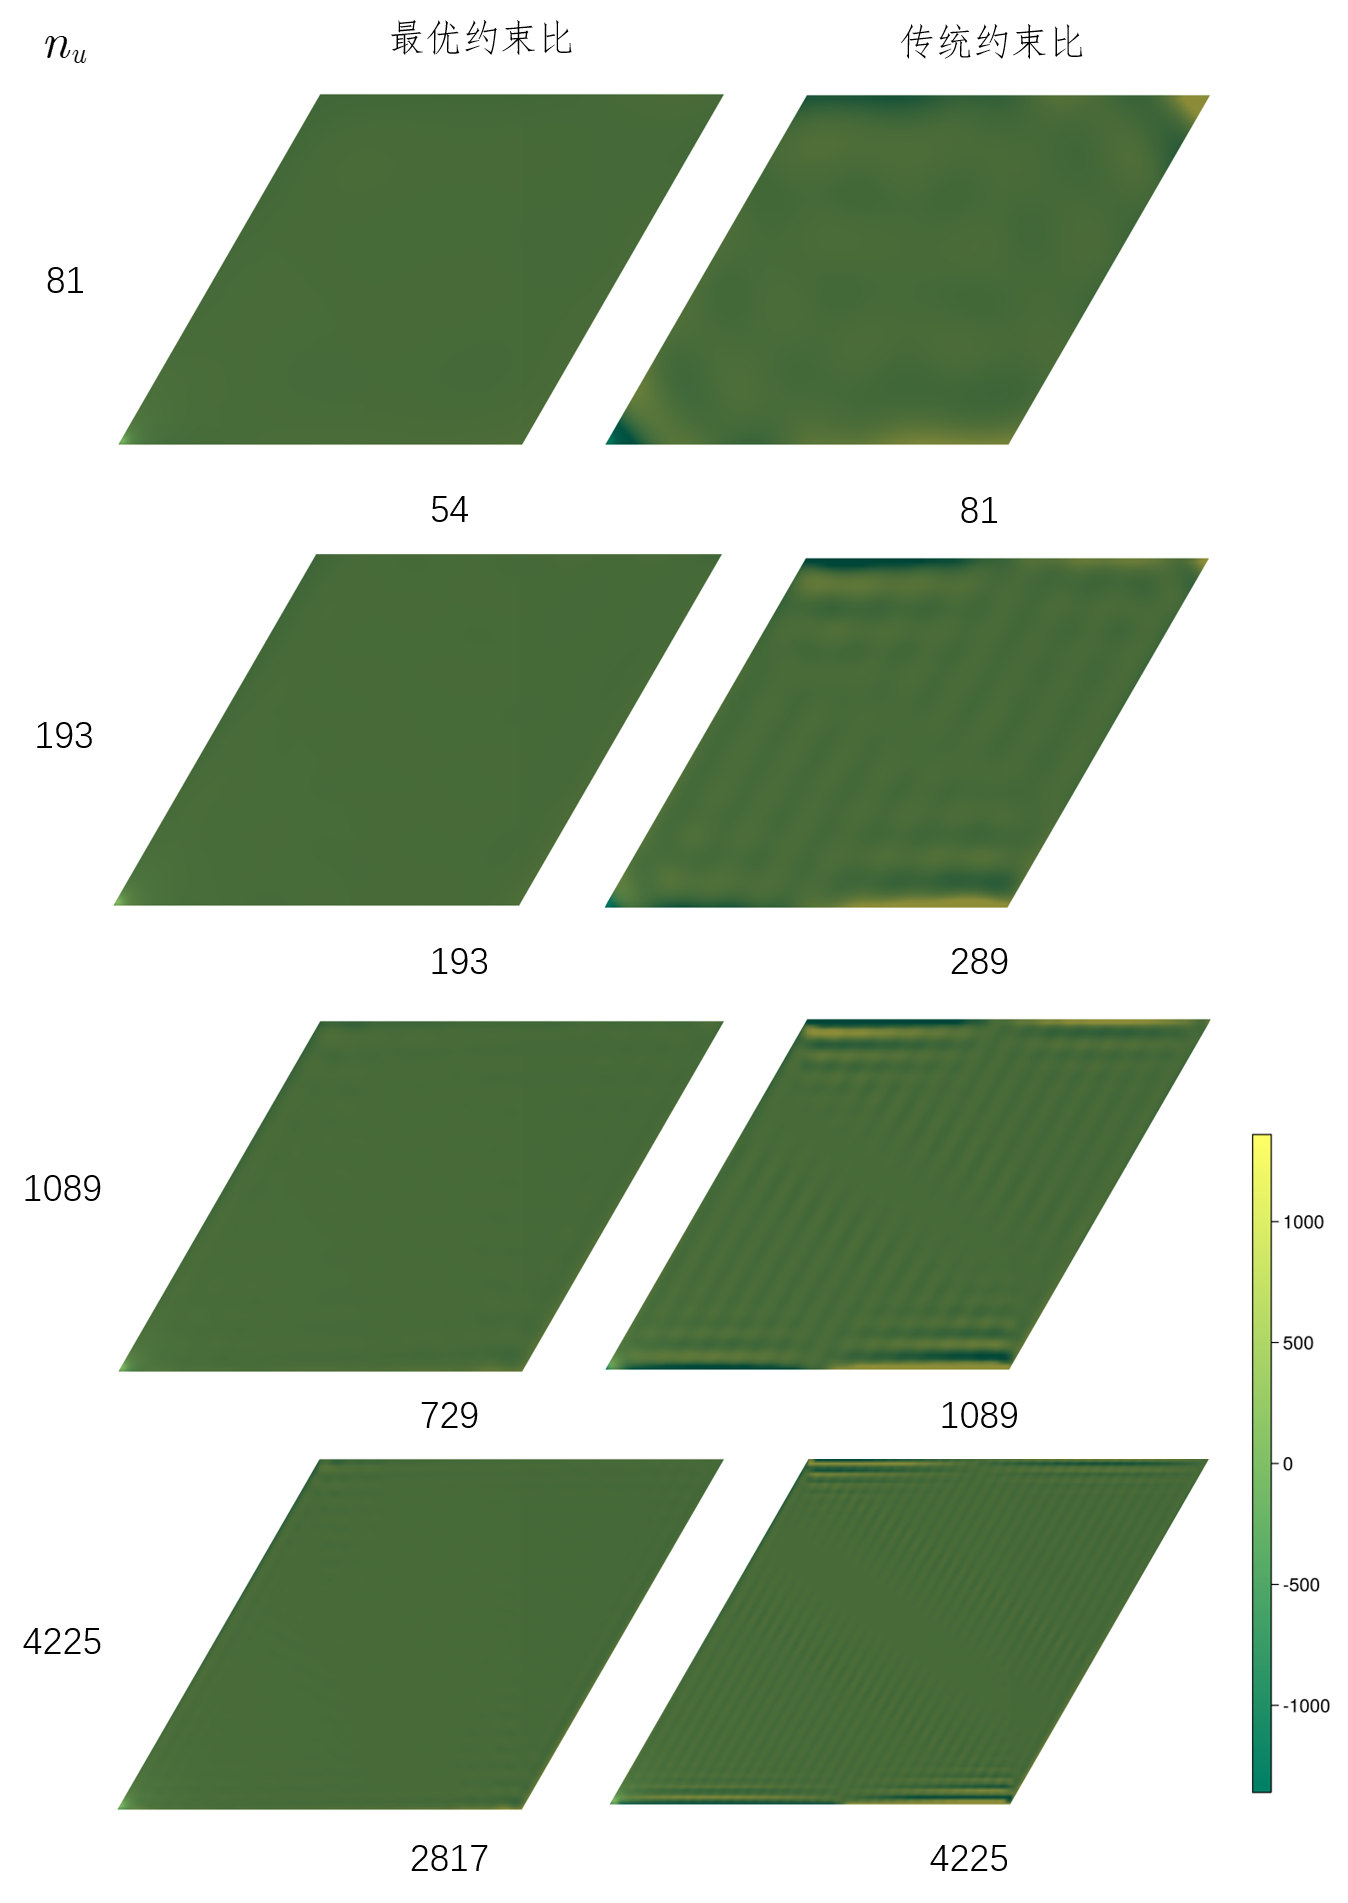
\includegraphics[scale=0.6]{figures/shearlocking/skewplateQ1_quad4.png}
        \caption{Razzaque斜板问题quad4单元应力云图($Q_1$)}\label{ch_5:fig:skewplateQ1_quad4}
\end{figure}

\begin{figure}[!h]
    \centering 
        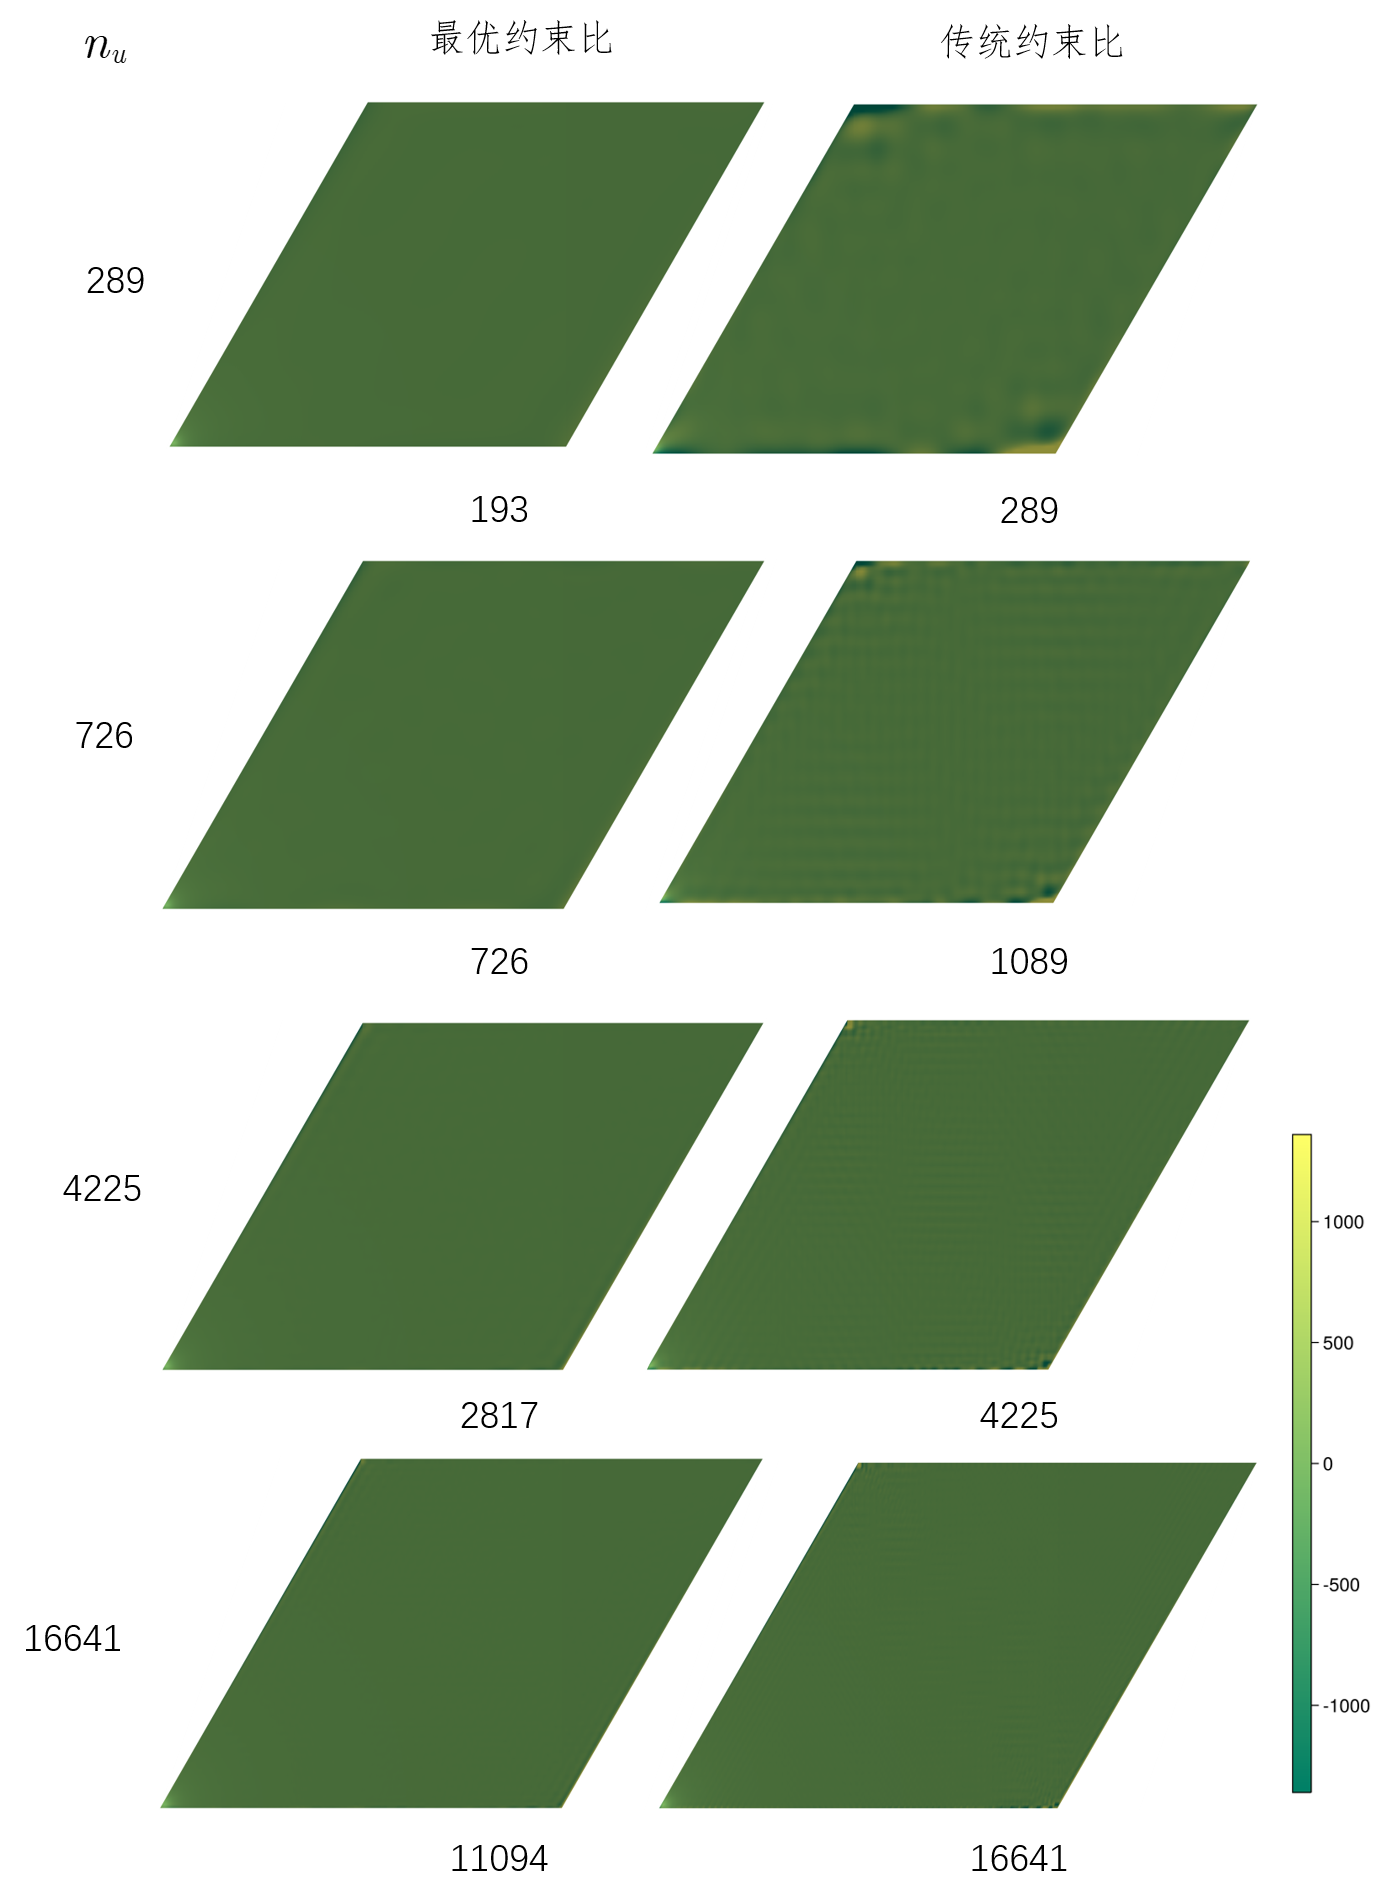
\includegraphics[scale=0.6]{figures/shearlocking/skewplateQ1_tri6.png}
        \caption{Razzaque斜板问题Tri6单元应力云图($Q_1$)}\label{ch_5:fig:skewplateQ1_tri6}
\end{figure}
\begin{figure}[!h]
    \centering 
        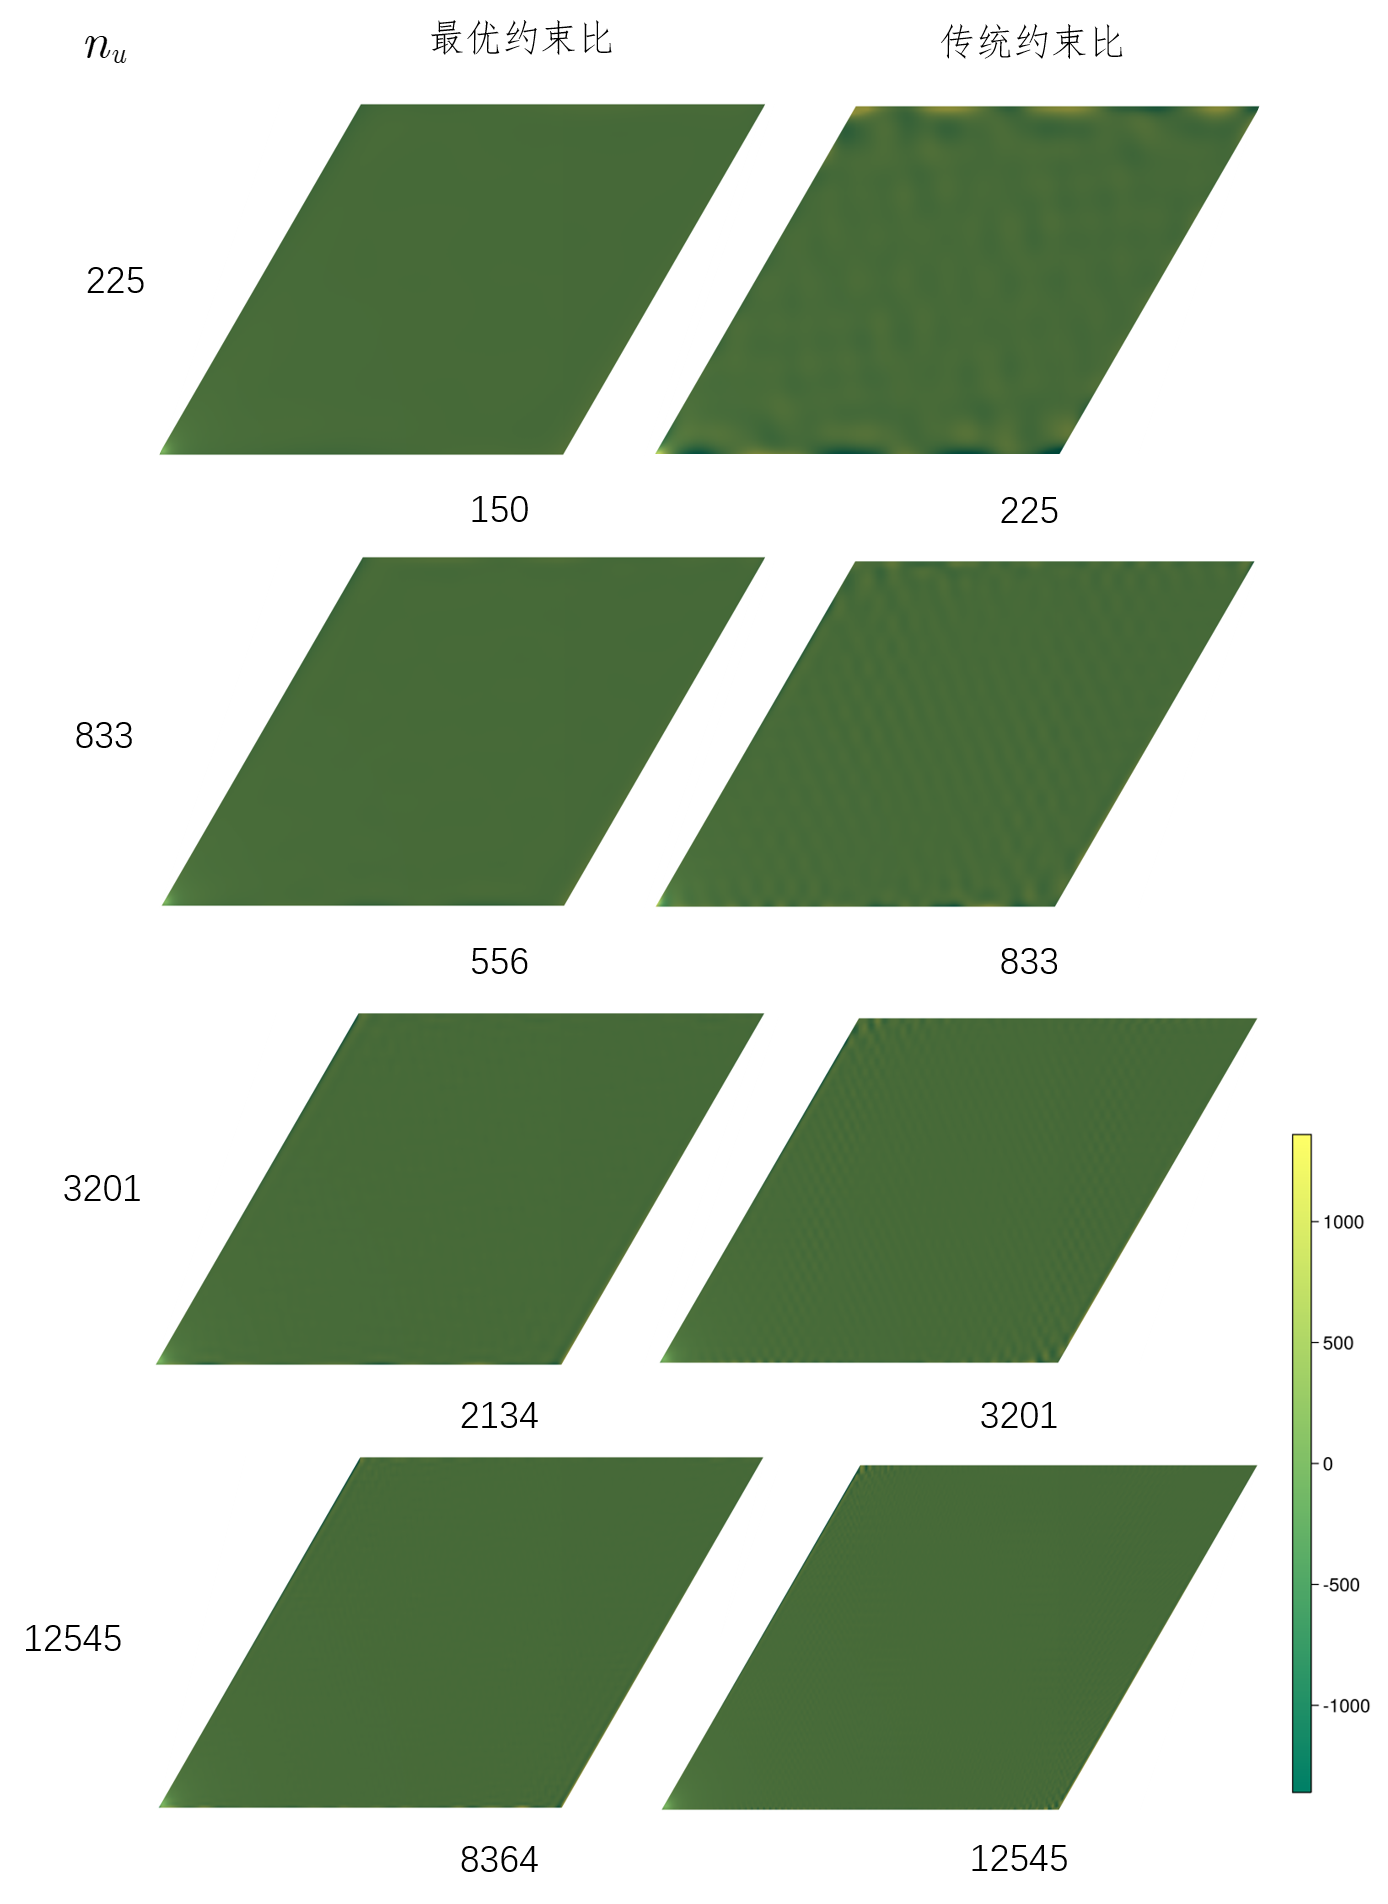
\includegraphics[scale=0.6]{figures/shearlocking/skewplateQ1_quad8.png}
        \caption{Razzaque斜板问题Quad8单元应力云图($Q_1$)}\label{ch_5:fig:skewplateQ1_quad8}
\end{figure}

\subsection{简支圆板问题}
考虑如图\ref{ch_5:fig:yuanplate}所示简支圆板问题,其中圆板的半径为$R=5$,厚度为$h$,均匀荷载作用在板内为$\bar{q}=1$,材料系数分别为杨氏模量$E=10.92$、泊松比$\nu=0.3$。该圆板中心A点位移$w_A$的精确解与板厚具有以下关系:

\begin{table} [!h]
    \centering
    \renewcommand\arraystretch{1.2}
    \caption{均匀荷载下简支圆板中心位移$w_A$}
    \begin{tabular}{cccc}
        \hline
        $h$&0.1   &1      & 2.5   \\
        $w_A$&39831 &41.599 & 3.262 \\
        \hline
    \end{tabular}
\end{table}
如图\ref{ch_5:fig:yuanplatemsh}所示,圆板求解域采用均布离散的61、217、817、3169四个疏密不同的节点进行离散,同样采用线性单元和二次单元进行数值分析。
\begin{figure}[!h]
    \centering 
        \includegraphics[scale=0.8]{figures/shearlocking/yuan plate.png}
        \caption{简支圆板问题模型}\label{ch_5:fig:yuanplate}
\end{figure}
\begin{figure}[!h]
    \centering 
        \includegraphics[scale=0.5]{figures/shearlocking/yuanplatemsh.png}
        \caption{简支圆板问题节点离散}\label{ch_5:fig:yuanplatemsh}
\end{figure}
\begin{figure}[!h]
    \centering
    \begin{tabular}{cccc}
    $\quad$&最优约束比&传统约束比\\
    $61$&\begin{subcaptiongroup}\raisebox{-0.4\height}{\includegraphics[width=0.4\textwidth]{figures/shearlocking/Circular_tri3_q1_8_6.png}}\end{subcaptiongroup}
    &\begin{subcaptiongroup}\raisebox{-0.4\height}{\includegraphics[width=0.4\textwidth]{figures/shearlocking/Circular_tri3_q1_8_8.png}}\end{subcaptiongroup}\\ 
    $217$&\begin{subcaptiongroup}\raisebox{-0.4\height}{\includegraphics[width=0.4\textwidth]{figures/shearlocking/Circular_tri3_q1_16_12.png}}\end{subcaptiongroup}
    &\begin{subcaptiongroup}\raisebox{-0.4\height}{\includegraphics[width=0.4\textwidth]{figures/shearlocking/Circular_tri3_q1_16_16.png}}\end{subcaptiongroup}\\ 
    $817$&\begin{subcaptiongroup}\raisebox{-0.4\height}{\includegraphics[width=0.4\textwidth]{figures/shearlocking/Circular_tri3_q1_32_26.png}}\end{subcaptiongroup}
    &\begin{subcaptiongroup}\raisebox{-0.4\height}{\includegraphics[width=0.4\textwidth]{figures/shearlocking/Circular_tri3_q1_32_32.png}}\end{subcaptiongroup}\\ 
    \end{tabular}
    \caption{\textbf{简支圆板问题Tri3单元应力云图($Q_1$)}}\label{ch_5:fig:YQ1_Tri3}
\end{figure}
\begin{figure}[!h]
    \centering
    \begin{tabular}{cccc}
    $\quad$&最优约束比&传统约束比\\
    $61$&\begin{subcaptiongroup}\raisebox{-0.4\height}{\includegraphics[width=0.4\textwidth]{figures/shearlocking/Circular_quad4_q1_8_6.png}}\end{subcaptiongroup}
    &\begin{subcaptiongroup}\raisebox{-0.4\height}{\includegraphics[width=0.4\textwidth]{figures/shearlocking/Circular_quad4_q1_8_8.png}}\end{subcaptiongroup}\\ 
    $217$&\begin{subcaptiongroup}\raisebox{-0.4\height}{\includegraphics[width=0.4\textwidth]{figures/shearlocking/Circular_quad4_q1_16_12.png}}\end{subcaptiongroup}
    &\begin{subcaptiongroup}\raisebox{-0.4\height}{\includegraphics[width=0.4\textwidth]{figures/shearlocking/Circular_quad4_q1_16_16.png}}\end{subcaptiongroup}\\ 
    $817$&\begin{subcaptiongroup}\raisebox{-0.4\height}{\includegraphics[width=0.4\textwidth]{figures/shearlocking/Circular_quad4_q1_32_26.png}}\end{subcaptiongroup}
    &\begin{subcaptiongroup}\raisebox{-0.4\height}{\includegraphics[width=0.4\textwidth]{figures/shearlocking/Circular_quad4_q1_32_32.png}}\end{subcaptiongroup}\\ 
    \end{tabular}
    \caption{\textbf{简支圆板问题Quad4单元应力云图($Q_1$)}}\label{ch_5:fig:YQ1_Quad4}
\end{figure}
\begin{figure}[!h]
    \centering
    \begin{tabular}{cccc}
    $\quad$&最优约束比&传统约束比\\
    $61$&\begin{subcaptiongroup}\raisebox{-0.4\height}{\includegraphics[width=0.4\textwidth]{figures/shearlocking/Circular_tri6_q1_8_6.png}}\end{subcaptiongroup}
    &\begin{subcaptiongroup}\raisebox{-0.4\height}{\includegraphics[width=0.4\textwidth]{figures/shearlocking/Circular_tri6_q1_8_8.png}}\end{subcaptiongroup}\\ 
    $217$&\begin{subcaptiongroup}\raisebox{-0.4\height}{\includegraphics[width=0.4\textwidth]{figures/shearlocking/Circular_tri6_q1_16_12.png}}\end{subcaptiongroup}
    &\begin{subcaptiongroup}\raisebox{-0.4\height}{\includegraphics[width=0.4\textwidth]{figures/shearlocking/Circular_tri6_q1_16_16.png}}\end{subcaptiongroup}\\ 
    $817$&\begin{subcaptiongroup}\raisebox{-0.4\height}{\includegraphics[width=0.4\textwidth]{figures/shearlocking/Circular_tri6_q1_32_26.png}}\end{subcaptiongroup}
    &\begin{subcaptiongroup}\raisebox{-0.4\height}{\includegraphics[width=0.4\textwidth]{figures/shearlocking/Circular_tri6_q1_32_32.png}}\end{subcaptiongroup}\\ 
    \end{tabular}
    \caption{\textbf{简支圆板问题Tri6单元应力云图($Q_1$)}}\label{ch_5:fig:YQ1_Tri6}
\end{figure}
\begin{figure}[!h]
    \centering
    \begin{tabular}{cccc}
    $\quad$&最优约束比&传统约束比\\
    $61$&\begin{subcaptiongroup}\raisebox{-0.4\height}{\includegraphics[width=0.4\textwidth]{figures/shearlocking/Circular_quad8_q1_8_6.png}}\end{subcaptiongroup}
    &\begin{subcaptiongroup}\raisebox{-0.4\height}{\includegraphics[width=0.4\textwidth]{figures/shearlocking/Circular_quad8_q1_8_8.png}}\end{subcaptiongroup}\\ 
    $217$&\begin{subcaptiongroup}\raisebox{-0.4\height}{\includegraphics[width=0.4\textwidth]{figures/shearlocking/Circular_quad4_q1_16_12.png}}\end{subcaptiongroup}
    &\begin{subcaptiongroup}\raisebox{-0.4\height}{\includegraphics[width=0.4\textwidth]{figures/shearlocking/Circular_quad8_q1_16_16.png}}\end{subcaptiongroup}\\ 
    $817$&\begin{subcaptiongroup}\raisebox{-0.4\height}{\includegraphics[width=0.4\textwidth]{figures/shearlocking/Circular_quad4_q1_32_26.png}}\end{subcaptiongroup}
    &\begin{subcaptiongroup}\raisebox{-0.4\height}{\includegraphics[width=0.4\textwidth]{figures/shearlocking/Circular_quad8_q1_32_32.png}}\end{subcaptiongroup}\\ 
    \end{tabular}
    \caption{\textbf{简支圆板问题Quad8单元应力云图($Q_1$)}}\label{ch_5:fig:YQ1_Quad8}
\end{figure}

\section{小结}
